% !TeX encoding = UTF-8
% !TeX TS-program = xelatex
% !TeX spellcheck = en_GB
\documentclass[12pt,a4paper]{scrbook}

% Input Type and AMS-Packages
\usepackage{amsmath,amsfonts,amssymb,amsthm}
\usepackage{unicode-math}

% Typography
\usepackage{fontspec}
\setmainfont[Ligatures=TeX]{EB Garamond}
\newfontfamily\headingfont[RawFeature={+c2sc,+scmp},
                           Ligatures=TeX,
                           Letters=SmallCaps]{EB Garamond}
\setsansfont[Ligatures=TeX, Scale=MatchLowercase]{Open Sans}
\setmonofont[Scale=MatchLowercase]{Fira Mono}
\newfontfamily\monomath[Scale=MatchUppercase]{Fira Mono}
\setmathfont[Scale=MatchUppercase]{STIX Two Math}
\setmathrm[Scale=MatchUppercase,
           BoldFont=STIX Two Text Bold]{STIX Two Math}
\setmathtt[Scale=MatchUppercase]{Fira Mono}


\renewcommand{\scshape}{\headingfont}

\usepackage{polyglossia}
\setdefaultlanguage[variant=british]{english}
\setotherlanguage{german}
\usepackage{floatrow}
\usepackage{booktabs}

\usepackage[autostyle,
            english=british]{csquotes}
\usepackage{microtype}
\usepackage{enumitem}
\usepackage{subcaption}

\usepackage{letltxmacro}

\newlist{thmlist}{enumerate}{1}			% thmlist-s may only be used in theorem environments
\setlist[thmlist]{label=(\roman{thmlisti}),
                  ref=\thethm.(\roman{thmlisti}),
                  noitemsep}
\newlist{exlist}{enumerate}{1}
\setlist[exlist]{label=(\arabic{exlisti}),
                 ref=\thethm.(\arabic{exlisti}),
                 noitemsep,
                 wide=\parindent,
                 listparindent=\parindent}
\newlist{plist}{enumerate}{1}
\setlist[plist]{label=(\roman{plisti}),
                ref=(\roman{plisti}),
                noitemsep,
                wide=\parindent,
                listparindent=\parindent}
\newlist{clist}{enumerate}{2}
\setlist[clist]{label*=(\alph*),
                ref=(\alph*),
                noitemsep,
                wide=\parindent,
                listparindent=\parindent}

\usepackage{setspace}
\renewcommand{\arraystretch}{1.5}


\usepackage{listingsutf8}	% Typeset code.
\lstset{extendedchars=true,
        basicstyle=\ttfamily\small,
        commentstyle=\color{gray},
        stringstyle=\color{darkgray},
        xleftmargin=\parindent,
        showstringspaces=false,
        language=haskell}

% BibLaTex
\usepackage[style=numeric,backend=biber]{biblatex}
\addbibresource{./references.bib}


% Math, Operators and Theorems
\usepackage{thmtools}	% More Flexibility in Theorem Styles + Provides in Combination with ref-Packages the
						% Possibility to Refer to Theorem Style in Reference.

\numberwithin{equation}{section}

\DeclareMathOperator{\N}{\mathbb{N}}
\DeclareMathOperator{\Z}{\mathbb{Z}}
\DeclareMathOperator{\Q}{\mathbb{Q}}
\DeclareMathOperator{\R}{\mathbb{R}}
\DeclareMathOperator{\C}{\mathbb{C}}
\DeclareMathOperator{\F}{\mathbb{F}}

\DeclareMathOperator{\Aut}{Aut}
\DeclareMathOperator{\id}{id}

\DeclareMathOperator{\kernel}{ker}
\DeclareMathOperator{\im}{im}
\DeclareMathOperator{\rk}{rk}
\DeclareMathOperator{\End}{End}
\DeclareMathOperator{\Hom}{Hom}
\DeclareMathOperator{\Mod}{mod}
\DeclareMathOperator{\D}{D}
\DeclareMathOperator{\lcm}{\mathrm{lcm}}
\DeclareMathOperator{\ord}{\mathrm{ord}}
\DeclareMathOperator{\Quot}{Quot}

\newcommand*{\sta}{\text{\monomath §}}
\newcommand*{\emp}{\text{\monomath \_}}
\newcommand*{\zer}{\mathtt{0}}
\newcommand*{\one}{\mathtt{1}}
\newcommand*{\state}[1]{s_{\text{#1}}}
\newcommand*{\sstart}{\state{start}}
\newcommand*{\shalt}{\state{halt}}
\newcommand*{\scheck}{s_{\text{check}}}
\newcommand*{\enc}[1]{\ulcorner #1 \urcorner}
\newcommand*{\rel}[1]{\mathrel{\MakeUppercase #1}}
\newcommand*{\algint}[1][K]{\mathcal{O}_{#1}}
\newcommand*{\modalgint}[1][K]{\mathfrak{O}_{#1}}
\newcommand*{\Norm}[1][L/K]{\mathrm N_{#1}}
\newcommand*{\px}{\mathrm x}
\newcommand*{\py}{\mathrm y}
\newcommand*{\sigmaK}[1]{{\left(#1\right)}^*}
\newcommand*{\lang}{\mathcal{L}}
\newcommand*{\seq}[2][n]{#2_{1},\ldots,#2_{#1}}
\newcommand{\set}[1]{\left\lbrace #1 \right\rbrace}

\usepackage{newunicodechar}
\newunicodechar{√}{\sqrt}
\makeatletter
\newcommand{\dotminus}{\mathbin{\text{\@dotminus}}}

\newcommand{\@dotminus}{%
  \ooalign{\hidewidth\raise1ex\hbox{.}\hidewidth\cr$\m@th-$\cr}%
}
\makeatother

\NewNegationCommand{∈}{\notin}


\declaretheoremstyle[
    spaceabove=6pt, spacebelow=6pt,
    headfont=\headingfont,
    notefont=\mdseries, notebraces={(}{)},
    bodyfont=\itshape,
    postheadspace=0.5\parindent
    ]{mythm}
\declaretheoremstyle[
    spaceabove=6pt, spacebelow=6pt,
    headfont=\headingfont,
    notefont=\mdseries, notebraces={(}{)},
    bodyfont=\normalfont,
    postheadspace=0.5\parindent
    ]{mydef}

\declaretheorem[
	name=Theorem,
    style=mythm,
  	refname={theorem,theorems},		%Lower Case Versions of Theorem Type
  	Refname={Theorem,Theorems},
  	numberwithin=section]{thm}
\declaretheorem[
	name=Lemma,
    style=mythm,
	refname={lemma,lemmas},
	Refname={Lemma,Lemmas},
	sibling=thm]{lem}
\declaretheorem[
	name=Proposition,
    style=mythm,
	refname={proposition,propositions},
	Refname={Proposition,Propositions},
	sibling=thm]{pro}
\declaretheorem[
	name=Corollary,
    style=mythm,
	refname={corollary,corollarys},
	Refname={Corollary,Corollarys},
	sibling=thm]{cor}

\declaretheorem[
	name=Definition,
	style=mydef,
	numbered=no]{defin}
\declaretheorem[
	name=Example,
	style=mydef,
	sibling=thm]{exam}

\declaretheorem[
  name=Problem,
  style=mydef,
  numbered=no]{problem}
\declaretheorem[
  name=Church-Turing thesis,
  style=mydef,
  numbered=no]{churchturing}

\declaretheorem[
	name=Remark,
	style=remark,
	numbered=no]{rem}


%TikZ and TikZ-Styles
\usepackage{tikz}

% References
\usepackage{hyperref}
\usepackage[capitalize]{cleveref}

\hypersetup{
	pdftitle={On Hilbert's Tenth Problem over Rings of Algebraic Integers},
	pdfauthor={Tim Benedikt Herbstrith},
  pdflang={en-GB},
  pdfkeywords={Number Theory, Theoretical Informatics, Hilbert's 10th Problem}}

\Crefname{thm}{Thm}{Thms}
\Crefname{lem}{Lem.}{Lem.}
\Crefname{pro}{Prop.}{Props}
\Crefname{cor}{Cor.}{Cors}
\Crefname{exam}{Example}{Examples}

\addtotheorempostheadhook[thm]{\crefalias{thmlisti}{thm}}
\addtotheorempostheadhook[lem]{\crefalias{thmlisti}{lem}}
\addtotheorempostheadhook[pro]{\crefalias{thmlisti}{pro}}
\addtotheorempostheadhook[cor]{\crefalias{thmlisti}{cor}}
\addtotheorempostheadhook[exam]{\crefalias{exlisti}{exam}}

% ------------------------------------------------------------------------------
% Only for drafts!
\usepackage{todonotes}
\usepackage{showlabels}	%Used in Drafts to Print references.
%-------------------------------------------------------------------------------
%-------------------------------------------------------------------------------


\begin{document}

% ######## ########   #######  ##    ## ######## 
% ##       ##     ## ##     ## ###   ##    ##
% ##       ##     ## ##     ## ####  ##    ##
% ######   ########  ##     ## ## ## ##    ##
% ##       ##   ##   ##     ## ##  ####    ##
% ##       ##    ##  ##     ## ##   ###    ##
% ##       ##     ##  #######  ##    ##    ##


% Using Layers in TikZ
\pgfdeclarelayer{background}
\pgfsetlayers{background,main}

% Page Breaks for Displayed Formulas
\allowdisplaybreaks

\frontmatter

% !TEX encoding = UTF-8
% !TEX TS-program = xelatex
% !TEX spellcheck = en_GB
% !TEX engine = xelatex
% !TEX root = ../Herbstrith-H10_over_AI.tex

% ######## ########   #######  ##    ## ########
% ##       ##     ## ##     ## ###   ##    ##
% ##       ##     ## ##     ## ####  ##    ##
% ######   ########  ##     ## ## ## ##    ##
% ##       ##   ##   ##     ## ##  ####    ##
% ##       ##    ##  ##     ## ##   ###    ##
% ##       ##     ##  #######  ##    ##    ##

\begin{titlepage}
%\vspace*{-2cm}  % bei Verwendung von vmargin.sty
\begin{flushright}
    
\includegraphics{uni-logo}
\end{flushright}
\vspace{0.5cm}

\begin{center}  % Diplomarbeit ODER Magisterarbeit ODER Dissertation
    \Huge{\textsf{\textbf{\MakeUppercase{
        Masterarbeit
    }}}}
    \vspace{1.5cm}

    \large{\textsf{  % Diplomarbeit ODER Magisterarbeit ODER Dissertation
                     % (Dies ist erst die Ueberschrift!)
        Titel der Masterarbeit
    }}
    \vspace{.1cm}

    \LARGE{\textsf{ On Hilbert's Tenth Problem over\\
                    Rings of Algebraic Integers
    }}
    \vfill

    \large{\textsf{  % Verfasserin ODER Verfasser (Ueberschrift)
        Verfasser
    }}

    \Large{\textsf{  Tim Benedikt Herbstrith
    }}
    \vfill

    \large{\textsf{
        angestrebter akademischer Grad  % (Ueberschrift)
    }}

    \Large{\textsf{  % Magistra ODER Magister ODER Doktorin ODER Doktor
                     % ACHTUNG: Kuerzel "Mag.a" oder "Dr.in" nicht zulaessig
        Master of Science (MSc.)
    }}

\vspace{1.5cm}

\noindent\textsf{Wien, im Monat September 2018}
  % <<<<< ORT, MONAT UND JAHR EINTRAGEN
\vfill

\noindent\begin{tabular}{@{}ll}
\textsf{Studienkennzahl lt.\ Studienblatt:}
&
\textsf{A 033 821}  % <<<<< STUDIENKENNZAHL EINTRAGEN
\\
    % BEI DISSERTATIONEN:
%\textsf{Dissertationsgebiet lt. Studienblatt:}
    % ANSONSTEN:
\textsf{Studienrichtung lt.\ Studienblatt:}
&
\textsf{Mathematik}  % <<<<< DISSGEBIET/STUDIENRICHTUNG EINTRAGEN
\\
% Betreuerin ODER Betreuer:
\textsf{Betreuer: }
&
\textsf{ao.~Univ.-Prof.~Mag.~Dr.~Ch.~Baxa}  % <<<<< NAME EINTRAGEN
\end{tabular}
\end{center}
\end{titlepage}

\newpage%
\thispagestyle{empty}%
\vspace*{\fill}%
\noindent%
\begin{footnotesize}%
If not stated otherwise, \emph{On Hilbert's Tenth Problem over Rings
of Algebraic Integers} by Tim B. Herbstrith is licenced under a \textsc{Creative
Commons Attribution-NonCommercial-ShareAlike 4.0 International License}. All
code snippets are provided `as is' without warranty of any kind, express or
implied, including but not limited to the warranties of merchantability, fitness
for a particular purpose and non-infringement under the terms of the
\textsc{MIT} licence. The source codes and the aforementioned licences are
published at
\begin{center}
 \url{https://github.com/tim6her/h10-over-rings-of-integers}
\end{center}
\end{footnotesize}
\cleardoublepage


\begin{german}
\section*{Vorwort}
\todo{Schreibe das Vorwort}
\end{german}

\vspace{1.5cm}

\section*{Abstract}
\todo{Write the abstract}
\newpage
\thispagestyle{empty}
\tableofcontents


\mainmatter

% ##     ##    ###    #### ##    ##
% ###   ###   ## ##    ##  ###   ##
% #### ####  ##   ##   ##  ####  ##
% ## ### ## ##     ##  ##  ## ## ##
% ##     ## #########  ##  ##  ####
% ##     ## ##     ##  ##  ##   ###
% ##     ## ##     ## #### ##    ##

\chapter{Prerequisites and central notions}

To tackle Hilbert's tenth problem over some rings of algebraic integers we need
to define three central notions. Firstly, we should formalize what we mean by a
‘process [with] a finite number of operations’~\cite{Hilbert1900}; secondly, it
must be defined what it means to determine the solvability of an equation; and
thirdly, we must replace one or both occurrences of rational integers by
elements of other rings.

The first section of the preliminaries will settle our first task and give a
definition of computability. The second section will provide the techniques
required to view polynomials with roots as natural numbers and helps us derive
natural variants of Hilbert's tenth problem. The third section of the
preliminaries is devoted to defining algebraic integers and will remind the
reader of some of their important properties.

Throughout this thesis the symbol \(ℕ\) shall denote the set of non-negative
integers \(\set{0, 1, 2, …}\).

\section{Prerequisites from computability theory}
% !TeX encoding = UTF-8
% !TeX TS-program = xelatex
% !TeX engine=xelatex
% !TeX spellcheck = en_GB
% !TeX root = ../Herbstrith-H10_over_AI.tex

In this section I closely follow the lecture notes on the subject by
\textcite{Mueller2016}.

\begin{defin}
  A \emph{(decision) problem} is a subset of the set of finite
  $\zer$-$\one$-strings $\lbrace \zer, \one \rbrace^*$ including the
  empty string $λ$. One calls $\lbrace \zer, \one \rbrace$
  \emph{alphabet} and its elements \emph{bits.}
\end{defin}

One immediate objection against this definition is that not all problems
arise as subsets of these strings. However, such problems $Q$ are
captured up to an encoding.

\[ \enc{\cdot} : Q → \lbrace \zer, \one \rbrace^*\]

One usually does not concern oneself with the details of this encoding.
However, the encoding should capture the structure of the problem---a notion
that will be made precise in \cref{sec:computable structures}.

\begin{exam}
  Consider the problem of deciding whether a finite simple graph is
  connected or not. If one demands the vertex set to be of the form
  $\set{0, 1, …, n}$, then the set of all graphs can be encoded
  as the set of the respective adjacency matrices written as a string
  \[
    b_{00}b_{01} …b_{0n}b_{10}…b_{nn}
  \]
  of length $(n + 1)^2$, where $b_{ij} = \one$ if and only if the
  vertices $i$ and $j$ are connected.
\end{exam}

\begin{defin}
  A \emph{Turing machine} $\mathbb A$ on the \emph{alphabet}
  $A = \lbrace \sta, \emp, \zer, \one \rbrace$ is a tuple $(S, δ)$,
  where $\sstart, \shalt ∈ S$ is a finite non-empty set, called
  \emph{set of states}, and
  \[
    δ: S × A → S × A × \lbrace -1, 0, 1 \rbrace
  \]
  is called \emph{transition function}. If $δ(s, a) = (s', b, m)$, one
  demands that the following axioms are satisfied

  \begin{thmlist}
  \item
    $a = \sta$ if and only if $b = \sta$,
  \item
    If $a = \sta$, then $m ≠ -1$, and
  \item
    If $s = \shalt$, then $s' = \shalt$, $a = b$ and $m = 0$.
  \end{thmlist}
\end{defin}

Informally, one can think of a Turing machine as a device, consisting of a
\emph{work-tape} and a \emph{head}. The work-tape stores all the information in
cells arranged in a consecutive order. Each of these cells contains a letter
from the alphabet.

Let us look at the example of the Turing machine in \cref{fig:Turing machine}.
During the run of the machine the head reads the symbol $\zer$ at the current
position and the machine evaluates the transition function $δ$ at $\zer$ and the
current state $\state{overflow}$. Now assume that
\[
  δ(\state{overflow}, \zer) = (\state{return}, \one, -1).
\]
One interprets this in the following way. The Turing machine changes its state
to $\state{return}$, the head writes $\one$ in the current cell and moves one
cell to the left. The movement is determined by the last item of the triple
$δ(\state{overflow}, \zer)$, where $-1$ indicates moving to the left, $1$
indicates moving to the right, and $0$ indicates not moving at all.

\begin{figure}
  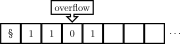
\includegraphics{res/turing_add1_4}
  \caption{A Turing machine}
  \label{fig:Turing machine}
\end{figure}

\begin{defin}
  Let $\mathbb A = (S, δ)$ be a Turing machine. A \emph{configuration}
  of $\mathbb A$ is a triple $(s, j, c) ∈ S × ℕ × A^ℕ$. It reflects
  the current state of $\mathbb A$, the current position of its
  head, and the content of its work-tape.
\end{defin}

A configuration of the form $(\shalt, 0, c)$ is called \emph{halting}. A
\emph{start configuration} is of the form $(\sstart, 0, c)$ such that $c(0) =
\sta$ and there exists an $n ∈ ℕ$ such that $c(i) = \emp$ if and only if $i >
n$. This means that in a start configuration the work-tape reads
\[
  \sta x_1 x_2 … x_n \emp \emp …
\]
It will be very convenient to identify the finite string $x_1…x_n$ with this
tape content.

\begin{defin}
  One writes $(s, j, c) \vdash_1 (s', j', c')$ and calls $(s', j', c')$ a
  \emph{successor configuration} of $(s, j, c)$ if there exists an $m ∈ \lbrace
  -1, 0, 1 \rbrace$ such that

  \begin{itemize}
  \item
    $δ(s, c) = (s', c', m)$,
  \item
    $j' = j + m$, and
  \item
    $c'(ℓ) = c(ℓ)$ for all $ℓ ≠ j$.
  \end{itemize}

  This relation makes the set of all configurations of $\mathbb A$ into a
  directed graph. A \emph{run} of $\mathbb A$ on $x$ is a path in this directed
  graph starting at the start configuration $(\sstart, 0, x)$. A run of
  $\mathbb A$ on $x$ is \emph{halting} or \emph{complete} if it reaches a
  halting configuration $(\shalt, 0, y)$. In this case I write $\mathbb A (x) =
  y$.
\end{defin}

I will denote Turing machines using listings, where the fact that
$δ_\text{delta} (\state{state}, b) = (\state{state'}, c, m)$ is encoded by

\begin{lstlisting}
delta "state" c = ("state'", c', m)
\end{lstlisting}

Variables \verb+c+ match all possible states or characters in the alphabet
respectively. However, I follow the convention that if an assignment of
variables matches more than one pattern, the first matching pattern is chosen.
This means that
%
\begin{lstlisting}
delta "state" 1 = ("state'", 1, 1)
delta "state" c = ("state''", c, 0)
\end{lstlisting}
%
should be interpreted as
%
\[ δ(s, c) =
  \begin{cases}
    (\state{state'}, \one, 1) & \text{if } s=\state{state} ∧ c = \one\\
    (\state{state''}, c, 0) & \text{if } s=\state{state} ∧ c ≠ \one
  \end{cases}.
\]

See \cref{app:turing} on how to simulate Turing machines
using the \emph{Haskell} programming language.

\begin{exam}
    Consider the Turing machine $\mathbb A_\text{add1} = (\lbrace \sstart,
    \shalt, \state{overflow}, \state{return}, \state{error} \rbrace,
    δ_\text{add1})$ that adds $1$ to a (possibly zero-patched) binary
    representation of a natural number $n$. Its transition function is described
    in \cref{lst:add1}. The last line of the program ensures, that $δ$ is a
    total function, as it matches all remaining pairs of states and
    characters and lets the machine enter the state $\state{error}$. The
    complete run of $\mathbb A_\text{add1}$ on $\one\one\zer\one$ can be seen in
    \cref{fig:complete run}.
\end{exam}

\lstinputlisting[float, frame=tb,
                 caption=A Turing machine adding one to the input string,
                 label=lst:add1]{./listings/add1.hs}

\begin{figure*}
    \begin{subfigure}{.5\textwidth}
        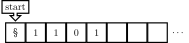
\includegraphics{res/turing_add1_1}
        \caption{$δ(\sstart, \sta) = (s_\text{overflow}, \sta, 1)$}
    \end{subfigure}

    \begin{subfigure}{.5\textwidth}
        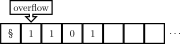
\includegraphics{res/turing_add1_2}
        \caption{$δ(s_\text{overflow}, \one) = (s_\text{overflow}, \one, 1)$}
    \end{subfigure}

    \begin{subfigure}{.5\textwidth}
        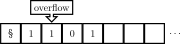
\includegraphics{res/turing_add1_3}
        \caption{$δ(s_\text{overflow}, \one) = (s_\text{overflow}, \one, 1)$}
    \end{subfigure}

    \begin{subfigure}{.5\textwidth}
        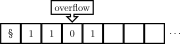
\includegraphics{res/turing_add1_4}
        \caption{$δ(s_\text{overflow}, \zer) = (s_\text{return}, \one, -1)$}
    \end{subfigure}

    \begin{subfigure}{.5\textwidth}
        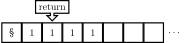
\includegraphics{res/turing_add1_5}
        \caption{$δ(s_\text{return}, \one) = (s_\text{return}, \one, -1)$}
    \end{subfigure}

    \begin{subfigure}{.5\textwidth}
        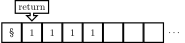
\includegraphics{res/turing_add1_6}
        \caption{$δ(s_\text{return}, \one) = (s_\text{return}, \one, -1)$}
    \end{subfigure}

    \begin{subfigure}{.5\textwidth}
        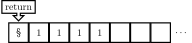
\includegraphics{res/turing_add1_7}
        \caption{$δ(s_\text{return}, \sta) = (s_\text{halt}, \sta, 0)$}
    \end{subfigure}

    \begin{subfigure}{.5\textwidth}
        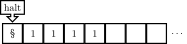
\includegraphics{res/turing_add1_8}
        \caption{$δ(s_\text{halt}, \sta) = (s_\text{halt}, \sta, 0)$}
    \end{subfigure}

    \caption{The complete run of $\mathbb A_\text{add1}$ on $\one\one\zer\one$}
    \label{fig:complete run}
\end{figure*}

\begin{defin}
    Let $\mathbb A$ be a Turing machine.

    \begin{thmlist}
        \item
          $\mathbb A$ \emph{computes} the partial function that maps each
          $x$ with a complete run to $\mathbb A(x)$ and is undefined for all
          other strings.
        \item
          $\mathbb A$ \emph{accepts} all $x$ such that
          $\mathbb A(x) = \one$ and \emph{rejects} them if
          $\mathbb A(x) = \zer$.
        \item
          A partial function on $\lbrace \zer, \one \rbrace^*$ is
          \emph{computable} if there is a Turing machine computing it. Sometimes
          computable functions are referred to as \emph{recursive} or
          \emph{efficient} functions.
        \item
          A subset of $\lbrace \zer, \one \rbrace^*$, i.e. a
          problem, is \emph{decidable} if there is a Turing machine computing
          its characteristic function.
        \item
          A problem is called \emph{semi-decidable} or \emph{computably
          enumerable} if there is a Turing machine accepting precisely the
          elements of the problem.
    \end{thmlist}
\end{defin}

The last item of the definition above means that a problem is
semi-decidable if there is a Turing machine affirming membership of the
corresponding set but it might not be able to refute membership.

Note that every finite problem is decidable by a Turing machine that reads the
tape content and checks at every step whether there are elements in the problem
that start with the tape content the machine has read. After $n + 1$ steps,
where $n$ denotes the length of the longest string in the problem, the machine
stops at the latest.

\begin{lem} \label{lem:composition of Turing machines}
  Let $\mathbb A_1 = (S_1, δ_1)$ and $\mathbb A_2 = (S_2, δ_2)$ be Turing
  machines computing $f_1: D_1 → \set{\zer, \one}^*$ and $f_2: D_2 → \set{\zer,
  \one}^*$ respectively ($D_1, D_2 \subseteq \set{\zer, \one}^*$). Then there
  exists a Turing machine $\mathbb A_{f_2 \circ f_1}$ computing the partial
  function $f_2 \circ f_1: D_1 ∩ f_1^{-1}(D_2) → \set{\zer, \one}^*$ obtained by
  composing $f_1$ and $f_2$.
\end{lem}
\begin{proof}
  One constructs $\mathbb A_{f_2 \circ f_1}$ from $\mathbb A_1$ and $\mathbb
  A_2$ as follows. Let $S_1 = \set{\sstart, \shalt} \sqcup S_1'$ and $S_2 =
  \set{\sstart, \shalt} \sqcup S_2'$, then set $S = \set{\sstart, \shalt} \sqcup
  S_1' \sqcup S_2' \sqcup \set{\state{compose}}$, where $\sqcup$ denotes the
  disjoint union. Now set for $c ∈ A$
  %
  \begin{align*}
    δ (s, c) &=
      \begin{cases}
        δ_1 (s, c) & \text{if } s ∈ S_1' ∪ \set\sstart \\
        (\state{compose}, c', m) & \text{if } s ∈ S_1 \text{ and } δ_1(s, c) = (\shalt, c', m)\\
        δ_2 (s, c) & \text{if } s ∈ S_2' ∪ \set\shalt \\
      \end{cases}, \\
    δ (\state{compose}, c) &= δ_2 (\sstart, c).
  \end{align*}
  %
  Then $\mathbb A_{f_2 \circ f_1} = (S, δ)$ computes $f_1 \circ f_2$ because $δ$
  is defined to first run the program of $\mathbb A_1$ and if this machine would
  reach a halting state run $\mathbb A_2$.
\end{proof}
% IDEA Maybe: A semi-decidable set is decidable iff its complement is semi-decidable
\todo{Maybe: A semi-decidable set is decidable iff its complement is semi-decidable}

\begin{exam}
    One can encode a natural number $n$

    \begin{exlist}
    \item \label{ex:tally encoding}
      in tally notation
      \begin{align*}
        n & ↦ \underbrace{\one…\one}_{n\text{-times}}, \quad \text{if } n > 0 \\
        0 & ↦ λ
      \end{align*}
    \item
      by its binary representation
      \begin{align*}
          n = 2^k + \sum_{i = 0}^{k-1} b_i 2^i & ↦ b_0…b_{k-1}\one, \quad
              \text{if } n > 0\\
                                             0 & ↦ \zer,
      \end{align*}
      or
    \item \label{ex:omega encoding}
      by a shifted and truncated form of its binary representation
      \begin{align*}
        n = 1 + \sum_{i = 0}^k b_i 2^i & ↦ b_0…b_k, \quad \text{if } n > 0\\
                                     0 & ↦ λ
      \end{align*}

      In other words, $n$ is mapped to the $n$-th string if one orders $\lbrace
      \zer, \one \rbrace ^ ℕ$ lexicographically. Following a tradition in
      logics I denote $ℕ$ under this last encoding by $ω$.
    \end{exlist}

    In either case the set obtained by encoding $ℕ$ is easily seen to be
    decidable. In the first case, check that the string contains only copies
    of the bit $\one$. Indeed, this can be achieved by the Turing machine
    %
    \[\mathbb A_\text{tally} =
      ( \lbrace \sstart, \shalt, \scheck, \state{accept}, \state{reject},
        \state{rejectMR}, \state{error} \rbrace, δ),\]
    %
    whose transition function is displayed in \cref{lst:tally encoding}.

    In the second case it suffices to check that the string has length $1$
    or ends in an $\one$, and in the third case every string is accepted.
\end{exam}

\lstinputlisting[float, frame=tb,
                 caption=A Turing machine checking whether the input is tally-encoded,
                 label=lst:tally encoding]{./listings/tally.hs}

Taking another look at the definition of computability, one sees that only unary
functions defined on subsets of $ω$, mapping to subsets of $ω$ can be
computable. However, one can easily extend this to functions on multiple
variables, by encoding tuples in $ω \times ω$ by elements of $ω$ in such a way,
that the projections $p_i: \enc{(x_1, x_2)} ↦ x_i$  for $i ∈ \lbrace 0, 1
\rbrace$ are uniformly computable. This means, there are injective pairing
functions $ω^2 → ω$ and Turing machines $\mathbb P_1, \mathbb P_2$
computing $p_1$ or $p_2$ respectively. Clearly if one has a pairing function $ℕ^2 → ℕ$ then one immediately obtains a pairing function $ω^2 → ω$
by composing with the encoding function.

\begin{exam}[Pairing functions]
  \begin{exlist}
    \item\label{ex:tally pairing}
    Using tally notation on can encode $(n, m) ∈ ℕ^2$ by
    \[
      ⟨\enc{n}, \enc{m}⟩ = \underbrace{\one … \one}_{n\text{-times}} \zer \underbrace{\one … \one}_{m\text{-times}}
    \]

    \item A simple pairing function encodes the pair $(b_1b_2…b_n, c_1c_2…c_m) ∈ ω^2$

    \[ ⟨b_1b_2…b_n, c_1c_2…c_m⟩ = b_1b_1b_2b_2…b_nb_n \zer\one c_1c_2…c_m. \]
  \end{exlist}
\end{exam}

Of course by applying a pairing function iteratively one obtains an $n$-ary pairing function. The projections need to be composed accordingly. For example
\[
  (x_1, x_2, x_3) ↦ ⟨x_1, ⟨x_2, x_3⟩⟩
\]
yields a ternary pairing function and $π_1\circ π_2$ is the projection onto
$x_2$. Using any of the pairing functions above, one can consider $n$-ary
computable functions by providing the encoded pair $⟨x_1, x_2, …, x_n⟩$ as the
single argument of a Turing machine $\mathbb A$. If the context is clear, I will
write $\mathbb A(\seq{x})$ in this situation.

In the remainder of this thesis I will make use of the following
meta-mathematical thesis. That cannot be mathematically proven but has been
heuristically justified for all of the generally accepted\footnote{The
interested reader should find the comment \cite{Davis2006} on hyper-computation
by Davis quite revealing.} formalisations of computation. It allows one to state
properties of computation without referring to a specific model.

\begin{churchturing}
  The class of intuitively computable
  functions coincides with the class of all Turing computable functions.
\end{churchturing}

One of the fundamental theorems of theoretical computer science is the
existence of a universal Turing machine.

\begin{thm}
    There exists a Turing machine $\mathbb U$ that computes upon receiving
    the tuple $(\ulcorner \mathbb A \urcorner, x)$ as input, the output of
    Turing machine $\mathbb A$ on $x$ i.e.
    \[ \mathbb U(\ulcorner \mathbb A \urcorner, x) = y \Leftrightarrow \mathbb A (x) = y\]
\end{thm}

A natural question is:

\begin{quote}
  Given a machine $\mathbb A$ and a string $x$. Does $\mathbb A$
  halt on $x$?
\end{quote}

It is one of the most fundamental results of theoretical computer science that
the halting problem is undecidable. The contradiction to the existence of a
Turing machine deciding this problem is obtained by a diagonalisation technique
that is also present in Cantor's proof that the power set of the integers is
uncountable or Russel's paradox. However, the idea is best encapsulated by the
illustration of Carlo Chiostri, based on Carlo Collodi's fairy tale novel ‘The
Adventures of Pinocchio’, displayed in \cref{fig:Pinocchio}.

\begin{figure}
  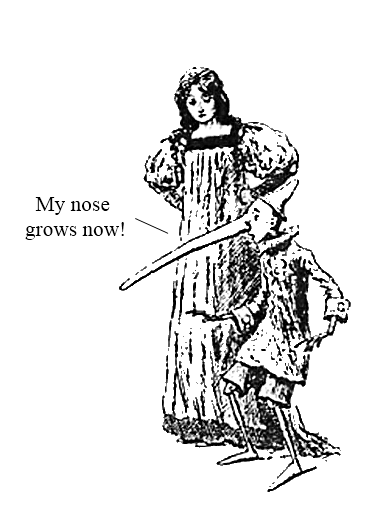
\includegraphics[height=30ex]{res/Pinocchio_paradox.png}
  \caption{Pinocchio says a lie and stretches his nose}
  \label{fig:Pinocchio}
\end{figure}

\begin{thm}
    The halting problem is undecidable.
\end{thm}
\begin{proof}
    Assume there exists a Turing machine $\mathbb B$ that decides the
    halting problem i.e.~for all Turing machines $\mathbb A$ and all
    strings $x$

    \[ \mathbb B(\enc{\mathbb A}, x) =
    \begin{cases}
      \one  & \text{if } \mathbb A \text{ halts on } x\\
      \zer  & \text{if } \mathbb A \text{ does not halt on } x
    \end{cases}\]

    Now using $\mathbb B$ construct a Turing machine $\mathbb B'$ that
    simulates $\mathbb B(\enc{\mathbb A}, \enc{\mathbb A})$ on its input
    $\enc{\mathbb A}$ and enters an infinite loop if
    $\mathbb B(\enc{\mathbb A}, \enc{\mathbb A}) = \zer$. Expressed more
    formally this means

    \[
      \mathbb B' \text{ halts on } \enc{\mathbb A} ⇔
      \mathbb A \text{ does not halts on } \enc{\mathbb A}.
    \]

    Setting $\mathbb A = \mathbb B'$ yields the desired contradiction.
\end{proof}

For a more detailed proof of this fact and lot more information on computability
see \cite{Cooper2004}. As the halting problem is undecidable the halting set
defined by
\[
 \mathcal{K} = \set{⟨\enc{\mathbb A}, x⟩ \mid \mathbb A \text{ halts on } x}
\]
is undecidable. However using the universal Turing machine it is clearly
semi-decidable.


\section{Prerequisites from model theory}
% !TEX encoding = UTF-8
% !TEX TS-program = xelatex
% !TEX spellcheck = en_GB
% !TEX engine = xelatex
% !TEX root = ../Herbstrith-H10_over_AI.tex
%
% ███    ███  ██████  ██████  ███████ ██          ████████ ██   ██
% ████  ████ ██    ██ ██   ██ ██      ██             ██    ██   ██
% ██ ████ ██ ██    ██ ██   ██ █████   ██             ██    ███████
% ██  ██  ██ ██    ██ ██   ██ ██      ██             ██    ██   ██
% ██      ██  ██████  ██████  ███████ ███████        ██    ██   ██ ██

The idea of model theory is to differentiate between the statements we can make
about mathematical objects and the implementation of these mathematical objects.
We will define \emph{languages} and their syntax and will describe what it means
for a mathematical object to \emph{model a theory}. In this section I will
closely follow Chapter 1 of the textbook~\cite{Marker2002}.

\subsection{Formulae and models}
% ███████  ██████  ██████  ███    ███ ██    ██ ██       █████  ███████
% ██      ██    ██ ██   ██ ████  ████ ██    ██ ██      ██   ██ ██
% █████   ██    ██ ██████  ██ ████ ██ ██    ██ ██      ███████ █████
% ██      ██    ██ ██   ██ ██  ██  ██ ██    ██ ██      ██   ██ ██
% ██       ██████  ██   ██ ██      ██  ██████  ███████ ██   ██ ███████

Informally, a first-order formula is just a string of symbols that signify
distinguished constants, functions, and relations. We demand that a formula is
well-behaved according to the interpretability of constants, functions, and
relations. We do however not make any assumptions on the implementation of these
symbols. So a formula captures the \emph{syntax} of a collection of mathematical
objects. A model, on the other hand, describes the \emph{semantics} of an
object. It gives concrete interpretations of the symbols of a language and tells
us, how the formulae are to be understood.

\begin{defin}
  A \emph{language} \(\lang\) is a quadruple \((\mathcal{F}, \mathcal{R},
  \mathcal{C}, ar: \mathcal{F} ∪ \mathcal{R} → ℕ \setminus \set{0})\), where
  \(\mathcal{F}\) is a set of function symbols, \(\mathcal{R}\) is a set of
  relation symbols, and \(\mathcal{C}\) is a set of constant symbols, such that
  all of these sets are pair-wise disjoint. The function \(ar: \mathcal{F} ∪
  \mathcal{R} → ℕ\) assigns to every function symbol \(f ∈ \mathcal{F}\) and
  every relation symbol \(R ∈ \mathcal{R}\) the \emph{arity} \(n_f\) or \(n_R\)
  respectively.
\end{defin}

By the the arity \(n_f\) of a function symbol \(f\) we describe that \(f\)
should eventually be interpreted as a function on \(n_f\) variables.
Analogously, the arity \(n_R\) of a relation symbol \(R\) describes that \(R\)
will denote an \(n_R\)-ary relation.

It is customary to denote the language \(\lang = (\mathcal{F}, \mathcal{R},
\mathcal{C}, ar: \mathcal{F} ∪ \mathcal{R} → ℕ \setminus \set{0})\) by
\[
  \lang = \set{f ∈ \mathcal{F}; R ∈ \mathcal{R}; c ∈ \mathcal{C}}
\]
and thereby drop the arity function from the notation.

\begin{exam}
  Examples of languages include
  \begin{exlist}
    \item the language of pure sets \(\lang = ∅\);

    \item the language of (reflexive) orderings \(\lang_{≤} =
    \set{\mathtt{≤}}\), where \(≤\) is a binary relation symbol;

    \item the language of groups \(\lang_{group} = \set{\mathtt{\cdot, {}^{-1};
    e}}\), where \(\mathtt{\cdot}\) is a binary function symbol,
    \(\mathtt{{}^{-1}}\) is an unary function symbol, and \(\mathtt{e}\) is a
    constant; and

    \item the language of rings with unity \(\lang_{ring} = \set{\mathtt{+, -,
    \cdot; 0, 1}}\), where \(\mathtt{+, -}\), and \(\mathtt{\cdot}\) are binary
    function symbols and \(\mathtt{0, 1}\) are constants.
  \end{exlist}
\end{exam}

These languages allow for various interpretations---not all of them might be the
intended ones---and each of these interpretations is called a model. More
formally, we have the following definition.

\begin{defin}
  Let \(\lang = \set{f ∈ \mathcal{F}; R ∈ \mathcal{R}; c ∈ \mathcal{C}}\) be a
  language. A \emph{model} \(\mathfrak{A}\) of \(\lang\) is a non-empty set
  \(A\), called the \emph{universe} or \emph{carrier set} of \(\mathfrak{A}\),
  together with
  \begin{thmlist}
    \item a function \(f^{\mathfrak{A}}: A^{n_f} → A\) for every function symbol
    \(f ∈ \mathcal{F}\),

    \item a relation \(R^{\mathfrak{A}} \subseteq A^{n_R}\) for every relation
    symbol \(R ∈ \mathcal{R}\), and

    \item a constant \(c^{\mathfrak{A}} ∈ A\) for every constant symbol \(c ∈
    \mathcal{C}\).
  \end{thmlist}
  We will use the notation
  \[
    {\mathfrak{A}} = ⟨A; f^{\mathfrak{A}} ∈ \mathcal{F}; R^{\mathfrak{A}} ∈
      \mathcal{R}; c^{\mathfrak{A}} ∈ \mathcal{C}⟩
  \]
  to denote this model.

  A model in a language without relation symbols is called \emph{algebraic
  structure}.
\end{defin}

\begin{exam}
  We list some examples of models for the languages defined above.
  \begin{exlist}
    \item In the language of pure sets \(\lang = ∅\), every non-empty set \(S\)
    gives rise to a model \(\mathfrak{S} = ⟨S⟩\).

    \item An example of a model in the language of (reflexive) orderings
    \(\lang_{≤} = \set{\mathtt{≤}}\) is \(\mathfrak{N}_{≤} := ⟨ℕ, ≤⟩\), where
    \(≤\) denotes the usual ordering of the non-negative integers.

    \item As for \(\lang_{group} = \set{\mathtt{\cdot, {}^{-1}; e}}\), any group
    \(G\) induces a model. Indeed, consider the algebraic structure
    \(\mathfrak{G} := ⟨G; \cdot^{\mathfrak{G}},
    {\mathtt{{}^{-1}}}^{\mathfrak{G}}; \mathtt{e}^{\mathfrak{G}}⟩\), where
    \(\cdot^{\mathfrak{G}}\) denotes the binary group-operation,
    \({\mathtt{{}^{-1}}}^{\mathfrak{G}}\) denotes inversion, and
    \(\mathtt{e}^{\mathfrak{G}} ∈ G\) is the neutral element of \(G\). However,
    \(\mathfrak{N}_{sg} = ⟨ℕ; +, \mathbf{0}; 0⟩\), where \(\mathbf{0}: ℕ → ℕ\)
    is defined by \(n ↦ 0\) for all \(n ∈ ℕ\), is an \(\lang_{group}\)-structure
    as well.

    \item Let \(R\) be a ring with unity, then \(\mathfrak{R} := ⟨R;
    \mathtt{+^{\mathfrak{R}}, -^{\mathfrak{R}}, \cdot^{\mathfrak{R}};
    0^{\mathfrak{R}}, 1^{\mathfrak{R}}}⟩\), where \(\mathtt{+^{\mathfrak{R}},
    -^{\mathfrak{R}}, \cdot^{\mathfrak{R}}}\) are the respective binary
    ring-operations and \(\mathtt{0^{\mathfrak{R}}, 1^{\mathfrak{R}}}\) are the
    neutral elements with respect to addition and multiplication, is a model in
    \(\lang_{ring}\). Of special interest to us will be the
    \(\lang_{ring}\)-structures \(\mathfrak{Z} := ⟨ ℤ; +, -, \cdot; 0, 1⟩\)
    denoting the structure of rational integers and \(\mathfrak{O}_K :=
    ⟨\algint; +, -, \cdot; 0, 1⟩\) denoting the structure of algebraic integers
    (cf.~\cref{sec:number theory}). However, we will also consider the
    \(\lang_{ring}\)-structure \(\mathfrak{N} := ⟨ℕ; +, \dotminus, \cdot; 0,
    1⟩\) of the non-negative integers, where \(\dotminus: ℕ \times ℕ → ℕ\) is
    defined by \(n \dotminus m = \max(0, n - m)\).
  \end{exlist}
\end{exam}

As a next step we want to define the syntax of formulae but at first we consider
terms.

\begin{defin}
  Let \(\lang = \set{f ∈ \mathcal{F}; R ∈ \mathcal{R}; c ∈ \mathcal{C}}\) be a
  language. The set of \emph{\(\lang\)-terms} is the smallest set \(T(\lang)\),
  such that
  \begin{thmlist}
    \item every constant symbol \(c ∈ \mathcal{C}\) is a term,

    \item every variable symbol \(\mathtt{x_1, x_2, x_3, …}\) is a term, and

    \item if \(\seq[n_f]{t} ∈ T(\lang)\) are terms then \(f(\seq[n_f]{t})\) is a
    term for all function symbols \(f ∈ \mathcal{F}\).
  \end{thmlist}
\end{defin}

For example \(\mathtt{+(+(\cdot(x_1, x_1), \cdot(x_2, x_2)), 1)}\) is an
\(\lang_{ring}\) term. It is more conventional---and more legible---to write
this term in infix-notation to obtain the ‘polynomial’
\[
  \mathtt{x_1 \cdot x_1 + x_2 \cdot x_2 + 1},
\]
Using the very important technique of \emph{structural induction}, we
can show that every term in an \(\lang_{ring}\)-structure is a polynomial
(see~\cref{lem:terms of rings are polynomials}). In order to do this we need to
consider terms as functions. There is just a little technicality in our way,
that can be avoided by defining \(S^{0} := \set{∅}\) for every set \(S\) and
interpreting a constant \(c\) as a \(0\)-ary function \(c : S^{0} → S\).

\begin{defin}
  Let \(\lang := \set{f ∈ \mathcal{F}; R ∈ \mathcal{R}; c ∈ \mathcal{C}}\) be a
  language and let \(\mathfrak{A}\) be a model of \(\lang\) with universe \(A\).
  For a term \(t(\mathtt{\seq{x}}) ∈ T(\lang)\) that contains at most the
  variables \(\mathtt{\seq{x}}\) we define the \emph{term function}
  \(t^{\mathfrak{A}}: A^n → A\) associated to \(t(\mathtt{\seq{x}})\)
  recursively as follows:
  \begin{thmlist}
    \item If \(t(\mathtt{\seq{x}}) = c ∈ \mathcal{C}\), then
    \(t^{\mathfrak{A}}(\seq{α}) = c^{\mathfrak{A}}\) for all \(\seq{α} ∈ A\).

    % \item If \(t(\mathtt{\seq{x}}) = f(\mathtt{x_{i_1}, … x_{i_{n_f}}})\) for
    % some \(f ∈ \mathcal{F}\) and some \(\set{\seq[n_f]{i}} \subseteq \set{1, …,
    % n_f}\), then
    % \[
    %   t^{\mathfrak{A}}(\seq{α}) := f^{\mathfrak{A}}(α_{i_1}, …, α_{i_{n_f}})
    % \]
    % for all \(\seq{α} ∈ A\).

    \item If \(t(\mathtt{\seq{x}}) = \mathtt{x_i}\) for \(1 ≤ i ≤ n\), then
    \(t^{\mathfrak{A}} := π_{i}^n\) is the projection onto the \(i\)-th
    coordinate.

    \item If \(t(\mathtt{\seq{x}})\) is of the form
    \[
      t(\mathtt{\seq{x}}) = f(t_1(\mathtt{\seq{x}}), …,
      t_{n_f}(\mathtt{\seq{x}}))
    \]
    for some basic function \(f ∈ \mathcal{F}\) and some terms
    \(t_1(\mathtt{\seq{x}}), …, t_{n_f}(\mathtt{\seq{x}})\), then
    \[
      t^{\mathfrak{A}}(\seq{α}) := f^{\mathfrak{A}}(t_1^{\mathfrak{A}}(\seq{α}),
      …, t_{n_f}^{\mathfrak{A}}(\seq{α})).
    \]
  \end{thmlist}
\end{defin}

In other words, the set of term functions of a given model \(\mathfrak{A}\) is
the smallest set of functions, that contains all projections, all constants, as
well as all basic functions of \(\mathfrak{A}\), and is closed under
composition. If \(\mathfrak{A}\) is an algebraic structure, the set of term
functions of \(\mathfrak{A}\) is sometimes called the \emph{function clone} of
\(\mathfrak{A}\).

\begin{lem}\label{lem:terms of rings are polynomials}
  Let \(R\) be a ring with unity and \(\mathfrak{R}\) its associated
  \(\lang_{ring}\)-structure. The set of term functions of \(\mathfrak{R}\) is
  the set of polynomial functions with integral coefficients \(ℤ[X_1, X_2, …]\).
\end{lem}
\begin{proof}
  Let \(t ∈ T(\lang_{ring})\) be a term. We argue by structural induction, that
  is induction on the number of symbols appearing in \(t\).
  \begin{plist}
    \item If \(t = c\) is a constant, then \(t = \zer\) or \(\one\). Both are
    constant polynomials with integral coefficients.

    \item If \(t = \mathtt{x_i}\) for some \(i ∈ ℕ \setminus \set{0}\), then
    \(t^{\mathfrak{R}} = X_i\) is a monomial.

    \item Finally, if \(t = f(t_1, t_2)\), where \(f ∈ \set{+, -, \cdot}\) and
    \(t_1, t_2\) are terms, then we can assume that \(t_1^{\mathfrak{R}}\) and
    \(t_2^{\mathfrak{R}}\) are polynomials with integral coefficients and as
    \(ℤ[X_1, X_2, …]\) is closed under sums, differences and products of
    polynomials, the term functions are indeed contained in \(ℤ[X_1, X_2, …]\)
  \end{plist}

  To see the converse inclusion note that every positive integer \(n\) can be
  expressed as the \(\lang_{ring}\)-term
  \[
    \underbrace{\mathtt{1 + 1 + … + 1}}_{n\text{-times}}
  \]
  and every non-positive integer \(n\) can be expressed as
  \[
    \mathtt{0 -} \underbrace{\mathtt{1 - 1 - … - 1}}_{|n|\text{-times}}.
  \]
  Then a monomial \(a X_{i_1} … X_{i_d} ∈ ℤ[X_1, X_2, …]\), with \(i_1,…,i_d ∈
  ℕ \setminus \set{0}\) not necessarily distinct, can be expressed as the term
  \[
    \mathtt{a} \cdot x_{i_1} \cdot … \cdot x_{i_d},
  \]
  where \(\mathtt{a}\) is the term representing the integer \(a\). Finally,
  since every polynomial \(p\) is a finite sum of monomials \(p = m_1 + … +
  m_k\) we can find a term
  \[
    t = \mathtt{m_1 + … + m_k},
  \]
  where \(\mathtt{m_i}\) is the term representing \(m_i\) (\(1 ≤ i ≤ k\)), such
  that \(t^{\mathfrak{R}} = p\).
\end{proof}

In the lemma above I have considered the polynomial functions
\[
  p_1 : R → R, \; p_1(X_1) := X_1^2 + 1 \quad \text{and} \quad
  p_2 : R^2 → R, \; p_2(X_1, X_2) := X_1^2 + 1
\]
as the same polynomial function. This can be justified by identifying all
polynomials in the ring \(ℤ[X_1, X_2, …]\) with functions \(p: R^ℕ → R\)
depending only on finitely many arguments.

Finally, we have all tools at hand to formally define formulae in a language.

\begin{defin}
  Let \(\lang := \set{f ∈ \mathcal{F}; R ∈ \mathcal{R}; c ∈ \mathcal{C}}\) be a
  language. We call a string \(ϕ\) \emph{atomic \(\lang\)-formula} if
  \begin{thmlist}
    \item there exist \(\lang\)-terms \(t_1, t_2\) such that \(ϕ = t_1 \doteq
    t_2\), or%
    \footnote{Note the difference between the two symbols \(=\) and \(\doteq\)
    in this equation. While \(=\) denotes an equality on the meta-level, i.e.\
    it denotes that both strings contain the same symbols in the same order,
    \(\doteq\) is just a symbol contained in the strings.}

    \item there exist \(\lang\)-terms \(t_1, …, t_{n_R}\) and a relation symbol
    \(R ∈ \mathcal{R}\) such that \(ϕ = R(t_1, …, t_{n_R})\).
  \end{thmlist}

  The set of \emph{formulae} in \(\lang\) is the smallest set \(Φ(\lang)\)
  containing all atomic \(\lang\)-formulae that is closed under the following
  constructions:
  \begin{thmlist}[resume]
    \item If \(ϕ ∈ Φ(\lang)\) is a formula, so is its \emph{negation} \(¬ϕ ∈
    Φ(\lang)\).

    \item If \(ϕ_1, ϕ_2 ∈ Φ(\lang)\) are formulae, then their \emph{conjunction}
    \((ϕ_1 ∧ ϕ_2) ∈ Φ(\lang)\) is a formula.

    \item If \(ϕ(x) ∈ Φ(\lang) \) is a formula containing at least the
    variable \(x\) in one of its terms, then \(∃ x :
    ϕ(x) ∈ Φ(\lang)\) is a formula.
  \end{thmlist}

    Just for convenience we define the following abbreviations:
    \begin{thmlist}[resume]
      \item If \(ϕ_1, ϕ_2 ∈ Φ(\lang)\) are formulae, we define their
      \emph{disjunction} \((ϕ_1 ∨ ϕ_2)\) by \(¬(¬ϕ_1 ∧ ¬ϕ_2)\).

      \item If \(ϕ_1, ϕ_2 ∈ Φ(\lang)\) are formulae, then \(ϕ_1 → ϕ_2\) is short
      for \(¬(ϕ_1 ∧ ¬ ϕ_2)\).

      \item If \(ϕ(x) ∈ Φ(\lang)\) is a formula containing at least the
      variable \(x\), then we abbreviate \(¬ ∃ x: ¬
      ϕ(x)\) by \(∀ x: ϕ(x)\).
    \end{thmlist}
\end{defin}

Note that formulae as defined above are just strings and do not inherit any
meaning or truthfulness.%
\footnote{Note however, that there are formulae that are true in all models, for
instance \(\mathtt{∀ x_1 : x_1 \doteq x_1}\) is easily seen to hold in all
models.}
However, once we interpret a formula in a model, we can say whether the formula
is true or false. Let us consider some examples in the language \(\lang_{ring}\)
of rings with
one.

\begin{exam}
  The following are \(\lang_{ring}\)-formulae:
  \begin{exlist}
    \item \(\mathtt{x_1 \cdot x_2 \doteq x_3}\)
    \item \(\mathtt{∃ x_2 : x_1 \cdot x_2 \doteq 1}\)
    \item\label{ex:formula distributivity}
     \(\mathtt{∀x_1 : ∀x_2 : ∀x_3 : (x_1 + x_2) \cdot x_3 \doteq x_1 \cdot x_3 + x_2 \cdot x_3}\)
  \end{exlist}
  Intuitively, the formulae above can be interpreted as
  \begin{exlist}
    \item \(\mathtt{x_1}\) times \(\mathtt{x_2}\) equals \(\mathtt{x_3}\),
    \item \(\mathtt{x_1}\) is invertible with inverse \(\mathtt{x_2}\), and
    \item the ring operations satisfy the distributivity condition.
  \end{exlist}
\end{exam}

In the formulae of the previous example one technical obstacle becomes apparent.
While the formula of \cref{ex:formula distributivity} is either true or false in
a given \(\lang_{ring}\)-structure, the formulae in (1) and (2) depend on the
choice of elements for \(\mathtt{x_1, x_2}\) and \(\mathtt{x_3}\). For this
reason we must distinguish between two kinds of appearances of variables.

\begin{defin}
  Let \(x\) be a variable and let \(ϕ\) be a formula containing \(x\). If \(ϕ\)
  contains \(∃ x : ψ(x)\) as a sub-formula for some formula \(ψ\), we call this
  appearance of \(x\) \emph{bound appearance}. All appearances of \(x\) that are
  not of this shape are called \emph{free appearances}.
\end{defin}

In \cref{ex:formula distributivity} all appearances of \(\mathtt{x_1, x_2}\) and
\(\mathtt{x_3}\) are bound. In (2) variable \(\mathtt{x_2}\) appears bound\-ed
while \(\mathtt{x_1}\) is free and in (1) all variables appear freely. For a
formula \(ϕ\) we will write \(ϕ(\mathtt{\seq{x}})\) to emphasize that at most
the variables \(\mathtt{\seq{x}}\) appear freely in \(ϕ\).

\begin{defin}
  Let \(\lang\) be a language and let \(\mathfrak{A}\) be model of \(\lang\)
  with universe \(A\). For a formula \(ϕ = ϕ(\mathtt{\seq{x}})\) and elements
  \(\seq{α} ∈ A\) we say that \(ϕ(\seq{α})\) is \emph{true} in \(\mathfrak{A}\)
  or \(\mathfrak{A}\) \emph{models} \(ϕ(\seq{α})\) and write
  \[
    \mathfrak{A} \models ϕ(\seq{α})
  \]
  if the following recursively defined conditions are met:
  \begin{thmlist}
    \item If \(ϕ = t_1 \doteq t_2\) for two terms \(t_1, t_2\), then
    \(\mathfrak{A} \models ϕ(\seq{α})\) if
    \[
      t_1^{\mathfrak{A}}(\seq{α}) = t_2^{\mathfrak{A}}(\seq{α}).
    \]

    \item If \(ϕ = R(t_1, …, t_{n_R})\) for a relation symbol \(R\) and terms
    \(t_1, …, t_{n_R}\), then \(\mathfrak{A} \models ϕ(\seq{α})\) if
    \[
      R^{\mathfrak{A}}(t_1^{\mathfrak{A}}(\seq{α}), …,
       t_{n_R}^{\mathfrak{A}}(\seq{α})).
    \]

    \item If \(ϕ = ¬ ψ\) for a formula \(ψ\), then \(\mathfrak{A} \models
    ϕ(\seq{α})\) if \(\mathfrak{A} \models ψ(\seq{α})\) does not hold.

    \item If \(ϕ = (ψ_1 ∧ ψ_2)\) for two formulae \(ψ_1, ψ_2\), then
    \(\mathfrak{A} \models ϕ(\seq{α})\) if both \(\mathfrak{A} \models
    ψ_1(\seq{α})\) and \(\mathfrak{A} \models ψ_2(\seq{α})\) hold.

    \item If \(ϕ(\mathtt{\seq{x}}) = ∃ x : ψ(x, \mathtt{\seq{x}})\),
    then \(\mathfrak{A} \models ϕ(\seq{α})\) if there exists an \(α ∈ A\) such
    that \(\mathfrak{A} \models ψ(α, \seq{α})\).
  \end{thmlist}
\end{defin}

\begin{rem}
  \begin{exlist}
    \item I leave it as an exercise to check that our abbreviations \(∨, →\)
    and \(∀\) have their intended interpretation of \emph{disjunction},
    \emph{implication} and \emph{universal quantification}.

    \item Note that variables can have both free \emph{and} bound appearances in
    the same formula, for example \(\mathtt{x_2}\) in
    \[
      \mathtt{(∃ x_2 : x_1 \cdot x_2 \doteq x_2) ∧ (x_2 + x_3 \doteq x_1)}.
    \]
    By the definition of what it means that a formula is true in a model, we can
    restrict our attention to formulae, such that all variables appear
    \emph{either} freely \emph{or} bounded but not both, and if a variable
    appears bound, then it is bound by a single quantifier. For instance, it is
    easy to check that the formula above is true in a model if and only if the
    following formula is true
    \[
      \mathtt{(∃ x_2 : x_1 \cdot x_2 \doteq x_2) ∧ (x_4 + x_3 \doteq x_1)}.
    \]
    Variables that appear freely in a formula are also called \emph{free
    variables.}
  \end{exlist}
\end{rem}

A formula without free variables is called a \emph{sentence}. In a fixed model a
sentence is either true or false. This follows easily form the definition of
truth in a model.

\subsection{Morphisms, theories, and decidability}\label{sec:theories}
% ████████ ██   ██ ███████  ██████  ██████  ██ ███████ ███████
%    ██    ██   ██ ██      ██    ██ ██   ██ ██ ██      ██
%    ██    ███████ █████   ██    ██ ██████  ██ █████   ███████
%    ██    ██   ██ ██      ██    ██ ██   ██ ██ ██           ██
%    ██    ██   ██ ███████  ██████  ██   ██ ██ ███████ ███████

In this section I introduce some very important notions from model theory and
universal algebra. I start with the concept of \emph{morphism}. The reader
should already have encountered morphisms in basic lectures on abstract algebra.
They are just mappings that respect the basic operations of structures. More
formally, one defines a morphism as follows.

\begin{defin}
  Let \(\lang := \set{f ∈ \mathcal{F}; R ∈ \mathcal{R}; c ∈ \mathcal{C}}\) be a
  language and \(\mathfrak{A}, \mathfrak{B}\) two models in \(\lang\) with
  universes \(A\) and \(B\) respectively. A function \(φ : A → B\) is called
  \emph{\(\lang\)-morphism} if
  \begin{thmlist}
    \item \(φ(f^{\mathfrak{A}}(\seq[n_f]{α})) = f^{\mathfrak{B}}(φ(α_1), …,
    φ(α_{n_f}))\) holds for all \(f ∈ \mathcal{F}\) and all \(\seq[n_f]{α} ∈
    A\);

    \item \(R^{\mathfrak{A}} (\seq[n_R]{α})\) implies
    \(R^{\mathfrak{B}}(φ(α_1), …, φ(α_{n_r}))\) for all \(R ∈ \mathcal{R}\) and
    all \(\seq[n_R]{α} ∈ A\); and

    \item \(φ(c^{\mathfrak{A}}) = c^{\mathfrak{B}}\) for all \(c ∈
    \mathcal{C}\).
  \end{thmlist}
\end{defin}

\begin{rem}
  \begin{exlist}
    \item   Despite the similarity of the definition of
    \(\lang_{ring}\)-morphisms to ring-morphisms in the sense of abstract
    algebra, not every \(\lang_{ring}\)-morphism is a ring-morphism and vice
    versa. Consider for example the identity \(\mathrm{id}_ℕ\) on the
    \(\lang_{ring}\)-structure \(\mathfrak{N}\). As \(ℕ\) is not a ring in the
    sense of abstract algebra, \(\mathrm{id}_ℕ\) is not a ring-morphism, but it
    is clearly an \(\lang_{ring}\)-morphism.

    On the other hand, the mapping \(φ: ℤ → ℤ \times ℤ\) defined by
    \[
      φ(α) = (0, α)
    \]
    is a ring-morphism that is not an \(\lang_{ring}\)-morphism, as \(1\) is not
    mapped to the neutral element \((1, 1)\) in \(ℤ \times ℤ\).

    \item As in abstract algebra, an injective morphism is called
    \emph{monomorphism}, a surjective one \emph{epimorphism}, and a bijective
    morphism is called \emph{isomorphism}.
  \end{exlist}
\end{rem}

\begin{defin}
  Let \(\lang\) be a language.
  \begin{thmlist}
    \item A set of \(\lang\)-sentences is called an \emph{\(\lang\)-theory}.

    \item Let \(\mathfrak{A}\) be a model in \(\lang\). We say \(\mathfrak{A}\)
    satisfies a theory \(T\) and write \(\mathfrak{A} \models T\) if
    \(\mathfrak{A}\) models all sentences in \(T\).

    \item A class of models \(\mathcal{M}\) in \(\lang\) is called
    \emph{elementary class} if there exists an \(\lang\)-theory \(T\) such that
    for all models
    \(\mathfrak{A}\) the following equivalence holds
    \[
      \mathfrak{A} ∈ \mathcal{M} \quad ⇔ \quad \mathfrak{A} \models T.
    \]

    \item An elementary class \(\mathcal{V}\) of algebraic structures is called
    \emph{universal variety} if the defining theory \(T\) does only include
    universally quantified atomic formulae.
  \end{thmlist}
\end{defin}

\begin{exam}
  The class of groups forms a universal variety with respect to
  \(\lang_{group}\). This is the case since the group axioms
  \begin{align*}
     \mathtt{∀ x_1 } & \mathtt{: x_1 \cdot e \doteq x_1},\\
     \mathtt{∀ x_1 } & \mathtt{: e \cdot x_1 \doteq x_1},\\
     \mathtt{∀ x_1 } & \mathtt{: ∀ x_2 : ∀ x_3 :
             (x_1 \cdot x_2) \cdot x_3 \doteq x_1 \cdot (x_2 \cdot x_3)},\\
     \mathtt{∀ x_1 } & \mathtt{: x_1 \cdot x_1^{-1} \doteq e}, \text{ and}\\
     \mathtt{∀ x_1 } & \mathtt{: x_1^{-1} \cdot x_1 \doteq e}
  \end{align*}
  characterize groups completely. Another example of a universal variety are
  rings with unity. Note however, that fields do not form a universal variety
  with respect to \(\lang_{ring}\), as we demand that elements unequal to \(0\)
  are invertible which can be expressed by the sentence
  \[
    \mathtt{∀ x_1 : (¬ x_1 \doteq 0) → (∃ x_2 : x_1 \cdot x_2 \doteq 1)}
  \]
  containing both universal and existential quantifiers.
\end{exam}

Universal varieties are useful, as substructures can be characterized by
embeddings, e.g.\ we have that a subset \(S\) of a ring with unity \(R\) is a
sub-ring if and only if \(S\) carries an \(\lang_{ring}\)-structure
\(\mathfrak{S}\) such that the embedding
\[
  ι: S → R, \quad ι(α) = α
\]
is an \(\lang_{ring}\)-morphism between \(\mathfrak{S}\) and the
\(\lang_{ring}\)-structure of \(R\). Moreover, we have the following
important result.

\begin{thm}\label{thm:elementary equivalence}
  Let \(\mathfrak{A}\) and \(\mathfrak{B}\) be two \(\lang\)-structures, with
  universe \(A\) and \(B\) respectively, and let \(φ: A → B\) be a bijective
  \(\lang\)-morphism. Then \(\mathfrak{A}\) and \(\mathfrak{B}\) are
  \emph{elementary equivalent}, i.e.\ for all \(\lang\)-sentences
  \(ϕ\), \(\mathfrak{A}\) models \(ϕ\) if and only if \(\mathfrak{B}\) models
  \(ϕ\).
\end{thm}

A proof of the theorem using induction on the structure of formulae can be found
in the textbook~\cite[Thm~1.1.10]{Marker2002}. For the reader who wants to learn
more about universal algebra the textbook~\cite{Burris1981} is an excellent
reference.

To conclude this section we describe theories of special importance to our task
of settling Hilbert's tenth problem and define what it means to decide a theory.

\begin{defin}
  Let \(\lang\) be a language and let \(\mathfrak{A}\) be a model with universe
  \(A\) in \(\lang\).
  \begin{thmlist}
    \item The \emph{full theory of \(\mathfrak{A}\)} is the set
    \[
      \mathtt{Th}(\mathfrak{A}) :=
        \set{ϕ ∈ Φ(\lang) : ϕ \text{ is a sentence and }\mathfrak{A} \models ϕ}
    \]
    of all sentences true in \(\mathfrak{A}\).

    \item The \emph{purely Diophantine theory of \(\mathfrak{A}\)} is the set
    \[
      \mathtt{H10}^*(\mathfrak{A}) :=
        \set{ϕ ∈ Φ(\lang) \mid
        ϕ = \mathtt{∃ x_{i_1} : … ∃ x_{i_k} : }ψ(\mathtt{x_{i_1}, …, x_{i_k}}),
        ψ \text{ is atomic, and } \mathfrak{A} \models ϕ}
    \]
    of all fully existentially quantified atomic formulae that are satisfied by
    \(\mathfrak{A}\).

    \item The \emph{primitive positive theory of \(\mathfrak{A}\)} is the set
    \[
      \mathtt{Th}_{∃+}(\mathfrak{A}) :=
        \set{ϕ ∈ Φ(\lang) \;\middle\vert \substack{
          {ϕ = \mathtt{∃ x_{i_1} : … ∃ x_{i_k} : }
          \bigwedge_{j = 1}^m ψ_j(\mathtt{x_{i_1}, …, x_{i_k}}),}\\
        {ψ_j \text{ is atomic for } 1 ≤ j ≤ m
        \text{, and } \mathfrak{A} \models ϕ}}}
    \]
    of all fully existentially quantified conjunctions of atomic formulae that
    are satisfied by \(\mathfrak{A}\).
  \end{thmlist}
\end{defin}

Let us take a look at some examples to get a better understanding of these
abstract definitions.

\begin{exam}
  \begin{exlist}
    \item Let \(\mathfrak{Q} := ⟨ℚ; +, -, \cdot; 0, 1⟩\) be the
    \(\lang_{ring}\)-structure of the rationals. Then
    \[
      \mathfrak{Q} \models
        \mathtt{∀ x_1 : (¬ x_1 \doteq 0) → (∃ x_2 : x_1 \cdot x_2 \doteq 1)}
    \]
    and therefore this sentence is contained in \(\mathtt{Th}(\mathfrak{Q})\).
    However, \(2 ∈ ℤ \setminus \set{0}\) is not invertible in \(ℤ\). Thus, the
    sentence is not in \(\mathtt{Th}(\mathfrak{Z})\).

    \item Consider \(ϕ := \mathtt{∃ x_1 : x_1^2 + 1 \doteq 0}\). Then \(ϕ\) can
    be satisfied by the witness \(i ∈ ℂ\) in \(\mathfrak{C} := ⟨ ℂ; +, -, \cdot;
    0, 1⟩\) as \(i^2 + 1 = 0\) holds in \(\mathfrak{C}\). Thus, \(ϕ\) is
    contained in \(\mathtt{H10}^*(\mathfrak{C})\), but the sentence is not
    contained in \(\mathtt{H10}^*(\mathfrak{Z})\).

    \item Consider the directed graph \(\mathfrak{G} := ⟨\set{1, 2, 3, 4}; E⟩\)
    below.
    \begin{center}
      \includegraphics{res/digraph}
    \end{center}
    Here \(E\) denotes the binary adjacency relation, where for instance \(E(1,
    2)\) holds but \(E(2, 1)\) does not. The following sentence intuitively says
    that a graph contains a cycle of length \(3\).
    \[
      ϕ := \mathtt{∃ x_1 : ∃ x_2 : ∃ x_3 :
           (E(x_1, x_2) ∧ E(x_2, x_3) ∧ E(x_3, x_1))}
    \]
    Using \(1\) as witness for \(\mathtt{x_1}\) and \(2, 4\) as witnesses for
    \(\mathtt{x_2}, \mathtt{x_3}\), we obtain that \(ϕ\) is contained in
    \(\mathtt{Th}_{∃+}(\mathfrak{G})\), and it is not difficult to find a
    directed graph that does not model \(ϕ\).
  \end{exlist}
\end{exam}

While we can already state a lot of properties in the languages we have
considered so far, we can for instance not formulate a sentence in the language
\(\lang_{ring}\) that says a specific polynomial has a root. Take for instance
the \(\lang_{ring}\)-structure \(\mathfrak{C}\) of \(ℂ\), we cannot formulate a
sentence that says the polynomial \(X^2 - i ∈ ℂ[X]\) has a root in \(ℂ\). To
get around this limitation we define \emph{diagrams}.
\begin{defin}
  Let \(\lang\) be a language and \(\mathfrak{A}\) a model in \(\lang\) with
  universe \(A\). We define the \(A\)-language as
  \[
    \lang_A := \lang ∪ \set{\mathtt{c}_a \mid a ∈ A}
  \]
  the union of \(\lang\) and a constant symbol for each element of \(A\).
\end{defin}

Clearly, \(\mathfrak{A}\) is also a model in \(\lang_A\) by additionally
interpreting \(\mathtt{c}_a^{\mathfrak{A}} := a\) for all \(a ∈ A\).

\begin{defin}
  Let \(\lang\) be a language and let \(\mathfrak{A}\) be a model with universe
  \(A\) in \(\lang\). We define the following \(\lang_A\)-theories.
  \begin{thmlist}
    \item The \emph{complete diagram} of \(\mathfrak{A}\) is the set
    \[
      D^c(\mathfrak{A}) :=
        \set{ϕ ∈ Φ(\lang_A) \mid ϕ \text{ is a sentence and }
        \mathfrak{A} \models ϕ}
    \]
    of all \(\lang_A\)-sentences true in \(\mathfrak{A}\).

    \item The \emph{Diophantine theory} of \(\mathfrak{A}\) is the set
    \[
      \mathtt{H10}(\mathfrak{A}) :=
        \set{ϕ ∈ Φ(\lang_A) \mid
        ϕ = \mathtt{∃ x_{i_1} : … ∃ x_{i_k} : }ψ(\mathtt{x_{i_1}, …, x_{i_k}}),
        ψ \text{ is atomic, and } \mathfrak{A} \models ϕ}
    \]
    of all fully existentially quantified atomic \(\lang_A\)-formulae that are
    satisfied by \(\mathfrak{A}\).

    \item The \emph{primitive positive diagram} of \(\mathfrak{A}\) is the set
    \[
      D_{∃+}(\mathfrak{A}) :=
        \set{ϕ ∈ Φ(\lang) \;\middle\vert\; \substack{
          {ϕ = \mathtt{∃ x_{i_1} : … ∃ x_{i_k} : }
          \bigwedge_{j = 1}^m ψ_j(\mathtt{x_{i_1}, …, x_{i_k}}),}\\
        {ψ_j \text{ is atomic for } 1 ≤ j ≤ m
        \text{, and } \mathfrak{A} \models ϕ}}}
    \]
    of all full existentially quantified conjunctions of atomic
    \(\lang_A\)-formulae that are satisfied by \(\mathfrak{A}\).

    \item The \emph{atomic diagram} of \(\mathfrak{A}\) is the set
    \[
      D(\mathfrak{A}) :=
        \set{ϕ ∈ Φ(\lang_A) \;\middle\vert\; \substack{
          {\text{there exists an atomic formula } ψ \text{ with }}\\
          {ϕ = ψ \text{, or } ϕ = ¬ ψ \text{ and }
           \mathfrak{A} \models ϕ}}
        }
    \]
    of all atomic \(\lang_A\)-sentences and negations of atomic
    \(\lang_A\)-sentences that are satisfied by \(\mathfrak{A}\).
  \end{thmlist}
\end{defin}

Of special interest to us is the Diophantine theory of rings with unity. The
name can be justified by the following lemma.

\begin{thm}\label{thm:Diophantine theory}
  Let \(R\) be a ring with unity and let \(\mathfrak{R}\) be its
  \(\lang_{ring}\)-structure.
  \begin{thmlist}
    \item The set of term functions associated to \(\lang_R\)-terms is the set
    of polynomial functions \(R[X_1, X_2, …]\).

    \item Let \(\mathtt{P} \subseteq Φ(\lang_R)\) be the set of all
    existentially quantified atomic \(\lang_R\)-formulae. There exists a
    surjection
    \[
      π: \mathtt{P} → R[X_1, X_2, …]
    \]
    such that for all sentences \(ϕ ∈ \mathtt{P}\) we have
    \[
      ϕ ∈ \mathtt{H10}(\mathfrak{R}) \quad ⇔ \quad
      π(ϕ) \text{ has roots in } R.
    \]
  \end{thmlist}
\end{thm}
\begin{proof}
  \begin{plist}
    \item Let \(t\) be an \(\lang_R\)-term. One proves completely analogously to
    the proof of \cref{lem:terms of rings are polynomials}, that
    \(t^{\mathfrak{R}} ∈ R[X_1, X_2, …]\) is a polynomial function. The only
    difference is that constants now range over all of \(R\) instead of
    \(\set{0, 1}\) thus yielding the different coefficients.

    To see the converse inclusion we note that monomials \(α X_{i_1} … X_{i_d} ∈
    R[X_1, X_2, …]\), with indices \(\seq[d]{i} ∈ ℕ \setminus \set{0}\)
    not necessarily distinct, correspond to terms
    \[
      \mathtt{c}_α \cdot \mathtt{x_{i_1} \cdot … \cdot x_{i_d}}.
    \]
    Since every polynomial \(p\) is a finite sum of monomials we obtain a term
    representing \(p\) by joining the terms representing the monomials using the
    symbol \(\mathtt{+}\).

    \item Let \(ϕ ∈ \mathtt{P}\) be a sentence. By definition of \(\mathtt{P}\)
    there exists an atomic \(\lang_{R}\)-formula \(ψ\) such that
    \[
      ϕ = \mathtt{∃ x_{i_1} : … ∃ x_{i_k} : } ψ(\mathtt{x_{i_1}, …, x_{i_k}}).
    \]
    Since \(\lang_{R}\) contains no relation symbols, all atomic
    \(\lang_{R}\)-formulae are identities of terms. Thus, there exist terms
    \(t_1, t_2\) such that
    \[
      ψ = t_1 \doteq t_2.
    \]
    By part (i) of the theorem, the term functions \(t_1^{\mathfrak{R}}\) and
    \(t_2^{\mathfrak{R}}\) are polynomial functions in \(R[X_1, X_2, …]\). We
    set \(π(ϕ) := t_1^{\mathfrak{R}} - t_2^{\mathfrak{R}}\).

    To see that \(π\) is surjective let \(p ∈ R[X_1, X_2, …]\) be a polynomial.
    Then by (i) there exists a term \(t\) such that \(t^{\mathfrak{R}} = p\).
    Now set
    \[
      ϕ := \mathtt{∃ x_{i_1} : … ∃ x_{i_k} : } t(\mathtt{x_{i_1}, …, x_{i_k})
        \doteq 0},
    \]
    where \(\mathtt{x_{i_1}, …, x_{i_k}}\) are all variable symbols appearing in
    \(t\). Then \(π(ϕ) = p\) as claimed.

    Let now \(ϕ ∈ \mathtt{H10}(\mathfrak{R})\) be a sentence that is true in
    \(\mathfrak{R}\). By the discussion above we find that
    \[
      ϕ := \mathtt{∃ x_{i_1} : … ∃ x_{i_k} : }
        t_1(\mathtt{x_{i_1}, …, x_{i_k}}) \doteq
        t_2(\mathtt{x_{i_1}, …, x_{i_k}}),
    \]
    for some \(\lang_R\)-terms \(t_1, t_2\). Using the definition of truth in a
    model this is the case if and only if there exist elements \(α_{i_1}, …,
    α_{i_k} ∈ R\) such that
    \[
      t_1^{\mathfrak{R}}(α_{i_1}, …, α_{i_k}) =
      t_2^{\mathfrak{R}}(α_{i_1}, …, α_{i_k}).
    \]
    But this identity holds if and only if \(π(ϕ) = t_1 - t_2\) has roots in
    \(R\).
  \end{plist}
\end{proof}

To finish our last task of this section we have to overcome once more a
technical difficulty: If we want to define what it means to \emph{decide} a
theory, we must identify the theory with subsets of \(ω\). To this end,
\textcite{Goedel1931} introduced a method that is today commonly known as
\emph{Gödelization}.

\begin{defin}
  Let \(\lang\) be an at most countable language and let
  \[
    i: \lang ∪ \set{\doteq, \mathtt{¬, ∧, ∃, :, (, ), x, '}}
    → ℕ \setminus \set{0}
  \]
  be an injective function such that \(i(s) > 9\) for all \(s ∈ \lang\) and the
  image of \(i\) is an initial segment of the usual order of \(ℕ \setminus
  \set{0}\).

  The \emph{Gödel number} \(\mathrm{gn}(ϕ)\) of a formula \(ϕ ∈ Φ(\lang)\) is
  obtained by first replacing every variable symbol \(\mathtt{x_j}\) in \(ϕ\) by
  the string
  \[
    \mathtt{x}\overbrace{\mathtt{'…'}}^{j\text{-times}}.
  \]
  Say the resulting string is
  \[
    \mathbf{s} = s_1 s_2 … s_n,
  \]
  where \(s_i\) is a symbol contained in \(\lang ∪ \set{\doteq, \mathtt{¬, ∧,
  ∃, (, ), x, '}}\) then
  \[
    \mathrm{gn}(ϕ) := p_1^{i(s_1)} p_2^{i(s_2)} … p_n^{i(s_n)},
  \]
  where \(p_i ∈ ℕ\) is the \(i\)-th prime.
\end{defin}

By the uniqueness of the prime factorization in \(ℕ\), two different formulae
cannot have the same Gödel number. Finally, one obtains an encoding
\(\enc{\cdot}: Φ(\lang) → ω\) by composing \(\mathrm{gn}\) with an encoding of
the natural numbers (see~\cref{ex:omega encoding}).

\begin{exam}
To get a feeling for how fast the Gödel numbers grow let us consider the
Gödelization of the following \(\lang_{ring}\)-formula
\[
  \mathtt{∃ x_1 : x_1 \doteq 0}.
\]
We choose the function \(i\) as described in the table below.
\[
  \begin{array}{l @{\qquad} r r r r r r r r r r r r r r}
    \toprule
    s & \doteq & ¬ & ∧ & ∃ & : & ( & ) & \mathtt{x} & ' & + & - & \cdot & \mathtt{0} & \mathtt{1}\\
    i(s) & 1 & 2 & 3 & 4 & 5 & 6 & 7 & 8 & 9 & 10 & 11 & 12 & 13 & 14\\
    \bottomrule
  \end{array}
\]
Using the notation from the definition we obtain
\[
  \mathbf{s} = ∃ x' : x' \doteq 0
\]
yielding the Gödel number
\begin{align*}
  \mathrm{gn}(ϕ) &= 2^4 3^8 5^9 7^5 11^8 13^9 17^1 19^{13},
\end{align*}
which already has \(52\) decimal digits.
\end{exam}

\begin{defin}
  Let \(\lang\) be an at most countable language. An \(\lang\)-theory \(T\) is
  \emph{decidable} (\emph{semi-decidable}) if the set
  \[
    \set{\enc{ϕ} : ϕ ∈ T}
  \]
  is decidable (semi-decidable).
\end{defin}

\begin{figure}
  \includegraphics[scale=1]{res/theories}
  \caption{The theories defined in \cref{sec:theories} may be ordered by
  set-inclusion (arrows pointing from sub- to super-sets) and many-one
  reducibility}
  \label{fig:theories}
\end{figure}

\begin{rem}
  Let \(\mathfrak{A}\) be a model. If one orders the theories defined above with
  respect to set-inclusion, the interrelations depicted in \cref{fig:theories}
  hold.

  If the language and the universe of \(\mathfrak{A}\) are at most countable
  then we can Gödelize these theories and identify them with their set of Gödel
  numbers. In this setting it is not hard to see that the theories
  \begin{itemize}
    \item \(
      S(\mathtt{Th}(\mathfrak{A})) :=
      \set{ϕ ∈ Φ(\lang) \mid ϕ \text{ is a sentence}}
    \),

    \item \(
      S(\mathtt{H10}^*(\mathfrak{A})) :=
        \set{ϕ ∈ Φ(\lang) \mid
        ϕ = \mathtt{∃ x_{i_1} : … ∃ x_{i_k} : }ψ(\mathtt{x_{i_1}, …, x_{i_k}}),
        ψ \text{ is atomic}}
    \)

    \item \(
      S(\mathtt{Th}_{∃+}(\mathfrak{A})) :=
        \set{ϕ ∈ Φ(\lang) \;\middle\vert \substack{
          {ϕ = \mathtt{∃ x_{i_1} : … ∃ x_{i_k} : }
          \bigwedge_{j = 1}^m ψ_j(\mathtt{x_{i_1}, …, x_{i_k}}),}\\
        {ψ_j \text{ is atomic for } 1 ≤ j ≤ m}}}
    \)

    \item \(S(D^c(\mathfrak{A})) :=
      \set{ϕ ∈ Φ(\lang_A) \mid ϕ \text{ is a sentence}}\),

    \item \(S(\mathtt{H10}(\mathfrak{A})) :=
        \set{ϕ ∈ Φ(\lang_A) \mid
        ϕ = \mathtt{∃ x_{i_1} : … ∃ x_{i_k} : }ψ(\mathtt{x_{i_1}, …, x_{i_k}}),
        ψ \text{ is atomic}}\),

    \item \(S(D_{∃+}(\mathfrak{A})) :=
        \set{ϕ ∈ Φ(\lang) \;\middle\vert\; \substack{
          {ϕ = \mathtt{∃ x_{i_1} : … ∃ x_{i_k} : }
          \bigwedge_{j = 1}^m ψ_j(\mathtt{x_{i_1}, …, x_{i_k}}),}\\
        {ψ_j \text{ is atomic for } 1 ≤ j ≤ m}}}\), and


    \item \(S(D(\mathfrak{A})) :=
        \set{ϕ ∈ Φ(\lang_A) \;\middle\vert\; \substack{
          {\text{there exists an atomic formula } ψ \text{ with }}\\
          {ϕ = ψ \text{, or } ϕ = ¬ ψ}}
        }\)
  \end{itemize}
  are decidable. A Turing machine deciding
  these theories must only check whether a string encodes a syntactically valid
  sentence using the allowed symbols \cite[cf.][Chap.~8.1]{Cooper2004}.

  Let now \(T ∈ \set{\mathtt{Th}(\mathfrak{A}), \mathtt{H10}^*(\mathfrak{A}),
  \mathtt{Th}_{∃+}(\mathfrak{A}), D^c(\mathfrak{A}), \mathtt{H10}(\mathfrak{A}),
  D_{∃+}(\mathfrak{A}), D(\mathfrak{A})}\) be a theory and \(U \subseteq T\) a
  subtheory contained in \(\set{\mathtt{Th}(\mathfrak{A}),
  \mathtt{H10}^*(\mathfrak{A}), \mathtt{Th}_{∃+}(\mathfrak{A}),
  D^c(\mathfrak{A}), \mathtt{H10}(\mathfrak{A}), D_{∃+}(\mathfrak{A}),
  D(\mathfrak{A})}\). We prove that \(U ≤_m T\) holds. For this purpose note
  that \(U = T ∩ S(U)\) holds and consider the sentence
  \[
    ϕ_{⊥} := \mathtt{0 \doteq 1},
  \]
  which is contained in \(S(T)\) but not in \(T\). The function \(f: ω → ω\)
  defined by
  \[
    f(x) :=
    \begin{cases}
      x & \text{if } x ∈ \enc{S(U)}\\
      \enc{ϕ_{⊥}} & \text{otherwise}
    \end{cases}
  \]
  is computable, as \(S(U)\) is decidable. Additionally, it has the property
  that a string \(x\) is contained in \(\enc{U}\) if and only if \(f(x)\) is
  contained in \(T\). Indeed if \(x\) encodes a sentence \(ϕ\) that is part of
  \(S(U)\) then \(f(x) = x\). In this case, \(x\) is in \(T\) if and only if
  \(x\) is in \(S(U) ∩ T = U\). If on the other hand \(x\) is not in
  \(\enc{S(U)}\) then \(x\) is surely not contained in \(\enc{U}\) and \(f(x) =
  \enc{ϕ_{⊥}}\) which is not turn contained in \(\enc{T}\). Thus proving the
  claim.

  Concerning rings of algebraic integers (incl. \(ℤ\)) and their models
  \(\modalgint\), we will see in \cref{lem:intersections and unions} that
  \(\mathtt{Th}_{∃+}(\modalgint)\) is many-one reducible to
  \(\mathtt{H10}^*(\modalgint)\) and that \(D_{∃+}(\modalgint)\) is many-one
  reducible to \(\mathtt{H10}^*(\modalgint)\) In order to settle Hilbert's tenth
  problem we will show for some rings of algebraic integers that the halting set
  \(\mathcal{K}\) is many-one reducible to \(D_{∃+}(\modalgint)\) and vice
  versa. However, even more is true as we will show that this is sufficient for
  the interrelations---with respect to many-one reducibility---depicted in
  \cref{fig:theories 2} to hold between the theories.
\end{rem}

\begin{figure}
  \includegraphics[scale=1]{res/theories_2}
  \caption{For models of algebraic integers \(\modalgint\) the diagram collapses
  w.r.t. many-one reducibility if \(\mathcal{K} <_m D_{∃+}(\modalgint)\)}
  \label{fig:theories 2}
\end{figure}

\subsection{Computable structures and decidable models}%
\label{sec:computable structures}
%  ██████  ██████  ███    ███ ██████      ███████ ████████ ██████
% ██      ██    ██ ████  ████ ██   ██     ██         ██    ██   ██
% ██      ██    ██ ██ ████ ██ ██████      ███████    ██    ██████
% ██      ██    ██ ██  ██  ██ ██               ██    ██    ██   ██
%  ██████  ██████  ██      ██ ██ ██       ███████    ██    ██   ██ ██

Up to this point the encoding of problems was treated as some kind of black-box.
This subsection takes a categorical view on computability and ensures us,
that---up to a sensible definition---encodings of the rings we concern ourselves
with do not matter. The interested reader may whish to consult the excellent
textbook by \textcite{Stoltenberg1999} on this subject. However, I am using the
notation of the paper~\cite{Khoussainov2000} and the
textbook~\cite[Chap.~16]{Cooper2004}.

Throughout this section I will identify the set of non-negative integers \(ℕ\)
with the set of strings \(ω\) via the encoding described in \cref{ex:omega
encoding}.

\begin{defin}
  Let \(\lang\) be an at most countable language. We say \(\lang\) is
  \emph{computable} if we can Gödelize the set of \(\lang\)-formulae
  \(Φ(\lang)\) in such a way, that \(\gn(Φ(\lang))\) is decidable.
\end{defin}

Note that we can only change the function \(i\) described in the definition of
the Gödelization. Thus, we can rearrange the symbols of our language to simplify
our computations. In this view, a language \(\lang = \set{f ∈ \mathcal{F}; R ∈
\mathcal{R}; c ∈ \mathcal{C}}\) is computable if we can encode its basic symbols
in such a way that
\begin{enumerate}
  \item the sets \(i(\mathcal{F})\), \(i(\mathcal{R})\), and
  \(i(\mathcal{C})\) are decidable; and

  \item the function \(\mathtt{ar}: i(\mathcal{F}) ∪ i(\mathcal{R}) → ω\)
  defined by \(i(ℓ) ↦ \ar(ℓ)\) is computable.
\end{enumerate}
Indeed, if this is the case, we can use the properties of the Gödelization to
obtain from an encoded formula \(\gn(ϕ)\) the sequence of symbols that \(ϕ\)
contains and then check efficiently using structural induction, whether \(ϕ\) is
a well-formed formula.

\begin{lem}\label{lem:properties of Goedelization}
  Let \(\lang\) be a computable language. For a fixed Gödelization, the
  following numbers are computable for every \(\lang\)-formula \(ϕ\) from the
  Gödel number \(\gn(ϕ)\).
  \begin{thmlist}
    \item The length \(\ln(ϕ)\) of \(ϕ\), which is the number of symbols
    appearing in \(ϕ\).

    \item For every \(i ∈ \set{1, …, \ln(ϕ)}\), the code \(i(s)\) of the symbol
    \(s\) appearing in the \(i\)-th position of \(ϕ\).

    \item The number of quantifiers appearing in \(ϕ\) and the number of free
    variables.

    \item The Gödel number of the negation of \(ϕ\).

    \item If a second formula \(ψ\) is given, one can efficiently obtain the
    Gödel number of the conjunction of \(ϕ\) and \(ψ\).

    \item If \(ϕ(x)\) contains the free variable \(x\) and
    the Gödel number of a term \(t\) is given, one can efficiently obtain the
    Gödel number of \(ϕ(t)\), i.e.\ the Gödel number of the formula, where each
    free appearance of \(x\) is replaced by \(t\).
  \end{thmlist}
\end{lem}

The lemma is easily proven using that the prime factorization of a positive
integer is computable. All of the numbers above can then be computed by
manipulating the factorizations.

Of course, all languages we will consider---and have considered so far---are
computable. In fact, they are all either finite, or contain only finitely many
non-constant symbols.

\begin{defin}
  Let \(\lang\) be a computable language and let \(i: \lang → ℕ\) be the
  function used to Gödelize \(\lang\).
  \begin{thmlist}
    \item A model \(\mathfrak{A}\) in \(\lang\), with universe \(A \subseteq
    ω\), is called \emph{computable} if \(A\) is decidable and there exist two
    computable functions \(\mathtt{F}, \mathtt{C}\) and a decidable relation
    \(\mathtt{R}\) such that
    \[
      \mathtt{F}(i(f), ⟨\seq[n_f]{α}⟩) = f^{\mathfrak{A}}(\seq[n_f]{α})
    \]
    holds for all function symbols \(f ∈ \mathcal{F}\) and all elements
    \(\seq[n_f]{α} ∈ A\),
    \[
      \mathtt{R}(i(R), ⟨\seq[n_R]{α}⟩) \quad ⇔ \quad
      R^{\mathfrak{A}}(\seq[n_R]{α})
    \]
    holds for all relation symbols \(R ∈ \mathcal{R}\) and all elements
    \(\seq[n_R]{α} ∈ A\), and
    \[
      \mathtt{C}(i(c)) = c^{\mathfrak{A}}
    \]
    holds for all constant symbols \(c ∈ \mathcal{C}\). As before angled
    brackets \(⟨\cdot⟩\) in the expressions above indicate pairings like in
    \cref{ex:total pairing}.

    \item A model \(\mathfrak{A}\) with universe \(A\) is called
    \emph{efficiently presentable} if \(\mathfrak{A}\) is isomorphic to a
    computable model with universe \(Ω_A ⊂ ω\) in the same language.

    \item A morphism between computable models is called \emph{computable
    morphism} if it is computable as a partial function.
  \end{thmlist}
\end{defin}

\begin{rem}
  \begin{exlist}
    \item An efficient presentation of a ring \(R\) is a ring-homomorphism
    \(\enc{\cdot}: R → Ω_R\) of \(R\), where \(Ω_R \subseteq ω\) is decidable
    and all operations of \(Ω_R\) are computable functions.

    \item \Textcite{Stoltenberg1999} use a slightly modified definition of
    computable rings. They consider \emph{effective enumerations} \(α_R : Ω_R →
    R\), where \(Ω_R \subseteq ω\) is a computable \(\lang_{ring}\)-structure in
    the sense of the definition above and \(α_R\) is an
    \(\lang_{ring}\)-epimorphism. Then the ring \(R\) is called computable if
    there exists an effective enumeration \(α_R : Ω_R → R\) such that the
    equivalence relation
    \[
      x_1 \equiv_{α_R} x_2  \quad ⇔ \quad
      α_R(x_1) = α_R(x_2)
    \]
    is decidable on \(Ω_R\).

    This definition can have slight technical advantages. But note that in this
    case \(Ω_R\) need not be a ring in the sense of abstract algebra, an
    \(\lang_{ring}\)-structure in the sense of universal algebra suffices. Let
    \(\lfloor α_R^{-1}(\set{η}) \rfloor ∈ Ω_R\) denote the smallest element of
    \(α_R^{-1}(\set{η})\) in lexicographic order. By setting \(\enc{η} = \lfloor
    α_R^{-1}(\set{η}) \rfloor\) for each \(η ∈ R\) one obtains a
    ring-isomorphism \(R → Ω_R\) that gives rise to an efficient presentation of
    \(R\). So \(R\) is computable in the sense of \textcite{Stoltenberg1999} if
    and only if it is efficiently presentable in the sense of this thesis.
  \end{exlist}
\end{rem}

The following alternative characterization of efficiently presentable models can
easily be proven via structural induction.

\begin{lem}
  Let \(\lang\) be an at most countable language and \(\mathfrak{A}\) a model in
  \(\lang\) with universe \(A\). Then the following are equivalent.
  \begin{thmlist}
    \item \(\mathfrak{A}\) is efficiently presentable as a model in \(\lang\).
    \item \(\mathfrak{A}\) is efficiently presentable as a model in \(\lang_A\).
    \item The atomic diagram of \(\mathfrak{A}\) is decidable.
  \end{thmlist}
\end{lem}

\begin{exam}
  \begin{exlist}
    \item Every finite structure \(⟨S; f_1, …, f_n⟩\) with \(S \subseteq ω\) is
    computable. The set \(S\) is decidable as it is finite and the domain of
    each operation \(f_i\) for \(1 ≤ i ≤ n\) is finite as well. A Turing machine
    computing \(f_i\) can store the images of all elements in the domain in
    memory.

    \item In \cref{ex:tally encoding} the non-negative integer \(n\) was encoded
    by a string of \(n\) consecutive \(\one\)-s. I have also already presented
    the algorithm deciding \(\enc{ℕ} \subseteq ω\) with respect to this
    encoding. Considering \(ℕ\) as an \(\lang_{ring}\)-structure, one finds that
    the tally encoding gives rise to an efficient presentation of \(ℕ\).

    The constants \(0\) and \(1\) are trivially computable, by clearing the tape
    in the first case and writing a single \(\one\) in the second case. Using
    the pairing function of \cref{ex:tally pairing} the binary operations
    \(+\), \(\dotminus\), and \(\cdot\) are also easily seen to be computable.
    As for \(+\) the algorithm takes the input
    \[
      \one … \one \zer \one … \one
    \]
    and replaces the \(\zer\)-symbol by an \(\one\) and deletes the rightmost
    \(\one\).

    \item \label{ex:polynomials are computable} If \(R\) is a computable
    integral domain, then the polynomial algebras \(R[X_1, …, X_n]\) in
    arbitrary many indeterminates and \(R[X_1, X_2, …]\) in countably many
    indeterminates are efficiently presentable \(R\)-algebras.

    A possible implementation starts by implementing the monoid \(⟨M; \cdot; X_i
    \mid i ∈ ℕ⟩\) and extends it to the \(R\)-algebra \(R[X_1, X_2, …]\). Within
    \(R[X_1, X_2, …]\) the domain of every subalgebra \(R[X_1, …, X_n]\) is
    decidable and therefore the structure is computable. See the
    textbook~\cite[Sec.~4.4]{Stoltenberg1999} for a more detailed discussion and
    \cref{app:polynomials} for a sample implementation based on this idea.

    \item\label{ex:Z is computable}
    In general \(ℤ\) and every finitely generated free \(ℤ\)-algebra viewed as
    \(\lang_{ring}\)-structure is efficiently presentable. As for integers, one
    extends the presentation of \(ℕ\) by a sign-bit.

    To present free \(ℤ\)-algebras one uses a basis, say \(ξ_1, …, ξ_n\). Then
    any element \(η\) can be encoded as an \(n\)-tuple of integers. Addition and
    subtraction are defined coordinate-wise. To implement the multiplication one
    stores the finite multiplication table of the basis elements
    \[
      \begin{array}{l @{\qquad} r r r r}
        \toprule
              & ξ_1   & ξ_2     & … & ξ_n     \\
        \midrule
        ξ_1 & ξ_1^2     & ξ_1 ξ_2 & … & ξ_1 ξ_n \\
        ξ_2 & ξ_2 ξ_1   & ξ_2^2   & … & ξ_2 ξ_n \\
        \vdots & \vdots &  \vdots & \ddots  & \vdots  \\
         ξ_n & ξ_n ξ_1  & ξ_n ξ_2 & … & ξ_n^2\\
        \bottomrule
      \end{array}
    \]
    in memory and extends it to all of the \(ℤ\)-algebra linearly.

    \item \(⟨ℕ, ≤⟩\) is efficiently presentable using the tally encoding and
    \(n ≤ m\) if and only if \(n \dotminus m = 0\). So deciding \(n ≤ m\) boils
    down to applying floor subtraction and checking whether the tape is empty.
    Both operations are clearly computable.
  \end{exlist}
\end{exam}

It is a natural question whether two efficient presentations of the same model
are computably isomorphic, i.e.\ if there exists a computable isomorphism
between them. We will see that the last example differs from the others in this
regard. But before studying computable isomorphisms we need a lemma.

\begin{lem}
  Let \(f: Q → Q'\) be a computable bijection between two decidable problems
  \(Q, Q' ⊂ ω\). Then the inverse mapping \(f^{-1}: Q' → Q\) is computable as
  well.
\end{lem}
\begin{proof}
  Let \(x ∈ Q'\) be given. To find \(f^{-1}(x)\) one lists all elements of \(ω\)
  and checks for every \(y ∈ ω\) whether \(y\) is contained in \(Q\). Since \(Q\)
  is decidable, this can be carried out efficiently. If \(y\) is not
  contained in \(Q\), we try the next element in \(ω\). Otherwise, we compute
  \(f(y)\) and check whether \(f(y) = x\) holds. In this case, we set
  \(f^{-1}(x) := y\) and are finished. If \(f(y)\) does not equal \(x\) we take
  the next element of \(ω\) and start over. The process will stop at some point
  as \(f\) is surjective.
\end{proof}

\begin{defin}
  Let \(\lang\) be a computable language. A model is called \emph{computably
  categorical} if it is efficiently presentable and every pair of efficient
  presentations is computably isomorphic.
\end{defin}

In the case of rings of algebraic integers (see~\cref{cor:O K is computable})
the following theorem applies and assures us that the decidability of
\textsc{H10} does in fact not depend on the encoding chosen.

\begin{thm}\label{thm:computable categoricity}
  Let \(R\) be a finitely generated, efficiently representable ring. Then \(R\)
  is computably categorical.
\end{thm}

This theorem follows from a more general result of \textcite{Malcev1961}. The
idea of the proof is to let \(ξ_1, …, ξ_n ∈ R\) be a set of generators of \(R\)
over \(R\) and let \(φ_1: R → R_1, φ_2: R → R_2\) be the efficient
representations of \(R\) together with the respective ring isomorphisms. Then
\(φ_1(ξ_1), …, φ_1(ξ_n)\) generate \(R_1\) over \(R_1\) and \(φ_2(ξ_1), …,
φ_2(ξ_n)\) generate \(R_2\) over \(R_2\). Storing these finitely many values of
the isomorphism \(φ_2 \circ φ_1^{-1}\) in memory one can use the computability
of \(R_1\) and \(R_2\) respectively to extend the partial mapping in a natural
way.

As for the decidability of \textsc{H10} over some ring of algebraic integers
\(\algint\) this means, that if we have two encodings of \(\algint\) that allow
to evaluate polynomial expressions, then we can efficiently transform a
statement in one encoding into a statement in the other encoding and vice versa.

\begin{exam}\label{ex:N is computably categorical}
  Another example of a computably categorical structure is \(\struc{N}\), the
  \(\lang_{ring}\)-structure of \(ℕ\). To see this let \(\struc{N}_1\) and
  \(\struc{N}_2\) be two computable representations of \(ℕ\). A computable
  isomorphism \(f\) between the two structures can be obtained by defining
  \(f(\mathtt{0}^{\struc{N}_1}) := \mathtt{0}^{\struc{N}_2}\) and then
  recursively
  \[
    f(\mathtt{c_{n + 1}}^{\struc{N}_1}) := f(\mathtt{c_n}^{\struc{N}_1}) +
    \mathtt{1}^{\struc{N}_2},
  \]
  where \(\mathtt{c_{n}}\) is as before the constant representing the integer
  \(n\).
\end{exam}

Note however, that there are structures where the choice of presentation
matters. In fact, \(⟨ℕ, ≤⟩\) is not computably categorical. A proof using the
undecidability of the halting problem can be found in the
paper~\cite[Prob.~1.6]{Shore}.

\begin{lem}\label{lem:H10 is semi decidable}
  Let \(R\) be a computable, commutative ring with unity and \(\mathfrak{R}\)
  its \(\lang_{ring}\)-structure. Then the Diophantine theory
  \(\mathtt{H10}(\mathfrak{R})\) is semi-decidable.
\end{lem}
\begin{proof}
  Since \(R\) is computable, \(\lang_{R}\) is computable and as a consequence
  the set of (Gödel numbers of) fully existentially quantified atomic
  \(\lang_{R}\)-formulae is decidable.

  Let now \(ϕ = \mathtt{∃ x_1: … : ∃ x_n :} ψ(\mathtt{\seq{x}})\) be a fully
  existentially quantified \(\lang_{R}\)-formula. By \cref{thm:Diophantine
  theory} there exists a polynomial \(p ∈ R[\seq{X}]\) such that for all
  \(\seq{α} ∈ R\) we have that
  \[
    \mathfrak{R} \models ψ(\seq{α}) \quad ⇔ \quad
    p(\seq{α}) = 0.
  \]
  In fact, the polynomial \(p\) can be obtained from the Gödel number \(\gn(ϕ)\)
  efficiently. Thus, the relation \(H ⊂ ω^2\) defined by
  \[
    H(\gn(ϕ), ⟨\seq{α}⟩) \quad :⇔ \quad
    p(\seq{α}) = 0
  \]
  is computable and the Diophantine theory \(\mathtt{H10}(\mathfrak{R})\) is
  semi-decidable by \cref{pro:characterizations of ce sets}.
\end{proof}


\section{Prerequisites from number theory}\label{sec:number theory}
% !TEX encoding = UTF-8
% !TEX TS-program = xelatex
% !TEX spellcheck = en_GB
% !TEX engine = xelatex
% !TEX root = ../Herbstrith-H10_over_AI.tex
%
% ███    ██ ██    ██ ███    ███ ██████  ███████ ██████      ████████ ██   ██
% ████   ██ ██    ██ ████  ████ ██   ██ ██      ██   ██        ██    ██   ██
% ██ ██  ██ ██    ██ ██ ████ ██ ██████  █████   ██████         ██    ███████
% ██  ██ ██ ██    ██ ██  ██  ██ ██   ██ ██      ██   ██        ██    ██   ██
% ██   ████  ██████  ██      ██ ██████  ███████ ██   ██        ██    ██   ██ ██

\subsection{Number fields and rings of algebraic integers}
% ███    ██ ██    ██ ███    ███        ███████ ██      ██████  ███████
% ████   ██ ██    ██ ████  ████        ██      ██      ██   ██ ██
% ██ ██  ██ ██    ██ ██ ████ ██        █████   ██      ██   ██ ███████
% ██  ██ ██ ██    ██ ██  ██  ██        ██      ██      ██   ██      ██
% ██   ████  ██████  ██      ██ ██     ██      ███████ ██████  ███████

In this section I will closely follow Chapter 1 of the German
textbook~\cite{Neukirch2006}. However, the content is also present in the
English reference~\cite[Chap.~2]{Milne2017}, and sometimes the presentation of
this reference will be recited. We start with a series of definitions and remind
the reader on some important results from algebraic number theory and
commutative algebra. But at first let us fix an important notation.

Let \(R\) and \(S\) be commutative rings with unity. Let \(φ: R → S\) be a
ring-homomorphism mapping \(1_R\) to \(1_S\), then \(S\) is called an
\emph{\(R\)-algebra} and we write \(a α\) as a short form for \(φ(a) \cdot α\)
(\(a ∈ R\) and \(α ∈ S\)). We are especially interested in the case
where \(R \subseteq S\) and \(φ\) is chosen to be the embedding of \(R\) into
\(S\). In this situation we denote  by \(R[\seq{α}]\) the smallest ring inside
\(S\) containing \(R\) and all \(\seq{α} ∈ S\). Then \(R[\seq{α}]\) contains all
polynomial expressions in \(\seq{α}\) with coefficients in \(R\), i.e.\ all
elements of the form
\[
  \sum_{(\seq{i}) ∈ ℕ^n} a_{i_1, …, i_n} α^{i_1} … α^{i_n},
\]
where only finitely many \(a_{i_1, …, i_n} ∈ R\) are non-zero.

\begin{defin}
  A finite field-extension \(K\) of the rationals \(ℚ\) is called
  \emph{algebraic number field}. This means that \(K\) is a field and at the
  same time a \(ℚ\)-algebra, that is finite-dimensional viewed as a \(ℚ\)-vector
  space. The \emph{degree} \([K : ℚ]\) is the dimension of \(K\) viewed as a
  \(ℚ\)-vector space.
\end{defin}

For convenience we will always assume that \(K\) is a subset of the complex
pane \(ℂ\).

\begin{exam}
  \begin{exlist}
    \item \(ℚ\) is (up to isomorphism) the only algebraic number field of
    degree \(1\).

    \item \(ℚ[√2] = \set{a + b √2 : a, b ∈ ℚ}\) is an algebraic number field
    of degree \(2\). The inverse of \(a + b √2\), where not both \(a\) and \(b\)
    are \(0\), is given by \(\frac{a - b √2}{a^2 - 2 b^2}\).

    \item \(ℚ[√[3]{2}] = \set{a + b √[3]{2} + c √[3]{4} : a, b ∈ ℚ}\) is an
    algebraic number field of degree \(3\).
  \end{exlist}
\end{exam}

If \(K\) is a number field, then the extension \(K/M\) of number fields is in
fact an \emph{algebraic} one. This means that every \(x ∈ K\) is the root of
some polynomial with coefficients in \(M\). We denote by \(μ_{M, x} ∈ M[X]\) the
monic polynomial with root \(x\) dividing (in \(M[X]\)) all other polynomials
with root \(x\). The polynomial \(μ_{M, x}\) is called \emph{minimal polynomial}
of \(x\) over \(M\). By the minimality condition (w.r.t.\ divisibility in
\(K[X]\)) on \(μ_{M, x}\) this polynomial must be irreducible.

In fact, every element \(x\) in \(K\) is algebraic over the rationals \(ℚ\).
Note that the field of all algebraic elements \(\overline{ℚ}\)---called
\emph{algebraic closure} of \(ℚ\)---is however not a number field, as the
extension \(\overline{ℚ} / ℚ\) is (countably) infinite.

\begin{defin}
  Let \(R ⊂ S\) be commutative rings with unity. Then \(α ∈ S\) is called
  \emph{integral} over \(R\) if it is the root of a monic polynomial with
  coefficients in \(R\), i.e.\ if \(α\) satisfies an equation of the form
  \[
    α^n + a_{n-1}α^{n - 1} + … + a_0 = 0
  \]
  for some \(n ≥ 1\) and some \(\seq[n - 1]{a} ∈ R\). If all elements of \(S\)
  are integral over \(R\) then \(S\) is called \emph{integral} over \(R\). If
  \(R\) is an integral domain then \(R\) is \emph{integrally closed} if for all
  elements \(x ∈ \Quot(R)\) being integral over \(R\) implies \(x ∈ R\).
\end{defin}

Of course, when one wants to use tools from algebra some structure on the
considered sets is needed. Thus, the following theorem, implying that if \(α, β
∈ S\) are algebraic over \(S\), so are their sum and product, is very desirable.

\begin{thm}\label{thm:integral closure}
  Let \(R \subseteq S\) be commutative rings with unity. Then the elements of
  \(S\) that are integral over \(R\) form a subring of \(S\).
\end{thm}

Richard Dedekind gave a proof of this theorem using the following proposition.

\begin{pro}\label{pro:characterization of integral elements}
  Let \(R \subseteq S\) be commutative rings with unity. Then \(α ∈ S\) is
  integral over \(R\) if and only if there exists a finitely generated
  \(R\)-module \(M \subseteq S\) such that \(αM \subseteq M\), in fact \(M =
  R[α]\) can be chosen.
\end{pro}

\begin{proof}[Proof of \cref{thm:integral closure}]
  Let \(α, β ∈ S\) be integral over \(R\) and let \(M\) and \(N\) be finitely
  generated \(R\)-modules contained in \(S\) such that \(αM \subseteq M\) and
  \(βN \subseteq N\) hold. We define the product of the two modules as
  \[
    MN := \set{\sum_{i=1}^k m_i n_i \;\middle\vert\;
     k ∈ ℕ, \seq[k]{m} ∈ M, \seq[k]{n} ∈ N}.
  \]
  Clearly, \(MN\) contains \(0\) as \(M\) (and \(N\)) contains \(0\).
  Furthermore, it is closed under addition, and the inverse of an element in
  \(MN\) can be found by inverting all \(m_i ∈ M\) (or \(n_i ∈ N\)) in the sum.
  Thus, \(MN\) forms a subgroup of \(S\). Note that \(a m_i\) is contained in
  \(M\) for all \(a ∈ R\) and \(m_i ∈ M\) since \(M\) is an \(R\)-module. As a
  consequence,
  \[
    a \sum_{i=1}^k m_i n_i = \sum_{i=1}^k \underbrace{a m_i}_{∈ M} n_i
  \]
  is contained in \(MN\) for all \(a ∈ R\) and all \(\seq[k]{m} ∈ M\),
  \(\seq[k]{n} ∈ N\), and we can deduce that \(MN\) is an \(R\)-module.

  Let \(\set{\seq[m]{e}} \subseteq M\) generate \(M\) and \(\set{\seq[n]{f}}
  \subseteq N\) generate \(N\). Then it is easily seen that the finite set
  \[
    \set{e_i f_j : 1 ≤ i ≤ m, 1 ≤ j ≤ n} \subseteq MN
  \]
  generates \(MN\).

  We finish the proof by showing that \(αβ\) and \(α ± β\) satisfy \(αβ\, MN
  \subseteq MN\) and \((α ± β) MN\) respectively. Then the proposition implies
  the claim. But this is easy since
  \[
    αβ \sum_{i=1}^k m_i n_i = \sum_{i=1}^k \underbrace{αm_i}_{∈ M} \,
    \underbrace{βn_i}_{∈ N} ∈ MN
  \]
  holds for all \(\seq[k]{m} ∈ M\) and all \(\seq[k]{n} ∈ N\), and
  \[
    (α ± β) \sum_{i=1}^k m_i n_i =
    \sum_{i=1}^k \underbrace{αm_i}_{∈ M}\, n_i ±
      \sum_{i=1}^k m_i \, \underbrace{βn_i}_{∈ N} ∈ MN
  \]
  holds as well.
\end{proof}

Similarly, one can deduce from \cref{pro:characterization of integral elements}
that being integral is a transitive relation on rings. More formally, we have
the following proposition.

\begin{pro}\label{pro:being integral is transitive}
  Let \(R \subseteq S \subseteq T\) be commutative rings with unity. If \(S\) is
  integral over \(R\) and \(α ∈ T\) is integral over \(S\), then \(α\) is
  integral over \(R\).
\end{pro}

The set \(\overline{R}{}^S\) of all elements of \(S\) that are integral over
\(R\) is called \emph{integral closure} of \(R\) in \(S\). By the theorem above
\(\overline{R}{}^S\) is a subring of \(S\).

We will now return our attention from the general case to our specific situation
and consider the elements of \(ℂ\) that are integral over \(ℤ\). These elements
are called \emph{algebraic integers} and the integral closure of \(ℤ\) in \(ℂ\)
is denoted by \(\algint[]\). Given a number field \(K\), we denote by
\(\algint\) the intersection of \(\algint[]\) with \(K\). In other words,
\(\algint\) is the integral closure of \(ℤ\) in \(K\). To emphasize that we are
considering the ring \(ℤ\) and not any \(\algint\), we call \(ℤ\) the ring of
\emph{rational integers}.

We have that \(\overline{ℤ}{}^ℚ = \algint[] ∩ ℚ = ℤ\). Thus, \(ℤ\) is integrally
closed. This follows from a more general result stating that factorial rings are
integrally closed. By \cref{pro:being integral is transitive} this property of
\(ℤ\) extends to all rings of algebraic integers, we have
\(\overline{\algint}{}^K = \algint\). To make the analogue complete we prove
that \(K\) is the fraction field of \(\algint\) (see~\cref{thm:K is the quotient
field of O K}). However, even more is true, as one can choose the denominator in
the quotient to be a rational integer. More precisely, the following holds.

\begin{pro}
  Let \(K\) be a number field and \(\algint\) its ring of algebraic integers.
  For all \(x ∈ K\) there exists a non-zero rational integer \(n ∈ ℤ \setminus
  \set{0}\) such that their product \(nx\) is an algebraic integer.
\end{pro}

\begin{thm}\label{thm:K is the quotient field of O K}
  The quotient field of \(\algint\) is (isomorphic to) \(K\) for all number
  fields \(K\).
\end{thm}
\begin{proof}
  By the proposition every \(x ∈ K\) can be written as \(x = αn^{-1}\), where
  \(α ∈ \algint\) is an algebraic and \(n ∈ ℤ \setminus \set{0}\) is a rational
  integer. If \(x = βm^{-1}\) is another representation of this form, then \(αm
  = βn\) must hold in \(\algint\) and thus we can embed \(K\) into the quotient
  field \(Quot(\algint)\) by mapping \(x = αn^{-1}\) to the representative \([α,
  n] ∈ \Quot(\algint)\).

  If on the other hand \([α, β] ∈ \Quot(\algint)\) with \(β ≠ 0\) is given,
  then \(α β^{-1}\) an element of \(K\). Thus, there exist \(γ ∈ \algint\) and
  \(n ∈ ℤ \setminus \set{0}\) such that \(γ n^{-1} = α β^{-1}\)---or put
  differently, such that \([γ, n] ∈ \Quot(\algint)\) is in the same equivalence
  class as \([α, β]\). As a consequence, the embedding defined above is
  surjective.
\end{proof}

We can now deduce that an element \(x ∈ K\) is an algebraic integer if and only
if its minimal polynomial \(μ_{ℚ, x}\) has rational integral coefficients.
Indeed, if \(x\) is a root of the monic polynomial \(p ∈ ℤ[X]\) then \(μ_{ℚ,
x}\) divides \(p\) and thus every root of \(μ_{ℚ, x}\) is an algebraic integer
as well. Now decompose
\[
  μ_{ℚ, x}(X) = \prod_{i=1}^n (X - α_i),
\]
then since \(\algint\) is a ring, the minimal polynomial must have coefficients
in \(\algint ∩ ℚ = ℤ\) and the claim is proven. In fact, we can always find an
algebraic integer \(α ∈ K\) that completely determines the number field \(K\).

\begin{thm}[primitive element theorem]\label{thm:primitive element}
  Let \(L/K\) be an extension of number fields then there exists a
  \emph{primitive element} \(α ∈ \algint[L]\) such that \(L = K[α]\). Moreover,
  if \(μ_{K, α} ∈ K[X]\) is the minimal polynomial of \(α\) over \(K\) then the
  degree of \(μ_{K, α}\) and the degree of the field extension \(L/K\) coincide.
  A \(K\)-basis of \(L\) is given by \(\set{1, α, …, α^{n - 1}}\), where \(n =
  [L : K]\).
\end{thm}

Important tools for studying of number fields and algebraic integers are given
by the norm and trace.

\begin{defin}
  For an extension \(L/K\) of number fields and a fixed element \(x ∈ L\) we
  consider the linear transformation \(λ_x : L → L\) defined by \(λ_x(z) = xz\)
  and define the \emph{trace} of \(x\) as
  \[
    Tr_{L/K} (x) := Tr(λ_x)
  \]
  as well as the \emph{norm} of \(x\) as
  \[
    N_{L/K} (x) := \det(λ_x).
  \]
\end{defin}

 By basic facts from linear algebra, we find that the trace \(Tr_{L/K}: L → K\)
 is in fact a homomorphism between the additive groups of the number fields and
 the norm \(N_{L/K}: L^* → K^*\) is in fact a homomorphism between the groups of
 units.

 From the view of Galois theory one can reinterpret the norm and trace as
 follows.

 \begin{thm}\label{thm:norm and trace}
   Let \(L/K\) be an extension of number fields of degree \(n\). Then there
   exist exactly \(n\) embeddings \(\seq{σ}: L → ℂ\) that fix \(K\) point-wise.
   Furthermore, for all \(x ∈ L\) we have that
   \begin{thmlist}
     \item \(μ_{K, x}(X) = \prod_{i = 1}^n (X - σ_i(x))\),
     \item \(Tr_{L/K}(x) = \sum_{i = 1}^n σ_i(x)\), and
     \item \(N_{L_K}(x) = \prod_{i = 1}^n σ_i(x)\).
   \end{thmlist}
 \end{thm}

We call an extension \(L / K\) of number fields \emph{normal extension} if the
embeddings \(σ_i: L → ℂ\) that fix \(K\) point-wise are in fact automorphisms of
\(L\). We do however have the following equivalent characterizations as well.

\begin{pro}
  For an extension \(L/K\) of number fields the following properties are
  equivalent.
  \begin{thmlist}
    \item \(L/K\) is a normal extension.

    \item If an irreducible polynomial \(p ∈ K[X]\) has one root in \(L\), then
    \(p\) splits over \(L\).

    \item \(L\) is the splitting field of some irreducible polynomial \(p ∈
    K[X]\).
  \end{thmlist}
\end{pro}

From the proposition above it is immediate that every extension \(K / ℚ\) of
degree \(2\) is normal. Moving on to degree \(3\) this changes as for instance
\(ℚ[√[3]{2}] / ℚ\) is not normal. The irreducible polynomial \(X^3 - 2 ∈ ℚ[X]\)
has the root \(√[3]{2}\) in \(ℚ[√[3]{2}]\) but both of the other non-real roots
are not contained in the number field. One can however enlarge \(ℚ[√[3]{2}]\) to
obtain a normal extension. More generally, if \(L/K\) is an extension of
number fields, then there exists (up to isomorphism) a unique number field \(N
\supseteq L\), such that the extension \(N/K\) is normal. We call \(N\) the
\emph{normal closure} of the extension. In fact, if \(L = K[α]\) then \(N\) is
the splitting field of \(μ_{K, α}\). Using the normal closure of \(L/K\) one can
show that norm and trace behave well w.r.t.\ towers of field extensions.

\begin{cor}
  Let \(K ⊂ M ⊂ L\) be a tower of extensions of number fields. Then we have
  \[
    Tr_{L/K} = Tr_{M/K} • Tr_{L/M} \quad \text{and} \quad
    N_{L/K} = N_{M/K} • N_{L/M}.
  \]
\end{cor}

We fix an extension \(L/K\) of number fields and take another look at
\cref{thm:norm and trace}. Then we find for an algebraic integer \(α ∈
\algint[L]\) that its norm \(N_{L/K}(α)\) and trace \(Tr_{L/K}(α)\) are in fact
products and sums of algebraic integers and thus algebraic integers themselves.
Now since norm and trace are mappings from \(L\) to \(K\) we can deduce that
both \(N_{L/K}(α)\) and \(Tr_{L/K}(α)\) are contained in \(\algint\). In
particular, we find for all \(α ∈ \algint[L]\) that \(N_{L/ℚ}(α)\) and
\(Tr_{L/ℚ}(α)\) are rational integers.

Furthermore, one finds that an algebraic integer \(α ∈ \algint[L]\) is a unit if
and only if its norm \(N_{L/K}(α)\) is a unit in \(\algint\). Indeed, if \(β
N_{L/K}(α) = 1\) holds for some algebraic integer \(β ∈ \algint\), we can
rewrite the norm to find that
\[
  1 = α \underbrace{β \prod_{i = 2}^n σ_i(α)}_{∈ \algint[L]}
\]
holds, where \(\id = \seq{σ}\) denote all the complex embeddings of \(L\) that
fix \(K\) point-wise. In the special case that \(K = ℚ\) we find that \(α ∈
\algint[L]\) is a unit if and only if \(N_{L/ℚ}(α)\) is \(±1\).

As a next step we will further investigate the algebraic structure of
\(\algint\).

\begin{thm}
  Let \(L/K\) be an extension of number fields. Then \(\algint[L]\) is a
  finitely generated free \(\algint\)-module.
\end{thm}

We call a module-basis of \(\algint[L]\) over \(\algint\) an \emph{integral
basis} of \(L\) over \(K\). In particular, we can deduce that \(\algint[L]\) is
a finitely generated free \(ℤ\)-module by setting \(K = ℚ\) in the theorem
above. Every integral basis \(\set{\seq{ξ}} ⊂ \algint[L]\) is in fact a vector
space basis of \(L\) over \(K\) as well, thus its cardinality must coincide with
the degree of the extension. Note however, that not every \(K\)-basis of \(L\)
containing only algebraic integers is an integral basis of \(L\) over \(K\). In
full generality it is hard to find an integral basis, but once the basis is
known the structure of \(\algint[L]\) behaves very nicely with respect to
computability, which is the content of the following corollary.

\begin{cor}\label{cor:O K is computable}
  Let \(K\) be a number field and \(\algint\) its ring of algebraic integers.
  Then \(\algint\) is an efficiently presentable and computably categorical
  \(\lang_{ring}\)-structure. \end{cor} \begin{proof} By the theorem \(\algint\)
  is a finitely generated free \(ℤ\)-module. In fact, it even carries a
  \(ℤ\)-algebra structure. Thus, it is efficiently presentable by \cref{ex:Z is
  computable}. Since \(\algint\) is a ring with unity, it is finitely generated
  and as a consequence of \cref{thm:computable categoricity} \(\algint\) is
  computably categorical.
\end{proof}

\subsection{Ideals of \(\algint\)}
% ██ ██████  ███████  █████  ██      ███████
% ██ ██   ██ ██      ██   ██ ██      ██
% ██ ██   ██ █████   ███████ ██      ███████
% ██ ██   ██ ██      ██   ██ ██           ██
% ██ ██████  ███████ ██   ██ ███████ ███████

We view algebraic integers as generalizations of rational integers. Given a
fixed algebraic integer \(α\) one can show using induction on the absolute value
of its norm \(N_{K/ℚ}(α)\) that \(α\) decomposes into a product of irreducible
elements. However, unlike in the case of rational integers this decomposition is
not unique. Indeed, in \(ℚ[i√{5}]\) one can decompose
\[
  21 = 3 \cdot 7 = (1 + i 2 √{5}) \cdot (1 - i 2 √{5}),
\]
where \(3, 7, 1 + i 2 √{5}\) and \(1 - i2 √{5}\) are irreducible and pair-wise
non-associated algebraic integers.%
\footnote{For full details see the first example in~\cite[Chap.~1,
§~3]{Neukirch2006}.}

It was the idea of German mathematician Ernst Eduard Krummer to generalize the
prime decomposition to ‘ideal numbers’. In his view, there should be ideal
primes \(\mathfrak{p}_1, \mathfrak{p}_2, \mathfrak{p}_3\) and \(\mathfrak{p}_4\)
such that
\[
  3 = \mathfrak{p}_1 \mathfrak{p}_2, \quad
  7 = \mathfrak{p}_3 \mathfrak{p}_4, \quad
  1 + 2 √{-5} = \mathfrak{p}_1 \mathfrak{p}_3, \; \text{and} \;
  1 - 2 √{-5} = \mathfrak{p}_2 \mathfrak{p}_4
\]
then
\[
  21 = (\mathfrak{p}_1 \mathfrak{p}_2)(\mathfrak{p}_3 \mathfrak{p}_4) =
    (\mathfrak{p}_1 \mathfrak{p}_3) (\mathfrak{p}_2 \mathfrak{p}_4)
\]
and the decomposition is again unique.

Since divisibility by a fixed number \(n ∈ ℤ\) gives rise to a congruence
relation \(m_1 \equiv m_2 \mod n\) defined by \(n \mid m_1 - m_2\), it is quite
natural---and was indeed carried out by Richard Dedekind---to view these ‘ideal
numbers’ as congruence relations on \(\algint\). Then the equivalence class
containing \(0\) is an \emph{ideal} in the sense of modern abstract algebra and
‘divisibility’ of ideals \(\mathfrak{a}\) by \(\mathfrak{b}\) can be replaced by
the inclusion of sets \(\mathfrak{a} ⊂ \mathfrak{b}\). On the other hand, for a
given ideal \(\mathfrak{a}\) we obtain back the congruence if we define \(α
\equiv β \mod \mathfrak{a}\) by \(α - β ∈ \mathfrak{a}\).

Compare this to the well known case of rational integers. Here every ideal is a
principal ideal. Thus, there exist \(α, β ∈ ℤ\) such that \(\mathfrak{a} = (α)\)
and \(\mathfrak{b} = (β)\) and \(α\) is divisible by \(β\) if and only if
\(\mathfrak{a} ⊂ \mathfrak{b}\).

As with rational integers, one can define addition and multiplication of ideals
by
\begin{align*}
  \mathfrak{a} + \mathfrak{b} &:=
    \set{α + β : α ∈ \mathfrak{a}, β ∈ \mathfrak{b}}, \text{ and}\\
  \mathfrak{a} \mathfrak{b} &:=
    \set{\sum_{i=0}^n α_i β_i :
      n ∈ ℕ, α_0,\seq{α} ∈ \mathfrak{a}, β_0,\seq{β} ∈ \mathfrak{b}}.
\end{align*}
It is easy to prove that sums and products of ideals are again ideals. In fact,
the set of all ideals of \(\algint\) is a monoid with respect to multiplication,
where the neutral element is given by \(\algint = (1)\). However, unlike in the
case of rational integers we have that
\[
  \mathfrak{a} \mathfrak{b} ⊂ \mathfrak{a, b} ⊂ \mathfrak{a} + \mathfrak{b}
\]
and thus that
\[
  \mathfrak{a, b} \mid \mathfrak{a} \mathfrak{b} \quad \text{and} \quad
  \mathfrak{a} + \mathfrak{b} \mid \mathfrak{a, b}.
\]
Before we can further study divisibility of ideals, we need to investigate the
algebraic properties of rings of algebraic integers \(\algint\).

\begin{defin}
  An integral domain \(D\) is called \emph{Dedekind domain} if \(D\) is
  Noetherian, i.e.\ every ideal of \(D\) is finitely generated, algebraically
  closed, and every non-zero prime ideal \(\mathfrak{p} ⊂ D\) is a maximal
  ideal.
\end{defin}

To study the ideals of algebraic integers the following theorem is essential.

\begin{thm}
  Let \(K\) be a number field. Then its ring of algebraic integers \(\algint\)
  is a Dedekind domain.
\end{thm}

Note that for two ideals \((0) \subsetneq \mathfrak{a, b} \subsetneq \algint\),
the sum \(\mathfrak{a} + \mathfrak{b}\) is the smallest (w.r.t.\ set-inclusion)
ideal containing both \(\mathfrak{a}\) and \(\mathfrak{b}\). Indeed, if
\(\mathfrak{c}\) contains \(\mathfrak{a}\) and \(\mathfrak{b}\) then it contains
all sums of elements in \(\mathfrak{a}\) and \(\mathfrak{b}\). As a consequence,
we call \(\mathfrak{a} + \mathfrak{b}\) the \emph{greatest common divisor} of
\(\mathfrak{a}\) and \(\mathfrak{b}\).

Similarly, the intersection \(\mathfrak{a} ∩ \mathfrak{b}\) is the greatest
ideal of \(\algint\) contained in both \(\mathfrak{a}\) and \(\mathfrak{b}\).
Thus, we call \(\mathfrak{a} ∩ \mathfrak{b}\) the \emph{least common multiple}
of the ideals \(\mathfrak{a}\) and \(\mathfrak{b}\). Before we study the role of
prime ideals with respect to this notion of divisibility, an example is in
order.

\begin{exam}
  Consider the ring of rational integers \(ℤ\) and fix two integers \(n_1, n_2
  ∈ ℤ\). We denote by \(d\) their greatest common divisor and by \(m\) their
  least common multiple. As for their principal ideals the following hold
  \begin{align*}
    (n_1) ∩ (n_2) &= n_1 ℤ ∩ n_2 ℤ =
      \set{n ∈ ℤ : n_1 \mid n \text{ and } n_2 \mid n} =
      \set{n ∈ ℤ : m \mid n} = (m),\\
    (n_1)(n_2) &=
      \set{\sum_{i=0}^n α_i β_i :
           n ∈ ℕ, α_0,\seq{α} ∈ n_1 ℤ, β_0,\seq{β} ∈ n_2 ℤ} =\\
      &= \set{\sum_{i=0}^n n_1 k_i n_2 ℓ_i :
              n ∈ ℕ, k_0,\seq{k}, ℓ_0,\seq{ℓ} ∈ ℤ} =
        (n_1 n_2),\\
    \intertext{and using Bézout's identity}
    (n_1) + (n_2) &= \set{α + β : α ∈ (n_1), β ∈ (n_2)} =
       \set{n_1 k + n_2 ℓ : k, ℓ ∈ ℤ} = (d).
  \end{align*}
  Thus, in the case of rational integers greatest common divisor and least
  common multiple have their intended meaning if one replaces integers \(n\)
  with their respective principal ideals \((n)\).
\end{exam}

\begin{thm}
  Let \(\algint\) be the ring of of algebraic integers in some number field
  \(K\) and let \(\mathfrak{a} \subsetneq \algint\) be a non-zero ideal. Then
  there exist up to reordering unique prime ideals \(\seq{\mathfrak{p}} ⊂
  \algint\) such that
  \[
    \mathfrak{a} = \mathfrak{p}_1 … \mathfrak{p}_n.
  \]
\end{thm}

Combining multiple occurrences of the same prime ideal in the decomposition
described in the theorem, one writes
\[
  \mathfrak{a} =
    \prod_{\substack{\mathfrak{p} ⊂ \algint\\\mathfrak{p} \text{ prime ideal}}}
      \mathfrak{p}^{ν_{\mathfrak{p}}},
\]
where \(ν_{\mathfrak{p}}\) is a non-negative integers and all but finitely many
exponents are zero.%
\footnote{The constructivist reader will be pleased to hear
that \(\algint\) contains only countably many prime ideals and thus one can fix
a linear order of the set of prime ideals, such that for all ideals
\(\mathfrak{a} ⊂ \algint\) all non-zero exponents \(ν_{\mathfrak{p}}\) appear in
a finite initial segment of the order.}
Using this product notation of the prime
decomposition of ideals, one obtains for
\[
\mathfrak{a} =
  \prod_{\substack{\mathfrak{p} ⊂ \algint\\\mathfrak{p} \text{ prime ideal}}}
    \mathfrak{p}^{ν_{\mathfrak{p}}}
\quad \text{and} \quad
\mathfrak{b} =
  \prod_{\substack{\mathfrak{p} ⊂ \algint\\\mathfrak{p} \text{ prime ideal}}}
    \mathfrak{p}^{μ_{\mathfrak{p}}},
\]
that their greatest common divisor has the factorization
\[
\mathfrak{a + b} =
  \prod_{\substack{\mathfrak{p} ⊂ \algint\\\mathfrak{p} \text{ prime ideal}}}
    \mathfrak{p}^{\min(ν_{\mathfrak{p}}, μ_{\mathfrak{p}})}.
\]
Thus, if \(\mathfrak{a} + \mathfrak{b} = (1)\), we say \(\mathfrak{a}\) and
\(\mathfrak{b}\) are \emph{relative prime}.

If we notice that the product of ideals \(\mathfrak{a = \seq{a}}\), where the
\(\mathfrak{a}_i\) are pair-wise relative prime, is equal to the intersection
\[
  \mathfrak{a} = \bigcap_{i = 1}^n \mathfrak{a}_i,
\]
we have all the tools at hand to restate another important property of the
integers.

\begin{thm}[Chinese remainder theorem]\label{thm:Chinese remainder}
  Let \(\seq{\mathfrak{a}} ⊂ \algint\) ideals, which are pair-wise relative
  prime, and let \(\mathfrak{a} = \cap_{i=1}^n \mathfrak{a}_i\). Then the
  following isomorphism of rings holds
  \[
    \algint / \mathfrak{a} \; \cong \;
    \bigoplus_{i = 1}^n \algint / \mathfrak{a}_i.
  \]
\end{thm}
\begin{proof}
  We consider the ring-homomorphism \(φ: \algint → \bigoplus_{i = 1}^n \algint /
  \mathfrak{a}_i\) defined by
  \[
    α ↦ (α + \mathfrak{a}_i)_{i = 1}^n.
  \]
  Its kernel is given by \(\mathfrak{a} = \cap_{i=1}^n \mathfrak{a}_i\). Thus,
  it suffices to prove that \(φ\) is surjective. For this we proceed by
  induction on \(n\). If \(n = 1\), then the claim is trivial. Thus, we consider
  the case \(n = 2\). Then we can find \(β_1 ∈ \mathfrak{a}_1\) and \(β_2 ∈
  \mathfrak{a}_2\) such that \(1 = β_1 + β_2\). In other words, we find \(β_1,
  β_2 ∈ \algint\) such that
  \[
    β_i \equiv 1 \mod \mathfrak{a}_{3 - i} \quad \text{and} \quad
    β_i \equiv 0 \mod \mathfrak{a}_i
  \]
  hold simultaneously for \(i ∈ \set{1, 2}\). If now an arbitrary element
  \((x_1 + \mathfrak{a}_1, x_2 + \mathfrak{a}_2) ∈ \mathfrak{a}_1 \times
  \mathfrak{a}_2\) is given then
  \[
    x := x_1 β_2 + x_2 β_1
  \]
  has the property that \(x \equiv x_i \mod \mathfrak{a}_{i}\) holds for \(i ∈
  \set{1, 2}\). Thus, we have found that \(φ\) is surjective for \(n = 2\).

  Let now \(n ≥ 2\) and note that we have the isomorphism of direct sums
  \[
    \bigoplus_{i = 1}^{n} \algint / \mathfrak{a}_i \; \cong \;
    \algint / \mathfrak{a}_n \times
      \bigoplus_{i = 1}^{n - 1} \algint / \mathfrak{a}_i.
  \]
  We denote \(\mathfrak{b} := \mathfrak{a}_1 … \mathfrak{a}_{n - 1}\) then by
  the induction hypothesis the factor rings \(\algint / \mathfrak{b}\) and
  \(\algint / \bigoplus_{i = 1}^{n - 1} \mathfrak{a}_i\) are isomorphic. Thus,
  we can deduce that
  \[
    \bigoplus_{i = 1}^{n} \algint / \mathfrak{a}_i \; \cong \;
    \algint / \mathfrak{a}_n \times \algint / \mathfrak{b}
  \]
  holds. To conclude the proof note that the ideals \(\mathfrak{a}_n\) and
  \(\mathfrak{b} := \mathfrak{a}_1 … \mathfrak{a}_{n - 1}\) are relative prime.
  Now by our observation for the case \(n = 2\), we find that the mapping
  \(\tilde{φ} : \algint → \algint / \mathfrak{a}_n \times \algint /
  \mathfrak{b}\) defined by
  \[
    α ↦ \left(α + \mathfrak{a}_n,
               α + \mathfrak{b}\right)
  \]
  is surjective and has kernel \(\mathfrak{a}_n ∩ \mathfrak{b} = \mathfrak{a}\).
  By the reduction steps observed above the claim holds.
\end{proof}

\begin{rem}
  Let \(\seq{\mathfrak{a}}\) be pair-wise relative prime. Then the Chinese
  remainder theorem tells us, that the collection of congruences
  \[
    x \equiv a_1 \mod \mathfrak{a}_1 \; … \;
    x \equiv a_n \mod \mathfrak{a}_n
  \]
  can be solved simultaneously. Indeed, in the proof of the theorem we have
  proven that the ring-homomorphism \(φ: \algint → \bigoplus_{i = 1}^n \algint /
  \mathfrak{a}_i\) defined by
  \[
    x ↦ (x + \mathfrak{a}_i)_{i = 1}^n.
  \]
  is a surjection and thus the \(n\)-tuple \((a_1 + \mathfrak{a}_1, …, a_n +
  \mathfrak{a}_n)\) is the image of some \(x ∈ \algint\). In other words, there
  exists an \(x ∈ \algint\) such that \(x \equiv a_i \mod \mathfrak{a}_i\) for
  all \(1 ≤ i ≤ n\).
\end{rem}

To conclude this subsection we consider the principal ideals \((p)\) generated
by rational primes \(p ∈ ℤ\). It is easy to deduce that the equality
\[
  (21) = (3)(7) = (1 + i 2 √{5}) (1 - i 2 √{5}),
\]
of principal ideals holds in \(K = ℚ[i √5]\) by plugging-in the definition of
products of ideals. Thus, neither \((3)\) nor \((7)\) can be prime ideals in
\(\algint\). We do however know that no other rational prime can divide these
principal ideals. More formally we have
\begin{pro}
  Let \(\mathfrak{p} ≠ (0)\) be a prime ideal in the ring of algebraic integers
  of some number field \(K\). Then there exists a unique rational prime \(p ∈
  ℤ\) such that \(\mathfrak{p}\) divides the principal ideal \((p) = p
  \algint\).
\end{pro}
% TODO cite this theorem (Thm 120, Baxa)
\todo{cite this theorem (Thm 120, Baxa)}

\subsection{Geometry of numbers}
%  ██████  ███████  ██████  ███    ███ ███████ ████████ ██████  ██    ██
% ██       ██      ██    ██ ████  ████ ██         ██    ██   ██  ██  ██
% ██   ███ █████   ██    ██ ██ ████ ██ █████      ██    ██████    ████
% ██    ██ ██      ██    ██ ██  ██  ██ ██         ██    ██   ██    ██
%  ██████  ███████  ██████  ██      ██ ███████    ██    ██   ██    ██

In this section we want to study approximations of real numbers by rational
quantities. The first main result will be Minkowski's theorem on convex
bodies~(\ref{thm:Minkowski}), which can be applied to prove Dirichlet's unit
theorem~(\ref{thm:Dirichlet}). The second main result is Kronecker's
approximation theorem~(\ref{thm:Kronecker}), whose proof is presented as in
Chap.~2 of the textbook~\cite{Hlawka1991}.

Let \(\seq{e} ∈ ℝ^n\) be a collection of linearly independent vectors over
\(ℝ\), then the free abelian group
\[
  Λ = ℤ e_1 + … + ℤ e_n
\]
is called a \emph{lattice} and its elements are \emph{lattice points}.
The set of generators \(\set{\seq{e}}\) is called \emph{basis} of \(Λ\). Note
that \(ℤ + \sqrt{2} ℤ\) is not a lattice in this sense, because \(1\) and
\(\sqrt{2}\) are linearly dependent over \(ℝ\).

The basis \(\set{\seq{e}}\) of a lattice \(Λ\) is not unique. For instance,
another basis is given by \(\set{-e_1, e_2, …, e_n}\). However, if
\(\set{\seq{f}}\) is another basis then the \(n \times n\)-matrix \(C :=
(c_{ij})_{1 ≤ i, j ≤ n}\) defined by
\[
  f_{i} = \sum_{i = 1}^n c_{ij} e_j
\]
has rational integral coefficients and is invertible. Thus, the determinant of
\(C\) is either \(-1\) or \(1\).

Let \(\Vol\) be the measure corresponding to the usual euclidean volume%
\footnote{I.e.\ \(\Vol\) is the Lebesgue measure on \(ℝ^n\) and therefore the
Haar measure with respect to the locally compact, abelian group \(⟨Λ, +⟩\).}
on \(ℝ^n\). Then for a fixed lattice \(Λ = ℤ e_1 + … + ℤ e_n\) in \(ℝ^n\) the
\emph{fundamental parallelepiped}
\[
  D = \set{\sum_{i=1}^n α_i e_i : α_i ∈ [0, 1]}
\]
has the volume
\[
  \Vol(D) = |\det \left( \seq{e} \right)|.
\]
Note that the fundamental parallelepiped \(D\) does depend on the choice of
basis, whereas its volume \(\Vol(D)\) is an invariant of the lattice. This is
because the determinant for change of bases has absolute value \(1\). A lattice
\(Λ\) in \(ℝ^2\) and its fundamental parallelepiped are depicted in
\cref{fig:lattice}. All elements of \(Λ\) appear at intersection of the lines.

\begin{figure}
  \begin{center}
    \includegraphics{res/lattice_1}
    \caption{A lattice in \(ℝ^2\) and its fundamental parallelepiped \(D\)}
    \label{fig:lattice}
  \end{center}
\end{figure}

We have now all tools at hand to state our first main result. The following
proof is presented as in Thm.~4.4 of the textbook~\cite{Neukirch2006}.

\begin{thm}[Minkowski's theorem on convex bodies]\label{thm:Minkowski}
  Let \(Λ = ℤ e_1 + … + ℤ e_n\) be a full lattice in the \(n\)-dimensional
  \(ℝ\)-vector space \(V\) and let \(D\) denote its fundamental parallelepiped.
  If \(T \subseteq V\) is convex and symmetric in the origin, i.e.\ \(α ∈ T\)
  implies \(-α ∈ T\), and
  \[
    \Vol(T) > 2^n \Vol(D).
  \]
  Then \(T\) contains a non-zero lattice point \(γ ∈ Λ \setminus \set{0}\).
\end{thm}
\begin{proof}
  We prove that there exist two distinct lattice points \(γ_1, γ_2 ∈ Λ\) such
  that the intersection of sets
  \[
    \left( ½ T + γ_1 \right) ∩ \left( ½ T + γ_2 \right)
  \]
  is non-empty. If this is the case then there exist \(x_1, x_2 ∈ T\) such that
  \[
    ½ x_1 + γ_1 = ½ x_2 + γ_2
  \]
  and thus
  \[
    0 ≠ γ := γ_1 - γ_2 = ½ (x_1 - x_2)
  \]
  lies in \(T ∩ Λ\), since it is the centre of the line segment between \(x_1\)
  and \(x_2 ∈ T\).

  To obtain a contradiction assume that the members of the family of sets \((1/2
  T + γ)_{γ ∈ Λ}\) are pair-wise disjoint. Then their intersections \(D ∩ (1/2
  T + γ)\) with the fundamental parallelepiped \(D\) are pairwise disjoint as
  well. It follows that
  \[
    \Vol(D) ≥ \sum_{γ ∈ Λ} \Vol\left(D ∩ \left(½ T + γ\right)\right).
  \]

  On the other hand, since the euclidean volume is invariant under translation,
  we find that
  \[
    \Vol\left(D ∩ \left(½ T + γ\right)\right) =
    \Vol\left((D - γ) ∩ \left(½ T\right)\right)
  \]
  Furthermore, the sets \(D - γ\) cover all of \(ℝ^n\) and therefore all of
  \(1/2 T\) as well. Finally, we conclude that
  \[
    \Vol(D) ≥ \Vol\left((D - γ) ∩ \left(½ T\right)\right) = \Vol\left(½ T\right)
      = \frac{1}{2^n} \Vol(T),
  \]
  which contradicts our assumption on the volume of \(T\).
\end{proof}

Note that the approximation of \(\Vol(T)\) cannot be improved as for instance the
open square \(\set{(x, y) ∈ ℝ^2 : |x|, |y| < 1}\) has volume \(2^2\) but
contains no lattice point of \((1, 0)ℤ + (0, 1)ℤ\).

We will now use Minkowski's theorem to reprove an old result of Lagrange, that
is of utmost importance to our task of settling Hilbert's tenth problem. The
proof is taken from Remark~4.20 of Milne's lecture notes~\cite{Milne2017}. But
first we need a lemma.

\begin{lem}
  Let \(Λ ⊂ Λ'\) be two lattices in \(ℝ^n\) and let \(D\) and \(D'\) be one of
  their respective fundamental parallelepipeds. Then
  \[
    \Vol(D) = \Vol(D') [Λ' : Λ]
  \]
  holds, where \([Λ' : Λ] = | Λ' / Λ |\) denotes the index of \(Λ\) in \(Λ'\).
\end{lem}

For the proof of the proposition it will be convenient to identify the free
abelian group \(a_1 ℤ \times … \times a_n ℤ\) with the lattice generated by the
basis \(\set{a_1 e_1, …, a_n e_n} ⊂ ℝ^n\), where \(e_i\) denotes the \(i\)-th
vector of the standard basis of \(ℝ^n\).

\begin{pro}[Lagrange's four-square theorem]%
\label{pro:Lagranges four square theorem}
  Every non-negative integer is the sum of four squares of integers.
\end{pro}
\begin{proof}
  The integers \(0, 1\) and \(2\) can be written as
  \[
    0 = 0^2 + 0^2 + 0^2 + 0^2, \quad
    1 = 1^2 + 0^2 + 0^2 + 0^2, \; \text{and} \;
    2 = 1^2 + 1^2 + 0^2 + 0^2.
  \]
  Thus, we may assume that \(n > 2\). Furthermore, the set of integers
  representable as sum of four squares is closed under multiplication as
  \begin{align*}
    (a_1^2 &+ a_2^2 + a_3^2 + a_4^2)(b_1^2 + b_2^2 + b_3^2 + b_4^2) =\\
      & (a_1 b_1 - a_2 b_2 - a_3 b_3 - a_4 b_4)^2 +
        (a_1 b_2 + a_2 b_1 + a_3 b_4 - a_4 b_3)^2 +\\
      & (a_1 b_3 - a_2 b_4 + a_3 b_1 + a_4 b_2)^2 +
        (a_1 b_4 + a_2 b_3 - a_3 b_2 + a_4 b_1)^2
  \end{align*}
  holds. Hence, all that is left is to prove the claim for odd primes.

  For a fixed odd prime \(p\) the squares of an integer \(m\) take exactly \((p
  + 1)/2\) distinct values modulo \(p\) when \(m\) runs through \(0, 1, …, p -
  1\) by Euler's criterion. By the same criterion \(-n^2 - 1\) runs through
  exactly \((p + 1)/2\) modulo \(p\) as well. Thus, by the pigeonhole principle
  there exist integers \(m, n ∈ \set{0, 1, …, p_1}\) solving the congruence
  \[
    m^2 + n^2 + 1 \equiv 0 \mod p.
  \]

  For a fixed solution \((m, n)\) of the above congruence we consider the set
  \(Λ\) of all solutions \((a, b, c, d) ∈ ℤ^4\) of the simultaneous congruence
  \[
    c \equiv m a + n b \mod p \quad \text{and} \quad
    d \equiv m b - n a \mod p.
  \]
  It is not hard to see, that \(Λ\) is in fact a (free abelian) subgroup of
  \(ℤ^4\) and thus can be considered as an lattice. As \((p, p, p, p)\) is a
  solution of the congruences, we find that \(p ℤ^4 ⊂ Λ\) is a subgroup of
  \(Λ\). Considering the quotient \(Λ / p ℤ^4\) we note that \(a\) and \(b\) can
  be chosen arbitrarily modulo \(p\), but then \(c\) and \(d\) are uniquely
  determined. Thus, the index \([Λ : p ℤ^4]\) equals \(p^2\). We conclude that
  the index \([ℤ^4 : Λ]\) equals \(p^2\) as well and by the previous lemma the
  volume \(\Vol(D)\) of a fundamental parallelepiped \(D\) of \(Λ\) is \(1 \cdot
  p^2\).

  Consider the closed four-dimensional ball \(T\) of radius \(r\) around the
  origin. Its volume is \(π^2 r^4 / 2\) and if we choose \(2 p > r^2 > 4 √2 p /
  π\) then
  \[
    \Vol(T) > 16 p^2 = 2^4 \Vol(D)
  \]
  holds. By Minkowski's theorem there exists a non-zero lattice point \((a, b,
  c, d) ∈ (Λ ∩ T) \setminus \set{0}\). Since \((a, b, c, d)\) is in \(Λ\), we
  know that
  \begin{align*}
    a^2 + b^2 + c^2 + d^2 &\equiv
        a^2 + b^2 + (m a + n b)^2 + (m b - n a)^2 \equiv \\
      &\equiv a^2 (m^2 + n^2 + 1) + b^2 (m^2 + n^2 + 1) \equiv 0 \mod p
  \end{align*}
  holds. On the other hand, since \((a, b, c, d)\) is in \(T\), we have that
  \[
    a^2 + b^2 + c^2 + d^2 < 2p
  \]
  and thus, \(p = a^2 + b^2 + c^2 + d^2\) is the desired representation.
\end{proof}

We now want to give a structural description of the group of units \(U_K :=
\algint^*\) in a number field \(K\). It is easy to see that all algebraic
integers \(ζ ∈ \algint\) with finite order, say \(k ∈ ℕ\), are roots of unity.
Indeed, the property \(ζ^k = 1\) shows that \(ζ\) is a \(k\)-th root of unity.
The set of all roots of unity \(ζ ∈ U_K\) is denoted by \(μ(K)\). If one can
show, that \(μ(K)\) is finite then \(μ(K)\) is cyclic subgroup of \(K^*\).

By the fundamental theorem of finitely generated abelian groups, we know that
every finitely generated abelian group \(G\) is isomorphic to \(G_{tors} \times
ℤ^t\), where \(G_{tors}\) is the finite subgroup of elements with finite order,
called the \emph{torsion part} of \(G\), and \(t ∈ ℕ\) is called the \emph{free
rank} of \(G\), denoted by \(\rk G = t\). Thus, if \(U_K\) is finitely
generated then its torsion part is \(μ(K)\) and all that is left to fully
describe \(U_K\) is finding its free rank. This classification is the content of
the following important theorem.

\begin{thm}[Dirichlet's unit theorem]\label{thm:Dirichlet}
  Let \(K\) be a number field of degree \(n\) over the rationals \(ℚ\). If \(r\)
  is the number of real embeddings \(σ: K → ℝ\) of \(K\) then \(s := (n - r) /
  2\) is the number of pairs of complex-conjugate embeddings \(σ,\overline{σ}:
  K → ℂ\). In this case the group of units \(U_K\) is isomorphic to
  \[
    μ(K) \times ℤ^{r + s - 1}.
  \]
\end{thm}

In other words, Dirichlet's theorem states that there exists a collection of
units \(\seq[r + s - 1]{u} ∈ U_K\), called \emph{fundamental system of
units}, such that every unit \(u ∈ U_K\) can be written as
\[
  u = ζ u_1^{m_1} … u_{r + s - 1}^{m_{r + s - 1}}
\]
where \(ζ ∈ μ(K)\) is a root of unity and \(m_i ∈ ℤ\) is a rational integer for
all \(i ∈ \set{1, …, r + s - 1}\).

A full proof of the theorem exceeds the scope of this thesis, but among others
Chap.~5 of the textbook~\cite{Milne2017} and Chap.~1, §7 of the German
reference~\cite{Neukirch2006} contain proofs based on Minkowski's theorem. The
idea is to consider the mapping \(Σ: K → ℝ^r \times ℂ^s\) defined by
\[
  Σ(x) := (σ_1(x), …, σ_r(x), σ_{r + 1}(x), …, σ_{r + s}(x)),
\]
where \(\seq[r]{σ}\) are all real embeddings of \(K\) and \(σ_{r + 1},
\overline{σ}_{r + 1}, …, σ_{r + s}, \overline{σ}_{r + s}\) are all non-real
embeddings. Then \(Σ\) preserves sums and we obtain a group-homomorphism by
taking logarithms. More formally, we consider \(L : K^* → ℝ^{r + s}\) defined by
\[
  L(x) := (\log |σ_1(x)|, …, \log |σ_r(x)|,
           \log |σ_{r + 1}(x)|, …, \log |σ_{r + s}(x)|).
\]
Now, since the norm \(N_{K / ℚ}(u)\) is \(±1\) for every unit \(u ∈ U_K\), we
know that
\[
  |σ_1(u)| … |σ_r(u)| |σ_{r + 1}(u)|^2 … |σ_{r + s}(u)|^2 = 1
\]
and upon taking the logarithm we have that
\[
  \log |σ_1(u)| + … + \log |σ_r(u)| +
  2\log |σ_{r + 1}(u)| + … + 2 |σ_{r + s}(u)| = 0.
\]
In other words, the image \(L(U_K)\) is contained in the hyperplane \(H\)
defined by
\[
  H: x_1 + … + x_r + 2 x_{r + 1} + … + 2 x_{r + s} = 0,
\]
which is an \(r + s - 1\)-dimensional \(ℝ\)-vector space. The key to proving
Dirichlet's theorem is showing that \(L(U_K)\) can be considered as an \(r + s -
1\)-dimensional lattice in \(H\).

We will now turn our attention to approximations of real numbers by the
rationals and start with a result of Peter Dirichlet. Dirichlet's direct proof
makes use of the pigeonhole principle. In fact, it was he who popularized this
simple combinatorial fact by giving it its German name
\foreignquote{german}{Schubfachprinzip}. However, we base our proof on
Minkowski's theorem.

\begin{thm}[Dirichlet's approximation theorem]
  For each real number \(α ∈ ℝ\) and each integer \(N > 1\) there exist integers
  \(n, p ∈ ℤ\) with \(0 < n ≤ N\) such that
  \[
    |n α - p | < \frac{1}{N}
  \]
  holds.
\end{thm}
\begin{proof}
  Consider the set
  \[
    T := \set{(x, y) ∈ ℝ^2 : -N - ½ ≤ x ≤ N + ½, |αx - y| ≤ \frac{1}{N}}.
  \]
  If we can proof \(T\) contains an integral tuple \((n, p) ∈ ℤ^2\), we are
  done, as if \(n < 0\) we can replace \(p\) by \(-p\) as well as \(n\) by
  \(-n\) and have found the claimed approximation. Note that \(n\) cannot be
  zero, as otherwise since \(1/N\) is smaller than one, \(p\) must be zero as
  well.

  As was mentioned before, we want to apply Minkowski's theorem and thus need to
  check that \(T\) is convex and symmetric in the origin. Symmetry is satisfied
  as the first condition on \(x\) is symmetric and the second condition is
  invariant under replacing \((x, y)\) by \((-x, -y)\). Geometrically, \(T\) is
  a ribbon of width \(2/N\) around the graph of \(f(x) = αx\) between the
  perpendicular lines at \(±(N + 1/2)\). In \cref{fig:dirichlet} the set \(T\)
  is represented by the shaded area, the thick line represents the function
  \(f\) and the dashed lines mark the area where the condition
  \[
    -N - ½ ≤ x ≤ N + ½
  \]
  is met.\footnote{In the example depicted \(N\) equals \(3\).}
  We need to prove that \(T\) contains a lattice point \(γ ∈ ℤ^2\). But
  this is now easy as by our geometrical observation \(T\) is convex and its
  area is equal to the width of the ribbon \(2/N\) times the length of the
  parallelogram, which is equal to
  \[
    √{(2N + 1)^2 + (α (2N + 1))^2} = (2N + 1) √{1 + α^2}.
  \]
  Multiplication yields
  \[
    \Vol (T) = \frac{2}{N} (2N + 1) √{1 + α^2} > 4
  \]
  and Minkowski's theorem implies the existence of the claimed lattice point.
\end{proof}

Using the set
\[
  T := \set{(x, \seq[k]{y}) ∈ ℝ^{1 + k} : -N^k - ½ ≤ x ≤ N^k + ½,
            |α_i x - y_i| ≤ \frac{1}{N}},
\]
one proves completely analogously the multidimensional version
of Dirichlet's approximation theorem.

\begin{thm}[Multidimensional Dirichlet approximation theorem]%
  \label{thm:Dirichlet approximation}%
  Let \(\seq[k]{α} ∈ ℝ\) be \(k\) real numbers and fix an integer \(N > 1\).
  Then there exist integers \(\seq[k]{p}, n ∈ ℤ\) with \(0 < n ≤ N^k\) such
  that for all \(1 ≤ i ≤ ℓ\) we have that
  \[
    |α_i n - p_i | ≤ \frac{1}{N}
  \]
  holds.
\end{thm}

\begin{figure}
  \begin{center}
    \includegraphics{res/dirichlet}
    \caption{The convex set \(T\) (shaded area) contains the lattice point
             \(γ\)}
    \label{fig:dirichlet}
  \end{center}
\end{figure}

Intuitively, Dirichlet's approximation theorem tells us that \(α n\) for \(α ∈
ℝ\) can be made arbitrarily close to an integer by varying \(n ∈ ℕ\). The
closely related approximation theorem by Leopold Kronecker tells us, that we
cannot only approximate integral values, but if \(α\) is irrational then \(α n -
p\) can be made arbitrarily close to a fixed \(β ∈ ℝ\) if we vary the integers
\(n\) and \(p\).

If we identify two real numbers \(x, y\) whenever there exists an integer \(p\)
with the property that \(x + p = y\) then we have constructed the additive
quotient group \(ℝ / ℤ\). Geometrically, this construction can be seen as
rolling up the half-open unit interval \([0, 1)\) to form a unit circle
(cf.~\cref{fig:unitcircle}). Considering the quotient topology on \(ℝ / ℤ\),
Dirichlet's theorem tells us that \(α n\) can be made arbitrarily close to \(0
+ ℤ\), while Kronecker's theorem states that every point of the unit circle is a
cluster point of the sequence \((α n)_{n ∈ ℕ}\) if \(α\) is irrational.

\begin{figure}
  \begin{center}
    \includegraphics{res/unitcircle}
    \caption{The half-open unit interval is rolled up to form a unit circle.
             Both can be seen as representations of the factor group \(ℝ/ℤ\).}%
    \label{fig:unitcircle}
  \end{center}
\end{figure}

In the following I will recite the presentation of the proof of Kronecker'
theorem from Chap.~2 of the textbook~\cite{Hlawka1991}. Note however that the
material is also present in Chap.~23 of the reference~\cite{Hardy1975} and the
remark following the theorem stems from this book.

\begin{thm}[Kronecker's approximation theorem]
  For all irrational numbers \(α ∈ ℝ \setminus ℚ\), all real numbers \(β ∈ ℝ\),
  all integers \(N ≥ 1\), and all \(ε > 0\) there exist integers \(p, n ∈ ℤ\)
  with \(n ≥ N\) such that
  \[
    |αn - β - p| < ε
  \]
  holds.
\end{thm}
\begin{proof}
  By Dirichlet's approximation theorem there exist integers \(g, q ∈ ℤ\) with
  \(0 < q\) such that
  \[
    0 < |α q - g | < ε
  \]
  holds. Indeed, for the left inequality we notice that \(α\) is irrational and
  the right inequality follows by setting \(N > ε^{-1}\). Now we set \(n := kq\)
  and \(p := kg + c\), where the exact values of \(k\) and \(c\) will be
  determined in the course of the proof.

  We transform the expression of interest
  \begin{equation}\label{eq:Kronecker 1}
    |α n - β - p | = |k (α q - g) - β - c| =
    |αq - g| \left\vert k - \frac{β + c}{α q - g}\right\vert
  \end{equation}
  and set
  \[
    k := \left\lfloor \frac{β + c}{α q - g} \right\rfloor + 1,
  \]
  where \(\lfloor x \rfloor\) denotes greatest integer smaller than \(x\), to
  ensure that the last factor in \eqref{eq:Kronecker 1} remains smaller than
  one. Choose \(c\) to be any integer with the same sign as \(α q - g\) that
  satisfies
  \[
    |c| ≥ (N + 1) |αq - g| + |β|
  \]
  and set \(k\) accordingly. Then
  \begin{align*}
    k &= \left\lfloor \frac{β + c}{α q - g} \right\rfloor + 1 ≥
         \frac{c}{α q -g } - \left\vert \frac{β}{α q - g} \right\vert ≥\\
      &≥ \left((N + 1) + \left\vert \frac{β}{α q - g} \right\vert \right) -
        \left\vert \frac{β}{α q - g} \right\vert = N + 1 > 0
  \end{align*}
  and therefore \(n = kq ≥ k > N\). From \eqref{eq:Kronecker 1} we can now
  deduce that
  \[
    |α n - β - p | =
      \underbrace{|αq - g|}_{< ε}
      \underbrace{\left\vert k - \frac{β + c}{α q - g}\right\vert}_{≤ 1} < ε
  \]
  is fulfilled, which was to be proved.
\end{proof}

\begin{rem}
  Note that the condition on \(α\) being irrational in Kronecker's theorem is
  necessary. Indeed, if we assume otherwise that \(α = a/b\) then \(αn - \lfloor
  αn \rfloor\) runs only through the values
  \[
    0, \frac{1}{b}, \frac{2}{b}, …, \frac{b - 1}{b}
  \]
  for all \(n ∈ ℕ\). Thus, if we choose any \(β ∈ [0, 1)\) that is not among
  these values, then
  \[
    \set{\left\vert \frac{r}{b} - β \right\vert : 0 ≤ r < b}
  \]
  has a positive maximum, say \(δ\) and the condition
  \[
    |αn - β - p| < ε
  \]
  cannot be satisfied for \(ε < δ\).
\end{rem}

As with Dirichlet's approximation theorem there is a multidimensional version of
Kronecker's theorem as well. To state this theorem we need a definition.

\begin{defin}
  A set of real numbers \(\seq[n]{α} ∈ ℝ\) is called \emph{linearly
  independent over \(ℤ\)} if for all integers \(\seq[n]{c}\) the fact that
  \[
    \sum_{i = 1}^n c_i α_i
  \]
  is an integer implies that \(c_1 = c_2 = … = c_n = 0\).
\end{defin}

Note that a set of real numbers \(\set{\seq[ℓ]{α}} ⊂ ℝ\) is linearly independent
over \(ℤ\) if and only if \(\set{1, \seq[ℓ]{α}}\) is linearly independent over
\(ℚ\) in the sense of linear algebra. Indeed, if \(\set{\seq[ℓ]{α}}\) is
linearly independent over \(ℤ\) and there are rationals \(\seq[ℓ]{x} ∈ ℚ\) such
that
\[
  \sum_{i = 1}^ℓ x_i α_i = x_0 \cdot 1
\]
then upon multiplying with the least common multiple of the denominators of the
non-zero \(x_i\) we obtain a \(ℤ\)-linear combination of the \(α_i\) with an
integral value and thus all the \(x_i\) must be zero.

If on the other hand, \(\set{1, \seq[ℓ]{α}}\) is linearly independent over \(ℚ\)
then
\[
  \sum_{i = 1}^ℓ c_i α_i = a ∈ ℤ
\]
for some \(\seq[ℓ]{c} ∈ ℤ\) implies that all of the \(c_i\) (and \(a\)) must be
zero. Thus, \(\set{\seq[ℓ]{α}}\) is linearly independent over \(ℤ\).

\begin{thm}[Multidimensional Kronecker approximation theorem]%
  \label{thm:Kronecker}
  Let \(\seq[ℓ]{α} ∈ ℝ\) be real numbers that are linearly independent
  over \(ℤ\). Then for all real \(\seq[ℓ]{β} ∈ ℝ\), all \(ε > 0\), and all
  integers \(N ≥ 1\) one can find integers \(n, \seq[ℓ]{p} ∈ ℤ\) with \(|n| ≥
  N\) such that for all \(i ∈ \set{1, …, ℓ}\) the inequality
  \[
    |α_i n - β_i - p_i| < ε
  \]
  is satisfied.
\end{thm}

As did \textcite{Hlawka1991} I will present the inductive proof of
\textcite{Estermann1933} published in 1933.

\begin{proof}
  For \(ℓ = 1\) we have already carried out a proof in the previous theorem, as
  for a single real number \(α\) to be linearly independent over \(ℤ\) is the
  same as being irrational. Thus let us assume that \(ℓ > 1\) and that the claim
  holds true for all collections of less than \(ℓ\) linearly independent real
  numbers.

  We set \(δ := ε/2\) and apply the multidimensional version of Dirichlet's
  approximation theorem~(\ref{thm:Dirichlet approximation}) to obtain integers
  \(q, \seq[ℓ]{g} ∈ ℤ\) with \(q > 0\) such that
  \[
    0 < |α_i q - g_i| < δ
  \]
  holds for all \(i ∈ \set{1, …, ℓ}\). Again, the left inequality holds again
  since \(α_i\) is irrational.

  As in the one-dimensional case we set \(k = n q\) and \(p_i = k g_i + c_i\)
  for \(1 ≤ i ≤ ℓ\) and integers \(k, \seq[ℓ]{c}\) whose values will be
  determined later. Considering the expression of interest we can again obtain
  \[
    |α_i n - β_i - p_i| = |k(α_i q - g_i) - β_i - c_i| =
      |α_i q - g_i| \left\vert k - \frac{β_i + c_i}{α_i q - g_i}\right\vert
  \]
  for all \(1 ≤ i ≤ ℓ\). Now if
  \[
    k := \left\lfloor \frac{β_ℓ + c_ℓ}{α_ℓ q - g_ℓ} \right\rfloor + 1 \quad
    \text{and} \quad
    |c_ℓ| ≥ N |α_ℓ q - g_ℓ| + |β_ℓ|
  \]
  are satisfied then one obtains analogously to the one-dimensional case that
  \begin{equation}\label{eq:Kronecker 3}
    |α_ℓ n - β_ℓ - p_ℓ| < δ \quad \text{and} \quad
    |n| ≥ N
  \end{equation}
  hold.

  Let us denote \(ϑ := k - (β_ℓ + c_ℓ)/(α_ℓ q - g_ℓ)\). For \(1 ≤ j < ℓ\) we
  consider
  \begin{equation}\label{eq:Kronecker 2}
    \begin{split}
      α_j n - β_j - p_j &= α_j k q - β_j - k g_j - c_j =\\
        &= α_j q \left( \frac{β_ℓ + c_ℓ}{α_ℓ q - g_ℓ} + ϑ\right) -
           \left( \frac{β_ℓ + c_ℓ}{α_ℓ q - g_ℓ} + ϑ\right) g_j - β_j - c_j =\\
        &= c_ℓ \left(\frac{α_j q - g_j}{α_ℓ q - g_ℓ}\right) -
           \left(β_j - \frac{β_ℓ (α_j q - g_j)}{α_ℓ q - g_ℓ}\right) -
           c_j + ϑ(α_j q - g_j)
    \end{split}
  \end{equation}
  and define for \(1 ≤ j < ℓ\)
  \[
    \tilde{α}_j := \frac{α_j q - g_j}{α_ℓ q - g_ℓ} \quad \text{and} \quad
    \tilde{β}_j := β_j - \frac{β_ℓ (α_j q - g_j)}{α_ℓ q - g_ℓ}.
  \]
  I claim that the real numbers \(\seq[ℓ-1]{\tilde{α}}\) are linearly
  independent over \(ℤ\), so that the induction hypothesis can be applied to the
  \(\tilde{α}_j\) and \(\tilde{β}_j\). Indeed, if we have integers \(\seq[ℓ]{c}
  ∈ ℤ\) such that
  \[
    \sum_{j = 1}^{ℓ - 1} c_j \tilde{α}_j = -c_ℓ
  \]
  holds. We can transform this identity to the expression
  \[
    0 = c_ℓ + \sum_{j = 1}^{ℓ - 1} c_j \tilde{α}_j =
        c_ℓ + \left(\sum_{j = 1}^{ℓ - 1} c_j α_j q -
                    \sum_{j = 1}^{ℓ - 1} c_j g_j \right)
        \frac{1}{α_ℓ q - g_ℓ},
  \]
  which is equivalent to
  \[
  \sum_{j = 1}^{ℓ} c_j α_j q = \sum_{j = 1}^{ℓ} c_j g_j ∈ ℤ.
  \]
  Now since \(q\) is a non-zero integer and \(\seq[ℓ]{α}\) are linearly
  independent over \(ℤ\), we find that \(c_1 = … = c_{ℓ - 1} = c_ℓ = 0\) and
  thus the claim holds true.

  With these definitions for \(\tilde{α}_j\) and \(\tilde{β}_j\) we can deduce
  from \eqref{eq:Kronecker 2} that
  \begin{equation}\label{eq:Kronecker 4}
    |α_j n - β_j - p_j| ≤
         |c_ℓ \tilde{α}_j - \tilde{β}_j - c_j| + |α_j q - g_j| <
         |c_ℓ \tilde{α}_j - \tilde{β}_j - c_j| + δ
  \end{equation}
  holds for all \(1 ≤ j < ℓ\). We apply apply the inductive assumption to obtain
  an estimate of the left term in the last expression. More formally, there
  exists an integer \(\tilde{n}\) with the property
  \[
    |\tilde{n}| ≥ N |α_ℓ q - g_ℓ| + |β_ℓ|
  \]
  and integers \(\seq[ℓ]{\tilde{p}}\), such that for all \(i ∈ \set{1, …, ℓ}\)
  we have that
  \[
    |c_ℓ \tilde{α}_j - \tilde{β}_j - c_j| < δ.
  \]
  Since \(c_ℓ\) needs only to satisfy
  \[
    |c_ℓ| ≥ N |α_ℓ q - g_ℓ| + |β_ℓ|
  \]
  we can set \(c_ℓ := \tilde{n}\) and \(c_j := \tilde{p}_j\) (\(1 ≤ j < ℓ\)).
  Then we find not only that \(|n| ≥ N\) and
  \[
    |α_ℓ n - β_ℓ - p_ℓ| < δ < ε
  \]
  are satisfied by \eqref{eq:Kronecker 3} but also that
  \[
    |α_j n - β_j - p_j| < 2δ = ε
  \]
  holds true for all \(1 ≤ j < ℓ\) by \eqref{eq:Kronecker 4}. Thus, concluding
  the proof.
\end{proof}

\subsection{Absolute values and local fields}
% ██       ██████   ██████    ███████ ██      ██████  ███████
% ██      ██    ██ ██         ██      ██      ██   ██ ██
% ██      ██    ██ ██         █████   ██      ██   ██ ███████
% ██      ██    ██ ██         ██      ██      ██   ██      ██
% ███████  ██████   ██████ ██ ██      ███████ ██████  ███████


We say a multivariate polynomial \(p\) is \emph{homogeneous} if all non-zero
monoids appearing in \(p\) have the same degree. Thus, \(X^5 + 2 X^3 Y^2 - 7 X
Y^4\) is homogeneous while \(X^4 - X^2 Y\) is not. We call a polynomial \(q ∈
R[Y_1, …, Y_n]\) a \emph{quadratic form} over an integral domain \(R\) if \(q\)
is homogeneous and has degree \(2\). Then \(x ∈ R\) is \emph{represented} by
\(q\) if there exist \(\seq{y} ∈ R\) such that \(a = q(\seq{y})\). We call a
quadratic form \(q ∈ R[\seq{Y}]\) \emph{universal} if it represents every
element of \(R\). As for representabilty in \(ℚ\) we have the following theorem.

\begin{thm}[Hasse-Minkowski theorem]\label{thm:Hasse Minkowski}
  A rational \(a\) is represented by \(q\) in \(ℚ\) if and only if \(a\) is
  represented by \(q\) in all completions \(K_{\mathfrak{p}}\). Furthermore, if
  \(q\) has at least four indeterminates then \(q\) is universal in all local
  fields.
\end{thm}
See \cite[§66]{Meara2000} and Section~5.1 of \cite{Shlapentokh2007}.
% QUESTION How should we proceed with the Hasse-Minkowski theorem?
\todo{How should we proceed with the Hasse-Minkowski theorem?}

\begin{thm}[Strong approximation theorem]
  Let \(K\) be a number field. Let \(\mathcal{M}_K\) be the set of all the
  absolute values of \(K\). Let \(\mathcal{F}_K ⊂ \mathcal{M}_K\) be a non-empty
  finite subset. Let \(\mathcal{F}_K = { |\cdot|_1,…,|\cdot|_l}\). Let
  \(a_1,…,a_{l−1} ∈ K\). Then for any \(ε > 0\) there exists an \(x ∈ K\) such
  that the following conditions are satisfied.
  \begin{thmlist}
    \item For \(1 ≤ i ≤ l−1\) we have that \(|x − a_i|_i <ε\).

    \item For any absolute value \(|\cdot|\) not contained in \(\mathcal{F}_K\)
    we have that \(|x| ≤ 1\).
  \end{thmlist}
\end{thm}
See Theorem~B.2.1 of \cite{Shlapentokh2007}.

% NOTE We only use these theorems to show that the relation \(σ(x) ≥ 0\) is
%      Diophantine (Denef1980 Lem.~10)
\todo{We only use these theorems to show that the relation \(σ(x) ≥ 0\) is
      Diophantine \cite[see][Lem.~10]{Denef1980}}


\chapter{Hilbert's tenth problem}

\section{Different perspectives on an old problem}
% !TEX encoding = UTF-8
% !TEX TS-program = xelatex
% !TEX spellcheck = en_GB
% !TEX engine = xelatex
% !TEX root = ../Herbstrith-H10_over_AI.tex
%
% ##     ##    ##     #####      ##     ## ####  ######  ########
% ##     ##  ####    ##   ##     ##     ##  ##  ##    ##    ##
% ##     ##    ##   ##     ##    ##     ##  ##  ##          ##
% #########    ##   ##     ##    #########  ##   ######     ##
% ##     ##    ##   ##     ##    ##     ##  ##        ##    ##
% ##     ##    ##    ##   ##     ##     ##  ##  ##    ##    ##    ###
% ##     ##  ######   #####      ##     ## ####  ######     ##    ###

\subsection{Diophantine equations and sets}
%   ##
% ####
%   ##
%   ##
%   ##
%   ##
% ######

In 1900, David Hilbert held his famous lecture~\cite{Hilbert1900} before the
\emph{Second International Congress of Mathematicians} in Paris. The lecture
entitled \foreignquote{german}{Mathematische Probleme} contained 23
mathematical problems left for the 20th century to solve. The tenth of these
problems and its variants are the subject of this thesis. The problem states

\begin{foreigndisplayquote}{german}
  \textsc{10. Entscheidung der Lösbarkeit einer Diophantischen Gleichung.}
  Eine Diophantische Gleichung mit irgend welchen Unbekannten und mit
  ganzen rationalen Zahlencoefficienten sei vorgelegt: man soll ein Verfahren
  angeben, nach welchem sich mittelst einer endlichen Anzahl von Operationen
  entscheiden läßt, ob die Gleichung in ganzen rationalen Zahlen lösbar ist.%
  \footnote{
    \begin{english}
      \textsc{10. Determination of the solvability of a diophantine equation.}
      Given a diophantine equation with any number of unknown quantities and
      with rational integral numerical coefficients: To devise a process
      according to which it can be determined by a finite number of operations
      whether the equation is solvable in rational integers.
      \hspace*{\fill}\cite[translation published in][]{Hilbert2000}
    \end{english}
  }
  \hspace*{\fill}\cite{Hilbert1900}
\end{foreigndisplayquote}

A \emph{Diophantine equation}---in the classical sense---is of the form
\[
  p(α_1, …, α_n) = 0,
\]
where $p ∈ ℤ[X_1, …, X_n]$ is a polynomial and one only allows rational integral
solutions $α_1,…,α_n ∈ ℤ$. Using the tools developed in \cref{sec:model
theory,sec:number theory}, we will exchange one or both occurrences of the
rational integers by values from other rings. It took until the 1930s to
formalize what Hilbert meant by a \foreignquote{german}{Verfahren \textins{mit}
einer endlichen Anzahl von Operationen%
\footnote{\foreignquote{english}{%
  process \textins{with} a finite number of operations}
}}
to the notion of \emph{computation} that was defined in \cref{sec:computability
theory}. In the same section we have also defined what it means to \emph{decide
a problem}, so we are left with the task of identifying Hilbert's question with
a set of strings. In a first approach one could reformulate the tenth problem as
\begin{quote}
  For a fixed polynomial \(p ∈ ℤ[X_1, X_2, …]\) does there exist a Turing
  machine \(\mathbb{A}_p\) that returns \(\one\) if \(p\) has a root and
  \(\zer\) otherwise?
\end{quote}
This formalization is however trivially solvable, as the Turing machine in
question takes no input and thus must always return either \(\one\) or \(\zer\).
But such machines returning a constant value are easily constructable. We must
therefore exchange the quantifiers and ask
\begin{quote}
  Does there exist a Turing machine \(\mathbb{A}\) and an encoding
  \(\enc{\cdot}\) such that for all polynomials \(p ∈ ℤ[X_1, X_2, …]\) the
  output \(\mathbb{A}(\enc{p})\) is \(\one\), if \(p\) has integral roots, and
  \(\zer\) otherwise.
\end{quote}

We will see that if we restrict ourselves to encodings \(\enc{\cdot}\) that
allow to efficiently obtain the evaluation \(\enc{p(\mathbf{α})}\) from
\(\enc{p}\) and \(\enc{\mathbf{α}}\), then the answer to the question above is
negative. In fact, for all rings of algebraic integers \(\algint\), that we will
consider, we will find a single multivariate polynomial \(p_{\mathcal{K}}(X,
\seq{Y}) ∈ \algint[X, \seq{Y}]\) such that for all Turing machines
\(\mathbb{A}\) there exists an algebraic integer \(α ∈ \algint\) with the
property that \(\mathbb{A}\) cannot correctly decide whether the partially
evaluated polynomial
\[
  p_{\mathcal{K}}(α, \seq{Y})
\]
has roots in \(\algint\). The index \(\mathcal{K}\) of the polynomial above is
not chosen at random. Indeed, the polynomial \(p_{\mathcal{K}}\) represents an
encoded version of the halting set \(\mathcal{K}\) in the following sense:

\begin{defin}
    Let $R$ be a commutative ring with one. A set $S \subseteq R^n$ is said to
    be \emph{Diophantine} over \(R\) if there exists a polynomial $p ∈
    R[X_1,…,X_n, Y_1,…,Y_m]$ in \(n + m\) many indeterminates (\(m,n ≥ 0\)) such
    that
    \[
      (α_1,…,α_n) ∈ S ⇔
      ∃ β_1,…,β_m ∈ R: p(α_1,…,α_n,β_1,…,β_m) = 0
    \]
\end{defin}

A polynomial $p ∈ R[X_1, …, X_n]$ as above defines an $n$-ary relation $\rel{p}$
on \(R\) by
\[
  \rel{p}(α_1, …, α_n)  \quad :⇔ \quad p(α_1, …, α_n) = 0
\]
In this sense a set $S \subseteq R^i$ is Diophantine if there exists a
polynomial $p ∈ R[X_1, …, X_n]$ such that
\[
  (\seq[i]{α}) ∈ S \quad ⇔ \quad
  ∃ \seq[n - i]{β} : \rel{p}(\seq[i]{α}, \seq[n - i]{β})
\]

Viewing $n$-ary relations as subsets of $R^n$, I will sometimes refer to
Diophantine sets as \emph{Diophantine relations}. A function $R^n → R^m$ is
called \emph{Diophantine} if it is Diophantine viewed as an \((n + m)\)-ary
relation.

\begin{exam}\label{ex:Diophantine sets}
  \begin{exlist}
    \item Let $R$ be an integral domain.
    Then every finite subset $S$ of $R$ is Diophantine, because the roots of
    \[
      p(X) := \prod_{s ∈ S} (X - s)
    \]
    are precisely the elements of $S$.

    \item Let \(R\) be an integral domain. Then for every polynomial \(p ∈
    R[X_1, …, X_n]\) the associated polynomial function \(p: R^n → R\) is
    Diophantine. To see this we set
    \[
      q(X_1, …, X_n, X_{n + 1}) := p(\seq{X}) - X_{n + 1},
    \]
    and notice that \(q\) has a root \((\seq{α}, α_{n + 1}) ∈ R\) if and only if
    \(p(\seq{α}) = α_{n + 1}\) as claimed.

    \item Let $R$ be a commutative ring with unit. Then divisibility in $R$ is
    Diophantine. Indeed $α_1 \mid α_2$ in $R$ precisely if
    \[
      ∃ β ∈ R : α_1 β = α_2.
    \]

    \item Let $K$ be a number field and $\algint$ its ring of algebraic integers. Then $\algint \setminus \set{0}$ is
    Diophantine over $\algint$. I extend the hint stated in \cite[Prop. 1]{Denef1978} and claim that
    \[
      α ≠ 0 ⇔ ∃ β, γ ∈ \algint : α β = (2 γ - 1)(3 γ - 1).
    \]

    Firstly, note that the polynomial on the right hand side has the roots $1/2$
    and $1/3$ in $ℚ$. As the intersection $\algint ∩ ℚ $ equals $ℤ$ for all
    number fields $K$, one obtains that the polynomial identity can only be
    satisfied for $α ≠ 0$.

    Let now \(α ≠ 0\). We can decompose the ideal \((α) = \mathfrak x_2
    \mathfrak x_3\) such that
    \[
    (2) + \mathfrak x_2 =
    \algint, \; (3) + \mathfrak x_3 = \algint \, \text{and } \, \mathfrak x_2 +
    \mathfrak x_3 = \algint.
    \]
    This is because \(2\) and \(3\) are rational primes and therefore \((2)\)
    and \((3)\) are relative prime.
    % see Baxa Thm 120
    In other words, we find
    \[
      ∃ x_2 ∈ \mathfrak x_2, ∃ y_2 ∈ \algint : 2 y_2 + x_2 = 1 \quad \text{and} \quad
      ∃ x_3 ∈ \mathfrak x_3, ∃ y_3 ∈ \algint : 3 y_3 + x_3 = 1
    \]
     As a consequence of the Chinese remainder theorem (\cref{thm:Chinese
     remainder}) the congruences
    \[
      γ \equiv y_2 \mod \mathfrak x_2 \quad \text{and} \quad
      γ \equiv y_3 \mod \mathfrak x_3
    \]
    are simultaneously solvable. This implies that
    \[
      2 γ \equiv 2 y_2 \equiv 1 \mod \mathfrak x_2 \quad \text{and} \quad
      3 γ \equiv 3 y_3 \equiv 1 \mod \mathfrak x_3.
    \]
    Which can be rewritten as
    \[
      2 γ - 1 ∈ \mathfrak x_2  \quad \text{and} \quad
      3 γ - 1 ∈ \mathfrak x_3.
    \]
    As a consequence, \((2 γ - 1)(3 γ - 1)\) is contained in \(\mathfrak x_2
    \mathfrak x_3 = (α)\), or put differently, there exists a \(β ∈ \algint\)
    such that
    \[
      α β = (2 γ - 1)(3 γ - 1).
    \]

    \item\label{ex:U K is Diophantine}
    Let \(R\) be a commutative ring with unit. The set of units \(U\) in \(R\) is Diophantine over \(R\). This can be seen by the polynomial equation
    \[
      x ∈ U \quad ⇔ \quad ∃ y : xy = 1.
    \]
  \end{exlist}
\end{exam}

In the examples above we have seen that many sets and relations are Diophantine.
Before we go on proving some structural results for Diophantine sets, we turn
our attention to the classical case of Diophantine subsets of \(ℤ\) and study
their relations with subsets of \(ℕ\).

\begin{exam}[Diophantine subsets of \(ℕ\)]\label{ex:N is Diophantine over Z}
  If one wants to study sets that are Diophantine over \(ℕ\), one runs into the
  problem that \(ℕ\) is not a ring. An approach that has been carried out
  \cite[cf.~e.g.][]{Davis1973} is considering sets \(S ⊂ ℤ^n\) that are
  Diophantine over \(ℤ\) and intersecting them with \(ℕ^n\). I will show that
  this construction can be carried out in a Diophantine way.

  First, we note that if \(S_1, S_2 ∈ ℤ^n\) are Diophantine over \(ℤ\), then
  their intersection is Diophantine over \(ℤ\) as well. This is because if
  \(p_1 ∈ ℤ[\seq{X}, \seq[m_1]{Y}]\) represents \(S_1\) via
  \[
    (\seq{α}) ∈ S_1 \quad ⇔ \quad
    ∃ \seq[m_1]{β} : p_1(\seq{α}, \seq[m_1]{β}) = 0
  \]
  and \(p_2 ∈ ℤ[\seq{X}, \seq[m_1]{Y}]\) represents \(S_2\), we set \(m := m_1 +
  m_2\) and consider \(p_1\) and \(p_2\) as polynomials in \(n + m\) many
  indeterminates, where for all \(i ∈ \set{n + 1, …, m}\) indeterminate \(Y_i\)
  either appears in \(p_1\) or \(p_2\) but not in both. Then \((\seq{α},
  \seq[m]{β}) ∈ ℤ^{m + n}\) is a root of
  \[
    q(\seq{X}, \seq[m]{Y}) :=
      p_1(\seq{X}, \seq[m]{Y})^2 + p_2(\seq{X}, \seq[m]{Y})^2
  \]
  if and only if \((\seq{α}, \seq[m]{β})\) is a root of \(p_1\) and \(p_2\).
  Thus, we find that
  \[
    S_1 ∩ S_2 =
    \set{\seq{α} ∈ ℤ \mid ∃ \seq[m]{β} ∈ ℤ : q(\seq{α}, \seq[m]{β}) = 0}.
  \]

  By Lagrange's four square-theorem (\cref{cor:Lagranges four square theorem})
  we know that every non-negative integer \(α\) is the sum of four squares and
  as a consequence
  \[
    x ∈ ℕ \quad ⇔ \quad
    ∃β_1,β_2,β_3,β_4∈ℤ: β_1^2 + β_2^2 + β_3^2 + β_4^2 = α.
  \]
  is a Diophantine definition of $ℕ$ over $ℤ$. Therefore, we can check for a
  given polynomial equation whether all variables take only non-negative values
  in a Diophantine way. More formally, we say that  a subset \(S ⊂ ℕ^n\) is
  \emph{Diophantine over \(ℕ\)} if there exists a polynomial \(p ∈ ℤ[X_1, …,
  X_n, Y_1, …, Y_m]\) such that
  \[
    (\seq{α}) ∈ S \quad ⇔ \quad
    ∃ \seq[m]{β} ∈ ℕ : p(\seq{α}, \seq[m]{β}) = 0.
  \]
  If this is the case, we find that \(S\) is Diophantine over \(ℤ\) as well, by
  conjugating the identity with the clause
  \[
    \left(\bigwedge_{i = 1}^n ∃ γ_{i1}, …, γ_{i4} ∈ ℤ :
      α_i = \sum_{j = 1}^4 γ_{ij}^2 \right) ∧
    \left(\bigwedge_{i = 1}^m ∃ δ_{i1}, …, δ_{i4} ∈ ℤ :
      β_i = \sum_{j = 1}^4 δ_{ij}^2 \right).
  \]

  We now list some examples of sets that are Diophantine over \(ℕ\).
  \begin{exlist}
    \item The set of composite numbers is Diophantine over $ℕ$, as $α ∈ ℕ$ is
    composite if and only if
    \[
      ∃ β_1, β_2 ∈ ℕ : x = (β_1 + 2) (β_2 + 2).
    \]
    Here adding $2$ to $β_1$ and $β_2$ ensures, that both factors are greater
    than $1$. Choosing
    \[
      p(X, Y_1, Y_2) := X - (Y_1 + 2)(Y_2 + 2)
    \]
    yields the claim. To transform this into a Diophantine definition over
    \(ℤ\), we must conjugate the clauses stating that \(α, β_1\) and \(β_2\) are
    non-negative. Thus, we obtain
    \begin{align*}
      ∃ β_1, β_2, γ_1, …, γ_4, δ_{11}, …, δ_{14}, δ_{21}, …, δ_{24} ∈ ℤ: (
        & x = (β_1 + 2) (β_2 + 2) ∧\\
        & x = γ_1^2 + γ_2^2 + γ_3^2 + γ_4^2 ∧\\
        & β_1 = (δ_{11}^2 + δ_{12}^2 + δ_{13}^2 + δ_{14}^2 ∧\\
        & β_2 = (δ_{21}^2 + δ_{22}^2 + δ_{23}^2 + δ_{24}^2),
    \end{align*}
    which can be rewritten as the single Diophantine identity
    \begin{align*}
      ∃ β_1, β_2, & γ_1, …, γ_4, δ_{11}, …, δ_{14}, δ_{21}, …, δ_{24} ∈ ℤ:\\
        & \left(\left(\left(x - (β_1 + 2) (β_2 + 2)\right)^2 +
          \left(x - (γ_1^2 + γ_2^2 + γ_3^2 + γ_4^2)\right)^2\right)^2 +\right.\\
        & \left. +
          \left(
            β_1 - (δ_{11}^2 + δ_{12}^2 + δ_{13}^2 + δ_{14}^2)\right)^2
          \right)^2 +
          \left(β_2 - (δ_{21}^2 + δ_{22}^2 + δ_{23}^2 + δ_{24}^2)\right)^2.
    \end{align*}

    \item The usual order relation $≤$ on $ℕ$ is Diophantine over $ℕ$.
    Indeed $α_1 ≤ α_2$ in $ℕ$ if and only if
    \[
      ∃ β ∈ ℕ : α_1 + β  = α_2.
    \]
  \end{exlist}
\end{exam}

We will now see how one can describe Diophantine sets from the view of model
theory.

\begin{lem}
  Let \(R\) be a commutative ring with one and let \(\mathfrak{R}\) be its
  \(\lang_{ring}\)-structure. Then \(S ⊂ R^n\) is Diophantine if and only if
  there exists an atomic \(\lang_R\)-formula \(ϕ(\mathtt{\seq{x}, \seq[m]{y}})\)
  such that
  \[
    (\seq{α}) ∈ S \quad ⇔ \quad
    \mathfrak{R} \models \mathtt{∃ y_1 : … ∃ y_m: }
        ϕ(\seq{α}, \mathtt{\seq[m]{y}})
  \]
  holds.
\end{lem}
\begin{proof}
  By \cref{thm:Diophantine theory} the forumla \(ϕ(\seq{α}, \seq[m]{β})\) is
  true in \(\mathfrak{R}\) if and only if the polynomial associated with \(ϕ\)
  has a root in \((\seq{α}, \seq[m]{β})\).
\end{proof}

Note that even more is true as a partially evaluated polynomial is still a
polynomial. Thus, one can decide membership in all Diophantine sets if and only
if one can decide for all polynomials whether they have roots. Thus, if \(R\) is
a countable commutative ring with one, we can identify Hilbert's tenth problem
over \(R\) with the set of Gödel numbers of \(\mathtt{H10}(\mathfrak{R})\).

\begin{lem}\label{lem:intersections and unions}
    Let $R$ be an integral domain, whose quotient field $\Quot R$ is not
    algebraically closed. Then if $S_1, S_2 \subseteq R$ are Diophantine so are
    \[
      S_1 ∩ S_2 \quad \text{and} \quad S_1 ∪ S_2.
    \]

    If $R$ is computable, then there is an algorithm that derives the defining
    polynomial equations for union and intersection efficiently from the
    equations of $S_1$ and $S_2$.
\end{lem}

In other words, conjunctions and disjunctions of existentially quantified atomic
formulae can be replaced by a single existentially quantified atomic formula. Or
again put differently, conjunction $∧$ and disjunction $∨$ are
$\lang_{ring}$-definable, efficiently computable predicates.

\begin{proof}
  Let \(p(\seq{X}, \seq[m_1]{Y})\) and \(q(\seq{X}, \seq[m_2]{Y})\) give
  Diophantine definitions of $S_1$ and $S_2$ resp. Then as in \cref{ex:N is
  Diophantine over Z} we set \(m = m_1 + m_2\) and interpret \(p, q\) as
  polynomials in \(n + m\) many indeterminates such that for all \(i ∈ \set{n +
  1, …, m}\) indeterminate \(Y_i\) appears either in \(p\) or \(q\) but not
  in both.

  Now set
  \[
    h := p q.
  \]
  Then \(h\) vanishes if and only if $p$ or $q$ vanishes. As a consequence, the
  \(n\)-tuple \(\seq{α} ∈ R\) is in the union of \(S_1\) and \(S_2\) if and only
  if
  \[
    ∃ \seq[m]{β} ∈ R : h(\seq{α}, \seq[m]{β}) = 0.
  \]

  To make notation easier when proving the claim for intersections, I will
  assume that \(n = 1\) and \(m = 2\). The general cases follows completely
  analogously. Now let
  \[
    h(T) = a_k T^k + … + a_1 T + a_0 ∈ R[T]
  \]
  be a polynomial of degree $k > 0$ without roots in $\Quot R$. Then $\overline
  h(T) = T^k h(T^{-1})$ does not have roots in $\Quot R$ either. As if $α ∈
  \Quot R$ is a root of $\overline h$ then
  \[
    0 = \overline h(α) = a_k + a_{k-1} α + a_1 α^{-1} + a_0 α^k
  \]
  and $α = 0$ implies that $a_k = 0$. Otherwise, $α^{-1}$ is a root of
  $α^k h$ and therefore of $h$.

  Now consider
  \[
    H(α, β_1, β_2) =
    \sum_{i=0}^k a_i p(α, β_1)^i q(α, β_2)^{k - i}.
  \]
  I will prove for all $α, β_1, β_2 ∈ R$ that \(H(α, β_1, β_2) = 0\) precisely
  if \(p(α, β_1)\) and \(p(α, β_2)\) vanish. Then \(H\) represents the
  intersection via
  \[
    α ∈ S_1 ∩ S_2 \quad ⇔ \quad
    ∃ β_1, β_2 ∈ R : H(α, β_1, β_2) = 0.
  \]

  If $H(α, β_1, β_2) = 0$ but $p(α, β_1) ≠ 0$ then
  \[
    0 = \frac{H}{p^k} (α, β_1, β_2) =
    \overline h \left(\frac pq (α, β_1, β_2) \right),
  \]
  which is a contradiction to \(\overline h\) not having roots. If on the
  other hand $H(α, β_1, β_2) = 0$ but $q(α, β_2) ≠ 0$
  one finds
  \[
    0 = \frac H {q^k}(α, β_1, β_2) = h \left( \frac pq (α, β_1, β_2) \right).
  \]

  The converse direction is clear as the powers of $p$ and $q$ sum up
  to $k$ for each summand in the definition of $H$.

  To prove the effectiveness of these methods one observes, that the defining
  equations contain only polynomials in $p$ and $q$. Thus, \cref{ex:polynomials
  are computable} implies that the polynomial equations for union and
  intersection of Diophantine sets can be computed from the polynomials $p$ and
  $q$.
\end{proof}

Using induction and the lemma above, one immediately obtains that arbitrary
finite unions and intersections of Diophantine sets are Diophantine. For the
special case that \(R\) is computable, one can deduce that Hilbert's tenth
problem is essentially the same as the primitive positive diagram
\(D_{∃+}(\mathfrak{R})\).

\begin{cor}
  Let \(R\) be a computable integral domain and \(\mathfrak{R}\) its
  \(\lang_{ring}\)-structure. Then \(D_{∃+}(\mathfrak{R})\) is many-one
  reducible to \(\mathtt{H10}(\mathfrak{R})\).
\end{cor}
\begin{proof}
  This follows immediately from the lemma above and the properties of the
  Gödelization.
\end{proof}

Of course one is tempted to consider Hilbert's tenth problem over the complex
pane \(ℂ\). There is however a technicality in our way, as \(ℂ\) is uncountable.
Thus, \(ℂ[X_1, X_2, …]\) is uncountable as well and one cannot encode all
polynomials. For this reason it is sometimes preferable to consider \emph{purely
Diophantine sets}.

\subsection{Purely Diophantine sets}
%  #######
% ##     ##
%        ##
%  #######
% ##
% ##
% #########

\begin{defin}
    Let $R$ be a commutative ring with unit. A set $S \subseteq R^n$ is said to
    be \emph{purely Diophantine} over \(R\) if there exists a polynomial $p ∈
    ℤ[X_1,…,X_n, Y_1,…,Y_m]$ in \(n + m\) many indeterminates (\(m,n ≥ 0\)) such
    that
    \[
      (α_1,…,α_n) ∈ S ⇔
      ∃ β_1,…,β_m ∈ R: p(α_1,…,α_n,β_1,…,β_m) = 0
    \]
\end{defin}

By demanding that the coefficients are rational integers, we immediately obtain
that there can only be countably many purely Diophantine sets over a fixed ring
with arbitrary cardinality. Whilst the choice of coefficients may seem random to
the algebraist, it is perfectly natural from the perspective of model theory, as
is shown in the following lemma.

\begin{lem}
  Let \(R\) be a commutative ring with one and let \(\mathfrak{R}\) be its
  \(\lang_{ring}\)-structure. Then \(S ⊂ R^n\) is purely Diophantine if and only
  if there exists an atomic \(\lang_{ring}\)-formula \(ϕ(\mathtt{\seq{x}, \seq[m]{y}})\)
  such that
  \[
    (\seq{α}) ∈ S \quad ⇔ \quad
    \mathfrak{R} \models \mathtt{∃ y_1 : … ∃ y_m: }
        ϕ(\seq{α}, \mathtt{\seq[m]{y}})
  \]
  holds.
\end{lem}
\begin{proof}
  Follows \cref{lem:terms of rings are polynomials} and the analogue of part
  (ii) of \label{thm:Diophantine theory}.
\end{proof}

At second sight the construction is even less surprising, as for every ring
\(R\) with \(1\) there exists exists exactly one ring-homomorphism \(φ: ℤ → R\)
mapping \(1 ∈ ℤ\) to \(1 ∈ R\).
Looking back at \cref{ex:Diophantine sets}, we note that the Diophantine sets of
(3), (4), and (5) are in fact purely Diophantine, whilst finite sets (1) are in
general not purely Diophantine. As for polynomial functions \(p: R^n → R\) (2)
we obtain that they are purely Diophantine if and only if the coefficients of
\(p\) are rational integers. Note however that a partially evaluated polynomial
with rational integral coefficients need not be a polynomial in \(ℤ[X_1, X_2,
…]\). Thus, one needs to be a bit more careful when dealing with purely
Diophantine sets.

We now want to identify the purely Diophantine subsets within the Diophantine
subsets of algebraic integers. For this purpose we reformulate a result of
\textcite{Robinson1951}. But before we state his result let us look at a simple
example: In \(ℚ{[√[4]{2}]}\) the polynomial \(p(X) := X^2 - 2\) does
not give rise to a purely Diophantine representation of \(√2\) because \(-√2\)
is a root of \(p\) as well. We can however represent \(√2\) as follows:
\[
  α = √2 \quad ⇔ \quad
  ∃ β ∈ ℚ{[√[4]{2}]} : (β^4 = 2 ∧ β^2 = α).
\]
This is because \(ℚ{[√[4]{2}]} ⊂ ℝ\) is real and the square of a real number is
non-negative. In general, we have the following proposition.

\begin{pro}\label{pro:Diophantine singletons}
  Let \(K\) be an algebraic number field. If \(x ∈ K\) is fixed by all
  automorphisms of \(K\), then there exist polynomials \(p,q ∈ ℤ[X]\) and a
  constant \(c ∈ ℤ\) such that \(x\) is the only element of \(K\) satisfying
  \[
    ∃ y ∈ \algint : (p(y) = 0 ∧ q(y) = cx).
  \]
  If \(x\) is an algebraic integer, then \(\set{x}\) is purely Diophantine over
  \(\algint\).
\end{pro}
\begin{proof}
  By the primitive element theorem~\ref{thm:primitive element} there exists an
  algebraic integer \(δ ∈ \algint\) such that \(K = ℚ[δ]\). Let \(μ_{ℚ, δ} ∈
  ℤ[X]\) be the minimal polynomial of \(δ\) over the rationals \(ℚ\) and let
  \(δ = \seq[k]{δ} ∈ \algint\) be the roots of \(μ_{ℚ, δ}\) that are contained
  in \(K\). Since every \(z ∈ K\) can be written as \(z = f(δ)\), where \(f(X) ∈
  ℚ[X]\) and the rationals are fixed by all automorphisms \(σ\) of \(K\), we
  find that \(σ(z) = f(σ(δ))\) holds for all automorphisms. Thus, \(\id_K =
  \seq[k]{σ}\), where \(σ_i(δ) = δ_i\), are all automorphisms of \(K\).

  Since \(x\) is fixed by all of the \(σ_i\), we find that
  \[
    f(δ) = x = σ_i(x) = σ_i(f(δ)) = f(σ_i(δ)) = f(δ_i)
  \]
  holds for all \(1 ≤ i ≤ k\). Now since \(μ_{ℚ, δ}\) defines
  \(\set{\seq[k]{δ}}\) in a Diophantine way, we obtain that
  \[
    α = x \quad ⇔ \quad ∃ y ∈ \algint : (μ_{ℚ, δ}(y) = 0 ∧ f(y) = x).
  \]
  To finish the prove set \(c\) to be the least common multiple of all
  denominators of coefficients in \(f\) and multiply the right equation with
  \(c\). Since \(\seq[k]{δ} ∈ \algint\) are the only roots of \(μ_{ℚ, δ}\), the
  singleton \(\set{x}\) is in fact purely Diophantine over \(\algint\) as
  claimed.
\end{proof}

Note that the assumption of \(x ∈ K\) being fixed by all automorphisms is
necessary. Indeed, if \(p(X, Y) ∈ ℤ[X, Y]\) is a polynomial with rational
integral coefficients such that there exists a \(y ∈ K\) with \(p(x, y) = 0\),
then for every automorphism \(σ\), we find that
\[
  p(σ(x), σ(y)) = σ(p(x, y)) = 0,
\]
and thus, \(σ(x)\) satisfies the same relation. Building on this result for
singletons, \textcite{Davis1976} gave the following characterization of purely
Diophantine sets within Diophantine sets over rings of algebraic integers.

\begin{thm}
  Let \(\algint\) be the ring of algebraic integers of a number field \(K\). A
  set \(S ⊂ \algint^n\) is purely Diophantine if and only if \(S\) is
  Diophantine and self-conjugate i.e.\ for all automorphisms \(σ: K → K\)
  and all \((\seq{α}) ∈ S\) we have that the image \((σ(α_1), …, σ(α_n))\) is
  contained in \(S\).
\end{thm}
\begin{proof}
  We may assume that \(S\) is Diophantine, as being purely Diophantine clearly
  implies the former. Thus, let \(p ∈ \algint{}[\seq{X}, \seq[m]{Y}]\) be a
  polynomial witnessing that \(S\) is Diophantine i.e.\ we have that
  \[
    (\seq{α}) ∈ S \quad ⇔ \quad
    ∃ β_1, …, β_m ∈ \algint : p(\seq{α}, \seq[m]{β}) = 0.
  \]
  To simplify notation I will assume that \(n = m = 1\) and thus that \(p(X,
  Y)\) is bivariat. The general case follows completely analogously.

  To see the first direction, we assume that \(p\) has in fact rational integral
  coefficients and let \(α\) be in \(S\). Then there exists an integer \(β ∈
  \algint\) such that \(p(α, β) = 0\). Let now \(\seq[k]{σ}\) be all
  automorphisms of \(K\). Since each \(σ_i\) preserves \(ℤ\) point-wise (\(1 ≤
  i ≤ k\)), we know that
  \[
    p(σ_i(α), σ_i(β)) = σ_i(p(α, β)) = 0
  \]
  and \(σ_i(α) ∈ S\) as claimed.

  Conversely, let \(S\) be self-conjugate and let \(p_i\) denote the polynomial
  obtained from \(p\) by replacing the coefficients of \(p\) by their images
  under \(σ_i\) (\(1 ≤ i ≤ k\)). We define
  \[
    q(X, Y) := \prod_{i = 1}^k p_i(X, Y)
  \]
  and note that the coefficients of \(q\) are preserved by all automorphisms
  \(σ_i\). As a consequence of \cref{pro:Diophantine singletons}
  we can find for all coefficients \(a ∈ \algint\) of \(q\), polynomials \(P_a,
  Q_a ∈ ℤ[Y]\) and a constant \(c_a ∈ ℤ\) such that
  \[
    α = a \quad ⇔ \quad ∃ β ∈ \algint : (P_a(β) = 0 ∧ Q_a(β) = c_aα).
  \]
  Therefore, the relation defined by \(q\) can be rewritten in a purely
  Diophantine form. To see this we assume that \(J ⊂ ℕ^2\) is finite and
  \[
    q(X, Y) = \sum_{(i,j) ∈ J} a_{ij} X^i Y^j.
  \]
  Then, we have the following equivalence for all \(α ∈ \algint\)
  \begin{align*}
    ∃ β ∈ \algint: q(α, β) ⇔ &\\
    ∃ β, (β_{ij})_{(i,j) ∈ J} ∈ \algint :
        & \sum_{(i,j) ∈ J} β_{ij} α^i β^j = 0 ∧\\
        & \bigwedge_{(i,j) ∈ J} ∃ γ_{ij} ∈ \algint :
          (P_{a_{ij}}(γ_{ij}) = 0 ∧ Q_{a_{ij}}(γ_{ij}) = β_{ij}).
  \end{align*}

  All that is left to prove is that \(q\) and \(p\) represent \(S\) i.e.\ that
  \[
    ∃ β ∈ \algint : p(α, β) \quad ⇔ \quad ∃ β ∈ \algint : q(α, β)
  \]
  holds for all algebraic integers \(α ∈ \algint\). To see this first assume
  that \(p(α, β) = 0\) holds. Then since the identity is an automorphism of
  \(K\), we find that one factor of
  \[
    q(α, β) := \prod_{i = 1}^k p_i(α, β)
  \]
  is zero, and thus that \(q(α, β) = 0\). If on the other hand \(q(α, β) = 0\)
  then one of the factors of \(q\) must be zero. Say \(p_i(α, β) = 0\) and let
  \(σ_j\) be the inverse of \(σ_i\). Then we find that
  \[
    0 = σ_j(p_i(α, β)) = p(σ_j(α), σ_j(β))
  \]
  and therefore \(σ_j(α) ∈ S\). Now since \(S\) is self-conjugate by assumption
  we can deduce \(α = σ_i(σ_j(α)) ∈ S\) as claimed.
\end{proof}

\begin{cor}
  Let \(S_1, S_2 ⊂ \algint^n\) be purely Diophantine. Then their union and
  intersection are purely Diophantine.
\end{cor}
\begin{proof}
  By the theorem \(S_1\) and \(S_2\) are Diophantine and self-conjugate. Thus,
  their intersection and union are self-conjugate and Diophantine by
  \cref{lem:intersections and unions}. Now the theorem implies that they are in
  fact purely Diophantine.
\end{proof}

\begin{rem}
  We could have also directly proven the claim of the corollary by choosing the
  polynomial \(h\) from the proof of \cref{lem:intersections and unions} to have
  rational integral coefficients. Such a polynomial \(h ∈ ℤ[X]\) without roots
  in \(K\) must exist in every number field \(K\), as otherwise the normal
  closure of \(K\) contains all algebraic integers and thus is the algebraic
  closure of \(\overline{ℚ}\) by \cref{thm:primitive element}. But then the
  degree \([\overline{ℚ} : K]\) is finite, implying that \([K : ℚ]\) is
  infinite, which is a contradiction.
\end{rem}

The beauty of the model theoretic approach to Hilbert's tenth problem is that it
directly gives rise to various generalizations. To conclude this section I will
list some results on variants of the problem.

In \citeyear{Rosser1936} \textcite{Rosser1936}---extending a result of
\textcite{Goedel1931}---proved that the full first order theory
\(\mathtt{Th}(\mathfrak{N})\) of the natural numbers is undecidable.%
\footnote{Of course I assume throughout this thesis that the Peano arithmetic
          is consistent.}
As a consequence, the full first order theory of \(ℤ\) is undecidable, as one
can translate a sentence in \(ℕ\) to an equivalent sentence in \(ℤ\) via the
construction described in \cref{ex:N is Diophantine over Z}. Considering the
full first order theory of $\algint$ \textcite{Robinson1959} proved as early as
\citeyear{Robinson1959} that $\mathtt{Th}(\modalgint)$ is undecidable. In
\citeyear{Matijasevic1970} \textcite{Matijasevic1970} proved---building on the
work of Davis, Putnam, and J.~Robinson---the undecidability of Hilbert's tenth
problem over \(ℤ\). More formally, we have the following.

\begin{thm}[DPRM theorem]\label{thm:DPRM}
  A subset of the natural numbers is semi-decidable if and only if it is
  Diophantine over \(ℤ\).
\end{thm}

\begin{cor}
  Hilbert's tenth problem over \(ℤ\) is undecidable.
\end{cor}
\begin{proof}
  % TODO Write this proof
  \todo{Write this proof}
  % We have seen in \cref{ex:N is Diophantine over Z} that \(ℕ\) is Diophantine
  % over \(ℤ\). Thus \(ℕ\) is semi-decidable and as a consequence of \cref{???}
  % there exists a computable surjective function \(f: ω → \enc{ℕ}^ℤ\). Here
  % \(\enc{\cdot}^ℤ\) denotes an encoding of \(ℤ\).
  %
  %  Now identify
  % the halting set \(\mathcal{K}\) with a subset of \(ℕ\) using the inverse of
  % the encoding described in \cref{ex:omega encoding}.
  %
  %
  % We use the encoding described in \cref{ex:omega encoding} and directly
  % identify a natural number \(n\) with its encoding \(\enc{n}\). Then the
  % halting set \(\mathcal{K}\) is a semi-decidable subset of \(ℕ\). By the
  % \textsc{DPRM} theorem there exist a polynomial \(p_{\mathcal{K}}(X,
  % \seq[m]{Y}) ∈ ℤ[X, Y_1, …, Y_m]\) such that
  % \[
  %   n ∈ \mathcal{K} \quad ⇔ \quad
  %   ∃ β_1, …, β_m : p(n, β_1, …, β_m) = 0.
  % \]
  % Rewrite this polynomial identity as an \(\lang_ℤ\)-theorem \(ϕ\), where
  % \(n\) is replaced by the constant \(\mathtt{c}_n\). Thus, the halting set is
  % many-one reducible to \(\mathtt{H10}(\mathfrak{Z})\), and the claim is proven.
\end{proof}

In \citeyear{Rumely1986}, \textcite{Rumely1986} published his surprising result
that \textsc{H10} is solvable over $\mathcal O$, the ring of all algebraic
integers. \Textcite{Dries1988} extended this result to the full first order
theory of $\mathcal O$ in \citeyear{Dries1988}.

Probably the most prominent open problem in this area is the case of $ℚ$. A
positive answer to \textsc{H10} over $ℚ$ would imply that there is a universal
algorithm deciding whether a variety over $ℚ$ has a rational point. By giving a
first order definition of $ℤ$ over $ℚ$, \textcite{Robinson1949} could derive the
undecidability of the full first order theory $\mathtt{Th}(ℚ)$ from the
undecidability of the theory of $ℤ$ in \citeyear{Robinson1949}. But her
definition involves universal quantifiers and cannot be used for inferring to
\textsc{H10}. \Textcite{Park2013} generalised this result by providing a
universal first order definition for $\algint$ over an arbitrary number field
$K$ in \citeyear{Park2013}.

The surveys \cite{Koenigsmann2014,Poonen2008} offer a more extensive overview of
problems related to undecidability in number theory.


\section{Some structural results}
% !TeX encoding = UTF-8
% !TeX TS-program = xelatex
% !TeX spellcheck = en_GB
% !TeX root = ../Herbstrith-H10_over_AI.tex

\subsection{Computable structures}\label{sec:computable structures}

Up to this point the encoding of problems was treated as some kind of black-box.
This subsection takes a categorical view on computability and ensures us,
that---up to a sensible definition---encodings of the rings we concern ourselves
with do not matter. The interested reader may whish to read the excellent survey
by \textcite{Stoltenberg1999} on this subject. However, I am using the notation
of \cite{Khoussainov2000}.

\begin{defin}
  Let \(Σ = \set{f_i}_{i ∈ I}\) be a signature with an at most countable index
  set \(I\).
  \begin{thmlist}
    \item The \emph{arity-function} \(\mathrm{ar}: I → ℕ\) assigns to each index
    \(i\) the arity of \(f_i\).
    \item The signature \(Σ\) is \emph{computable} if \(I \subseteq ℕ\) is
    decidable and \(\mathrm{ar}\) is computable.
  \end{thmlist}
\end{defin}

Of course, all signatures we will consider---and have considered so far---are
computable. In fact, they are all either finite, or contain only finitely many
non-constant symbols. However, in principal one could consider the signature
\(Σ_{\mathcal K} = \set{f_1, f_2, …}\) where
\[
  \mathrm{ar}(i) = \begin{cases}
                      0 & \text{if } i \not\in \mathcal{K}\\
                      1 & \text{if } i ∈ \mathcal{K}
                   \end{cases}
\]
is the characteristic function of the halting set.

\begin{defin}
  Let $Σ = \set{f_1, f_2, …}$ be a computable signature.
  \begin{thmlist}
    \item An algebraic structure $\mathfrak A = ⟨A; f_1^{\mathfrak A},
    f_2^{\mathfrak A}, …⟩$, with $A \subseteq ω$, is called \emph{computable
    structure} if $A$ is decidable and all operations $f_i^{\mathfrak A}$ are
    computable.

    \item An algebraic structure $\mathfrak A = ⟨A; f_1^{\mathfrak A},
    f_2^{\mathfrak A}, …⟩$ is called \emph{efficiently presentable} if there exists a computable $Σ$-structure $⟨Ω_A; φ_1, φ_2, …⟩$ and a $Σ$-isomorphism $\enc{\cdot}: A → Ω_A$.

    \item A computable $Σ$-morphism between computable $Σ$-structures is called \emph{computable morphism}.
  \end{thmlist}
\end{defin}

\begin{rem}
  \begin{exlist}
    \item An efficient presentation of a ring $R$ is a ring-homomorphism
    $\enc{\cdot}: R → Ω_R$ of $R$, where $Ω_R \subseteq ω$ is decidable and all
    operations of $Ω_R$ are computable functions.
    \item \Textcite{Stoltenberg1999} use a slightly modified definition of
    computable rings. They consider \emph{effective enumerations} $α_R : Ω_R →
    R$, where $Ω_R \subseteq ω$ is a computable $Σ_{ring}^*$-structure in the
    sense of the definition above and $α_R$ is a $Σ_{ring}^*$-epimorphism. Then
    the ring $R$ is called computable if the equivalence relation
    \[
      x_1 \equiv_{α_R} x_2  ⇔ α_R(x_1) = α_R(x_2)
    \]
    on $Ω_R$ is decidable for all pairs $x_1, x_2 ∈ R$.

    This definition can have slight technical advantages but note that in this
    case $Ω_R$ need not be a ring in the sense of abstract algebra, a
    $Σ_{ring}^*$ structure in the sense of universal algebra suffices.  Let
    $\lfloor α_R^{-1}(\set{η}) \rfloor ∈ Ω_R$ denote the smallest element of
    $α_R^{-1}(\set{η})$ in lexicographic order. By setting $\enc{η} = \lfloor
    α_R^{-1}(\set{η}) \rfloor$ for each $η ∈ R$ one obtains a ring-isomorphism
    $R → Ω_R$ that gives rise to an efficient presentation of $R$. So $R$ is
    computable in the sense of \textcite{Stoltenberg1999} if and only if it is
    efficiently presentable in the sense of this thesis.
  \end{exlist}
\end{rem}

\begin{exam}
  \begin{exlist}
    \item Every finite structure $⟨S; f_1, …, f_n⟩$ with $S \subseteq ω$ is
    computable. The set $S$ is decidable as it is finite and the domain of each
    operation $f_i$ for $1 ≤ i ≤ n$ is finite as well. A Turing machine
    computing $f_i$ can just store the images of all elements in the domain in
    memory.
    \item In \cref{ex:tally encoding} the non-negative integer $n$ was encoded
    by a string of $n$ consecutive $\one$-s. I have also already
    presented the algorithm deciding $\enc{ℕ} \subseteq ω$. under this encoding.
    Considering $ℕ$ as $Σ_{ring}$-structure, one finds that the tally
    encoding gives rise to an efficient presentation of $ℕ$.

    The constants $0$ and $1$ are trivially computable, by clearing the tape in
    the first case and writing a single $\one$ in the second case. Using the
    pairing function of \cref{ex:tally pairing} the binary operations $+$ and
    $\cdot$ are also easily seen to be computable. As for $+$ the algorithm
    takes the input
    \[
      \one … \one \zer \one … \one
    \]
    and replaces the $\zer$-symbol by an $\one$ and deletes the rightmost
    $\one$.

    \item \label{ex:polynomials are computable}
    If $R$ is a computable integral domain, then the polynomial algebras
    $R[X_1, …, X_n]$ in arbitrary many indeterminates and $R[X_1,
    X_2, …]$ in countably many indeterminates are computable $R$-algebras.

    A possible implementation starts by implementing the monoid $⟨M; \cdot; X_i
    \mid i ∈ ℕ⟩$ and extends it to the $R$-algebra $R[X_1, X_2, …]$. Within
    $R[X_1, X_2, …]$ the domain of every subalgebra $R[X_1, …, X_n]$ is
    decidable and therefore the structure is computable. See
    \cite[Sec.~4.4]{Stoltenberg1999} for a more detailed discussion and
    \cref{app:polynomials} for a sample implementation based on this idea.

    \item In general $ℤ$ and $\algint$ viewed as $Σ_{ring}^*$ structures are
    efficiently presentable. As for integers, one extends the presentation of
    $ℕ$ by a sign-bit.

    To present algebraic integers one uses an integral basis say $ζ_1, …, ζ_n$.
    Then any integer $η$ can be encoded as an $n$-tuple of integers. Addition and subtraction are defined coordinate-wise. To implement the multiplication one stores the finite multiplication table of the basis elements
    \[
      \begin{array}{r | r r r r}
            & ζ_1   & ζ_2     & … & ζ_n     \\
        \hline
        ζ_1 & ζ_1^2 & ζ_1 ζ_2 & … & ζ_1 ζ_n \\
        ζ_2 &       & ζ_2^2   & … & ζ_2 ζ_n \\
        \vdots &    &   & \ddots  & \vdots  \\
        ζ_n &       &         &   & ζ_n^2
      \end{array}
    \]
    in memory and extends to all of $\algint$ linearly.

    \item $⟨ℕ, ≤⟩$ is efficiently presentable using the tally encoding and $n ≤
    m$ if and only if $\max(n - m, 0) = 0$. So deciding $n ≤ m$ boils down to
    applying floor subtraction and checking whether the tape is empty. Both
    operations are clearly computable.
  \end{exlist}
\end{exam}

It is a natural question whether two efficient presentations of the same
structure are computably isomorphic i.e. if there exists a computable
isomorphism between them. We will see that the last example differs from the
others in this regard.

\begin{defin}
  Let $Σ = \set{f_1, f_2, …}$ be a computable signature. An
  algebraic structure $\mathfrak A = ⟨A; f_1^{\mathfrak A}, f_2^{\mathfrak A},
  …⟩$ is called \emph{computably categorical} if it is efficiently
  representable and every pair of efficient representations is computably
  isomorphic.
\end{defin}

In the case of rings of algebraic integers the following theorem comes to our
rescue, assuring us that the decidability of \textsc{H10} does in fact not
depend on the encoding chosen. For a more detailed discussion of efficient
representations of rings see \cite{Stoltenberg1999}.

\begin{thm}
  Let $R$ be a finitely generated, efficiently representable ring with unit.
  Then $R$ is computably categorical.
\end{thm}

I will not give a proof here but sketch how one proceeds in proving the
theorem.

Let $ζ_1, …, ζ_n ∈ R$ be a set of generators of $R$ over $R$ and let $φ_1: R →
R_1, φ_2: R → R_2$ be the efficient representations of $R$ together with the
respective ring isomorphisms. Then $φ_1(ζ_1), …, φ_1(ζ_n)$ generate $R_1$ over
$R_1$ and $φ_2(ζ_1), …, φ_2(ζ_n)$ generate $R_2$ over $R_2$. Storing these
finitely many values of the isomorphism $φ_2 \circ φ_1^{-1}$ in memory one can
use the computabilty of $R_1$ and $R_2$ respectively to extend the partial
mapping in the obvious way.

As for the decidability of \textsc{H10} over some ring of algebraic integers
\(\algint\) this means, that if we have two encodings of \(\algint\) then the
set, obtained by encoding all polynomials with roots under the first encoding,
can be efficiently translated to the respective set under the second encoding,
as long as both encodings allow us to evaluate polynomial expressions. With this
technicality out of the way I will from now on not differentiate between
\(\algint\) and its effective representation.

However, there are structures where the choice of representation matters. In
fact, $⟨ℕ, ≤⟩$ is not computably categorical. A proof using the undecidability
of the halting problem can be found in \cite[Prob. 1.6]{Shore}.

Using that $\algint$ is computably categorical for each algebraic number field
$K$ we observe that \textsc{H10} is semi-decidable over $\algint$. An algorithm
affirming the existence of roots for a given polynomial $p ∈ \algint{[X_1, …,
X_n]}$ starts by trying whether the empty string is the encoding of $n$
algebraic integers $α_1, …, α_n$ and if this is the case evaluates $p(α_1, …,
α_n)$. Both operations are computable as $\algint$ is computable. If $p(α_1, …,
α_n) = 0$ the algorithm finishes, otherwise it writes the next string on the
tape and starts over.

\subsection{Important techniques}

Before tackling \textsc{H10} over selected rings of algebraic integers, I list
some structural results and methods used within the subsequent proofs. For
further structural results see \cite{Shlapentokh2000}.

\begin{lem}\label{lem:intersections and unions}
    Let $R$ be an integral domain, whose quotient field $\Quot R$ is not
    algebraically closed. Then if $S_1, S_2 \subseteq R$ are Diophantine so are
    \[
      S_1 ∩ S_2 \quad \text{and} \quad S_1 ∪ S_2.
    \]

    If $R$ is computable, then there is an algorithm that derives the defining
    polynomial equations for union and intersection efficiently from the
    equations of $S_1$ and $S_2$.
\end{lem}

In other words, conjunctions and disjunctions of existentially quantified atomic
formulas can be replaced by a single existentially quantified atomic formula. Or
again put differently, conjunction $∧$ and disjunction $∨$ are
$Σ_{ring}^*$-definable, efficiently computable predicates.

\begin{proof}
Let $p(\mathbf{X}, \mathbf{Y}) ∈ R[X_1, …, X_{n_1}, Y_1, …, Y_{n_2}]$ and
$q(\mathbf{X}, \mathbf{Y}) ∈ R[X_1, …, X_{n_1}, Y_1, …, Y_{n_2}]$ give
Diophantine definitions\footnote{By inserting dummy indeterminates we may whish
that both polynomials have the same number of indeterminates.} of $S_1$ and
$S_2$ resp. then
\[
  h := p q
\]
vanishes if and only if $p$ or $q$ vanishes. As a consequence, the
following identity gives a Diophantine definition of the union.

\[ S_1 ∪ S_2 = \lbrace \mathbf{α} \mid ∃ \mathbf{β} \; h(\mathbf{α}, \mathbf{β}) = 0 \rbrace. \]

To prove the claim for intersections of Diophantine sets, let
\[
  h(T) = a_m T^m + … + a_1 T + a_0 ∈ R[T]
\]
be a polynomial of degree $m > 0$ without roots in $\Quot R$. Then
$\overline h(X) = X^m h(X^{-1})$ does not have roots in $\Quot R$ either. As if
$α ∈ \Quot R$ is a root of $\overline h$ then
\[
  0 = \overline h(α) = a_m + a_{m-1} α + a_1 α^{,-1} + a_0 α^m
\]
and $α = 0$ implies $a_m = 0$. Otherwise, $α^{-1}$ is a root of
$α^m h$ and therefore of $h$.

Now consider
\[
  H(\mathbf{X}, \mathbf{Y}) = \sum_{i=0}^m a_i p(\mathbf{X}, \mathbf{Y})^i q(\mathbf{X}, \mathbf{Y})^{m - i}.
\]
I will prove for all $\mathbf{α} ∈ R^{n_1}$ and $\mathbf{β} ∈ R^{n_2}$ the
following equivalence, showing that $H$ witnesses that $S_1 ∩ S_2$ is
Diophantine.

\[ H(\mathbf α, \mathbf β) = 0 \Leftrightarrow p(\mathbf α, \mathbf β) = 0 ∧ q(\mathbf α, \mathbf β) = 0 \]

If $H(\mathbf α, \mathbf β) = 0$ but $p(\mathbf α, \mathbf β) ≠ 0$ then
\[
  0 = \frac H {f^n} (\mathbf α, \mathbf β) = \overline h \left(\frac qp (\mathbf α, \mathbf β) \right),
\]
which is a contradiction to $\overline h$ not having roots. If, on the
other hand, $H(\mathbf α, \mathbf β) = 0$ but $q(\mathbf α, \mathbf β) ≠ 0$
one finds
\[
  0 = \frac H {g^n}(\mathbf α, \mathbf β) = h \left( \frac qp (\mathbf α, \mathbf β) \right).
\]

The converse direction is clear as the powers of $p$ and $q$ sum up
to $n$ for each summand in the definition of $H$.

To prove the effectiveness of these methods one observes, that the defining
equations contain only polynomials in $p$ and $q$. \Cref{ex:polynomials are
computable} implies that the polynomial equations for union and intersection of
Diophantine sets can be computed from the polynomials $p$ and $q$.
\end{proof}

Using induction and the lemma above, one immediately obtains that arbitrary
finite unions and intersections of Diophantine sets are Diophantine.

An important corollary of the lemma above is---as was remarked before---that
\textsc{H10} over $\algint$ is decidable if and only if $\mathtt{Th}_{∃+}
(\modalgint)$ is decidable. Indeed, if one has a Turing machine that decides
whether a single polynomial over $\algint$ has roots in $\algint$. Then upon
using the algorithm described in \cref{lem:intersections and unions} the same
Turing machine can decide whether a collection of polynomial equations can be
satisfied simultaneously.

Note that the algorithm presented above does not depend on the initial equations
$p$ and $q$ but it does depend on the integral domain $R$. As we might need
different polynomials $h$ without roots for each ring $R$ in the case of
conjunctions.

\textcite{Shlapentokh2000} notes that the following lemma and its corollary are
`the only tool successfully used to show the undecidability of \textsc{H10}
for various subrings of the number fields' They explain the usefulness
of Diopahtine definitions.

\begin{lem} \label{lem:moving up}
Let $R_1 \subseteq R_2$ be computable rings and integral domains such
that the quotient field of $R_2$ is not algebraically closed. If \textsc{H10}
is undecidable over $R_1$ and $R_1$ has a Diophantine definition over
$R_2$, then \textsc{H10} in undecidable over $R_2$.
\end{lem}
\begin{proof}
Let $f(X, Y_1, …, Y_n)$ be a Diophantine definition of $R_1$ over $R_2$ and
assume that \textsc{H10} is decidable over $R_2$. We prove that \textsc{H10} is
decidable over $R_1$ as well, contradicting our assumption.

Let \(S \subseteq R_1^m\) be Diophantine over \(R_1\). Then there exists some
polynomial
\[
  p ∈ R_1[X_1, …, X_m, Y_1, …, Y_ℓ]
\]
witnessing that \(S\) is
Diophantine. To make notation clearer, I assume \(ℓ = m = n = 1\). The general
case follows completely analogously. Then
\[
  S = \left\lbrace  α ∈ R_2 \;\middle|\; ∃β, γ_1, γ_2 ∈ R_2 p(α, β) = 0 ∧ f(α, γ_1) = 0 ∧ f(β, γ_2) = 0\right\rbrace
\]
is a Diophantine definition of $S$ over $R_2$. If $\mathfrak R_1$ is the
$Σ_{ring}^*$-structure of $R_1$ and $\mathfrak R_2$ the respective
structure of $R_2$, this equation can be restated as
\begin{align*}
  α ∈ S &⇔ \mathfrak R_1 \models \mathtt{∃ x \; p(α, x) \doteq 0} ⇔ \\
  &⇔\mathfrak R_2 \models \mathtt{∃ x ∃ y_1 ∃ y_2 \; p(α, x) \doteq 0 ∧ f(α, y_1) \doteq 0 ∧ f(x, y_2) \doteq 0},
\end{align*}
where the latter sentence can clearly be obtained efficiently from the first one
again by an algorithm depending on $R_1$ and $R_2$ but not on $p$. Therefore,
the decidability of $\mathtt{Th}_{∃+}(\mathfrak R_2)$ implies the decidability
of $\mathtt{Th}_{∃+}(\mathfrak R_1)$ by first applying the transformation of
sentences and then the deciding algorithm in $R_2$.
\end{proof}

The subsequent corollary follows directly from the lemma above and the
undecidability of Hilbert's tenth problem over $ℤ$.

\begin{cor}
  Let $R \supseteq ℤ$ be a computable integral domain, whose quotient field is
  not algebraically closed. If $ℤ$ has a Diophantine definition over $R$ then
  \textsc{H10} is not decidable over $R$.
\end{cor}

Note that this corollary applies to $\algint$ for each algebraic number field
$K$ since the quotient field of $\algint$ is (isomorphic to) $K$. In fact, one
can even strengthen the result of the corollary in this case \cite[cf.][§~11]{Davis1976}.

\begin{thm}\label{thm:CE sets are Diophantine}
  Let \(K\) be an algebraic number field and \(\algint\) its ring of
  algebraic integers. Then every semi-decidable subset of \(\algint\) is
  Diophantine if and only if the rational integers \(ℤ\) are Diophantine over
  \(\algint\).
\end{thm}
\begin{proof}
  As the \(Σ_{ring}^*\)-structure of \(\algint\) is computable, the
  interpretations of the constants \(\mathtt{-1, 0, 1}\) and addition are
  computable. As a consequence, the surjective function \(f: ω → ℤ \subseteq
  \algint\) defined by
  \[
    f(n) = \Bigg\lbrace\begin{array}{l l}
             0 \overbrace{+ 1 … + 1}^{k\text{-times}} & \text{if } n = 2k\\
             0 \underbrace{+ (-1) … + (-1)}_{k\text{-times}} & \text{if } n = 2k + 1
           \end{array}
  \]
  is computable and \(ℤ\) is semi-decidable. Thus, it suffices to prove that if
  \(ℤ\) is Diophantine over \(\algint\), then every semi-decidable set is
  Diophantine over \(\algint\).

  Let \(A \subseteq \algint^k\) be semi-decidable and let \(\set{ζ_1, …, ζ_n}\)
  be an integral basis for \(\algint\) over \(ℤ\). We define the set of all
  coefficients of elements in \(A\) by
  \[
    R := \set{a_{11}, …, a_{1n}, …, a_{k1}, …, a_{kn} ∈ ℤ \,\middle\vert\,
              \left(\sum_{i=1}^n a_{ij} ζ_i\right)_{1 ≤ j ≤ k} ∈ A}.
  \]
  As \(A\) is semi-decidable so is \(R\). By the DPRM theorem\todo{reference it} \(R\) is Diophantine over \(ℤ\) i.e.\ there exists a polynomial \(p\) with coefficients in \(ℤ\) such that
  \begin{align*}
    &a_{11}, …, a_{1n}, …, a_{k1}, …, a_{kn} ∈ R ⇔\\
    &\quad ∃ \seq[m]{β} ∈ ℤ: p(a_{11}, …, a_{1n}, …, a_{k1}, …, a_{kn}, \seq[m]{β}) = 0.
  \end{align*}
  It immediately follows that
  \begin{align*}
    &\seq[k]{α} ∈ A ⇔\\
    & \quad ∃ a_{11}, …, a_{1n}, …, a_{k1}, …, a_{kn} ∈ ℤ\,
      ∃ \seq[m]{β} ∈ ℤ :\\
    & \quad \begin{cases}
              p(a_{11}, …, a_{1n}, …, a_{k1}, …, a_{kn}, \seq[m]{y}) = 0\\
              α_1 = a_{11} ζ_1 + … + a_{1n} ζ_n\\
              \vdots\\
              α_k = a_{k1} ζ_1 + … + a_{kn} ζ_n
            \end{cases}
  \end{align*}
  By assumption there exists a Diophantine definiton of \(ℤ\) over \(\algint\).
  So by the procedure described in the proof of \cref{lem:moving up}, one can
  translate the above conditions into a Diophantine definition of \(A\) over
  \(\algint\).
\end{proof}


\section[\textsc{H10} over totally real number fields or fields with one  pair of conjugate embeddings]{Hilbert's tenth problem over totally real number fields and number fields with one pair of non-real embeddings}
% !TeX encoding = UTF-8
% !TeX TS-program = xelatex
% !TeX spellcheck = en_GB
% !TeX root = ../Herbstrith-H10_over_AI.tex

I closely follow the papers of \textcite{Denef1980} and \textcite{Pheidas1988},
whose structure in term heavily depends on the article
\citetitle{Davis1973} by \textcite{Davis1973}. This way, one can prove the
undecidability of Hilbert's tenth problem over rings of algebraic integers in
totally real number fields and number fields with one pair of non-real
embeddings in one go. Compare this approach to Sections 6.3 and 7.2 of the
study~\cite{Shlapentokh2007} by Shlapentokh.

\subsection{Finitely many easy lemmas}

We start by defining two sequences, that satisfy Pell's equation stated below.

\begin{equation} \label{eq:Pell}
    x^2 - d y^2 = 1
\end{equation}

Using modified versions of the techniques presented
by~\textcite{Matijasevic1970}, it will be shown that the index \(m\) can be
obtained in a Diophantine way from \(\py_m(a)\) for certain subsequences of the
sequences defined below.

\begin{defin}
  Let \(K\) be an algebraic number field, \(\algint\) its ring of algebraic integers
  and fix \(a ∈ \algint\). One defines \(δ(a) = \sqrt{a^2 - 1}\) and \(ε(a) = a +
  δ(a)\). If \(δ(a) \not\in K\) one defines \(\px_m(a), \py_m(a) ∈ \algint\) for \(m ∈ ℕ\)
  by
  \[
    \px_m(a) + δ(a) \py_m(a) = {(ε(a))}^m.
  \]
\end{defin}

This definition includes the case \(K = ℚ\) with \(\algint = ℤ\) of~\cite{Davis1973}. However, I am using the slightly modified notation of~\cite{Denef1980,Pheidas1988}.

As \(δ(a)\) is a root of the monic quadratic polynomial
\[
  X^2 - a^2 + 1 ∈ \algint {[X]}
\]
the extension \(K[δ(a)] / K\) is quadratic and \(δ(a) ∈ \algint[{K[δ(a)]}]\). The
sequences \(\px_m(a)\) and \(\py_m(a)\) are well defined for each \(m ∈ ℕ\) as they
correspond to the coefficients of \({(ε(a))}^m\) in \(K[δ(a)]/K\) with respect to the
basis \(\lbrace 1, δ(a)\rbrace\). If the reference is clear, I will omit the
dependency on \(a\) writing \(δ, ε, \px_m\) and \(\py_m\).
% QUESTION
\todo{Why does every number field contain such an element \(a\)?}
In the following the number field \(K[δ(a)]\) will denoted by \(L\).

\begin{rem}
  As \(L/K\) has degree two, there is exactly one pair of field
  automorphisms\footnote{A field extension of degree two is necessarily normal.}
  on \(L\) preserving \(K\) point-wise, namely \(σ_1^{K}(α + δβ) = α + δβ\) and \(σ_2^K(α
  + δβ) = α - δβ\) for \(α, β ∈ \algint\). The latter will be denoted by
  \(\overline{η} = σ_2^K(η)\) to emphasise the analogy of complex conjugation.
\end{rem}

Let me now collect some properties of these sequences. The proofs are
generalised versions of the ones given in~\cite{Davis1973}.

\begin{lem}
  Let \(K\) be an algebraic number field and \(a ∈ \algint\) such that \(δ(a) \not\in K\). Then
  \begin{thmlist}
    \item\label{lem:epsilon is unit}
    \(ε\) is a unit in \(\algint[K(δ(a))]\), its inverse is given by \(ε^{-1} = a - δ = \overline{ε}\), and
    \item \(\px_m, \py_m\) satisfy Pell's equation~\eqref{eq:Pell} for all \(m ∈ ℕ\), using \(d = {δ(a)}^2\) as parameter.
  \end{thmlist}
\end{lem}
\begin{proof}
  \begin{plist}
    \item We have \(ε \; (a - δ) = (a + δ) (a - δ) = a^2 - δ^2 = 1\) as desired.
    \item One uses induction on \(m\). If \(m = 0\), the pair \(\px_0 = 1\) and \(\py_0 =
    0\) yields a trivial solution to equation~\eqref{eq:Pell}. Let the claim be
    proven for all pairs \(\px_n, \py_n\) with \(n ≤ m\). Then rewriting the definition
    of \(\px_{m + 1}, \py_{m + 1}\) one obtains
    \[
      \px_{m + 1} + δ \py_{m + 1} = ε^{m + 1} = (\px_m + δ \py_m)ε.
    \]
    Applying the automorphism \(\overline \cdot\) implies
    \[
      \overline{\px_{m + 1} + δ \py_{m + 1}} = \px_{m + 1} - δ \py_{m + 1} = (\px_m - δ \py_m) ε^{-1}
    \]
    and multiplication of both equations yields
    \[
      \px_{m + 1}^2 - d \py_{m + 1}^2 = \overline{\px_{m + 1} + δ \py_{m + 1}} (\px_{m + 1} - δ \py_{m + 1}) = 1
    \]
    as claimed.
  \end{plist}
\end{proof}

The defining equation
\[
  \px_m + δ \py_m = ε^m = {(\px_1 + δ \py_1)}^m
\]
can be seen as an analogue of the trigonometric identity
\[
  \cos m + i \sin m = e^{im} = {(\cos 1 + i \sin 1)}^m,
\]
where \(\px_m\) plays the role of \(\cos m\), \(\py_m\) the one of \(\sin m\), and \(i\) is replaced by \(δ\). In this view Pell's equation~\eqref{eq:Pell} is the analogue of the Pythagorean identity
\[
  {\cos (m)}^2 + {\sin (m)}^2 = 1.
\]

The next lemma proves the identities corresponding to \(\cos m = \Re e^m\), \(\sin
m = \Im e^m\), and the addition formulas.

\begin{lem}
  Let \(K\) be an algebraic number field and \(a ∈ \algint\) such that \(δ = δ(a) \not\in K\). Then for all \(m, k ∈ ℕ\) one has
  \begin{thmlist}
    \item\label{lem:real part of epsilon}
    \(\px_m = (ε^m + ε^{-m}) / 2\) and \(\py_m = (ε^m - ε^{-m}) / (2 δ)\), as well as,
    \item\label{lem:addition formulas}
    \(\px_{m ± k} = \px_m \px_k ± δ^2 \py_m \py_k\), and
    \(\py_{m ± k} = \px_k \py_m ± \px_m \py_k\).
  \end{thmlist}
\end{lem}
\begin{proof}
  \begin{plist}
    \item In \cref{lem:epsilon is unit} we have seen that \(ε^{-1} =
    \overline{ε}\) and therefore \(ε^{-m} = {\left(\overline{ε}\right)}^m\). Observe that for arbitrary \(α, β ∈ \algint\) we have
    \[
      α + β y + \overline{α + δ β} = 2α \quad \text{and} \quad
      α + β y - \overline{α - δ β} = 2δ β.
    \]
    Now, setting \(α + δ β = ε^m\) yields the claim.
    \item By the defining equation for \(\px_m\) and \(\py_m\) we have
    \begin{align*}
      \px_{m + k} + δ \py_{m + k} &= ε^{m + k} = (\px_m + δ \py_m) (\px_k + δ \py_k) =\\
                            &= (\px_m \px_k + δ^2 \py_m \py_k) + δ (\px_m \py_k + \px_k \py_m)
    \end{align*}
    and thusly
    \begin{align*}
      \px_{m + k} &= \px_m \px_k + δ^2 \py_m \py_k, \\
      \py_{m + k} &= \px_m \py_k + \px_k \py_m.
    \end{align*}
    The identities for \(\px_{m - k}\) and \(\py_{m - k}\) follow analogously.
  \end{plist}
\end{proof}

Setting \(k = 1\) in the lemma above, one obtains \(\px_{m ± 1} = a \px_m ± δ^2 \py_m\)
and \(\py_{m ± 1} = a \py_m ± \px_m\). A further immediate consequence of this lemma is
the subsequent one, which brings divisibility into play.

\begin{lem}
  Let \(K\) be a number field and \(a ∈ \algint\) such that \(δ = δ(a) \not\in K\).
  Then for all \(m, k ∈ ℕ\), \(k ≠ 0\) we have
  \begin{thmlist}
    \item \(\py_m\) divides \(\py_{mk}\) in \(\algint\) and
    \item \(\py_{mk} \equiv k \px_m^{k - 1} \py_m \mod \left(\py_m^3\right)\) in
    \(\algint\) i.e. \(\py_{mk} - k \px_m^{k - 1} \py_m\) is contained in the principal
    ideal generated by \(\py_m^3\) in \(\algint\).
  \end{thmlist}
\end{lem}
\begin{proof}
  \begin{plist}
    \item I argue by induction on \(k\). The claim is trivial if \(k = 1\) and
    \cref{lem:addition formulas} implies that
    \[
      \py_{m(k + 1)} = \px_m \py_{mk} + x{mk} \py_m.
    \]

    If the claim is proven for all factors lower than \(k + 1\), one finds that
    \(\py_m \mid \py_{mk}\) and \(\py_m \mid \py_m\) trivially. As a consequence, \(\py_m \mid
    \py_{m(k + 1)}\).

    \item Again the defining equation yields
    \begin{align*}
      \px_{mk} + δ \py_{mk} &= ε^{mk} = {(\px_m + δ \py_m)}^k = \\
                        &= \sum_{j = 0}^k \binom k j \px_m^{k - j} \py_m^j δ^j \\
      \intertext{and}
      \py_{mk} &= \sum_{\substack{j=0\\ j \text{ odd}}}^k
                \binom k j \px_m^{k - j} \py_m^j δ^{j -1}.
    \end{align*}
    In the equation above all terms for \(j > 1\) are divisible by \(\py_m^3\) and
    thus vanish modulo \(\left(\py_m^3\right)\). The only term remaining is \(k
    \px_m^{k - 1} \py_m\) as claimed.
  \end{plist}
\end{proof}

The next lemma even though being easy to prove provides a valuable tool in
studying the sequences \(\px_m\) and \(\py_m\). It derives an recursive definition and
lets one prove properties of the sequences, by proving them for \(m ∈ \lbrace
0, 1 \rbrace\) and inferring the properties for \(m + 1\) from \(m\) and \(m - 1\).

\begin{lem}\label{lem:recursion for x_m and y_m}
  Let \(K\) be a number field and \(a ∈ \algint\) such that \(δ = δ(a) \not\in K\).
  For \(m > 1\) the following recursive conditions hold.
  \begin{align*}
    \px_{m + 1} &= 2 a \px_m - \px_{m - 1}, & \px_1 = a, \;& \px_0 = 1 \\
    \py_{m + 1} &= 2 a \py_m - \py_{m - 1}, & \py_1 = 1, \;& \py_0 = 0 \\
  \end{align*}
\end{lem}
\begin{proof}
  The initial conditions follow from \(ε = a + δ\) and \(ε^0 = 1\). To prove the
  the difference equations one uses \cref{lem:addition formulas} and obtains
  \begin{align*}
    \px_{m + 1} &= a \px_m + δ^2 \py_m,  &  \py_{m + 1} &= a \py_m + \px_m, \\
    \px_{m - 1} &= a \px_m - δ^2 \py_m,  &  \py_{m + 1} &= a \py_m - \px_m.
  \end{align*}
  Summation yields \(\px_{m + 1} + \px_{m - 1} = 2 a \px_m\) and \(\py_{m + 1} + \py_{m - 1}
  = 2 a \py_m\).
\end{proof}

One applies the previous lemma to prove some congruence conditions.

\begin{lem}
  Let \(K\) be a number field and \(a, b, c ∈ \algint\) such that \(δ(a), δ(b)
  \not\in K\). Then for all \(m ∈ ℕ\) the following congruences hold.
  \begin{plist}
    \item \(\py_m (a) \equiv m \mod (a - 1)\)
    \item If \(a \equiv b \mod (c)\), then \(\px_m (a) \equiv \px_m (b) \mod (c)\) and
    \(\py_m(a) \equiv \py_m(b) \mod (c)\).
  \end{plist}
\end{lem}
\begin{proof}
  The first and second congruence become equalities if \(m = 0\). As for \(m = 1\),
  the first congruence is again an equality as \(\py_1 (a) = 1\) independently of
  \(a\). The second claim is trivial since \(x_1 (η) = η\) and \(\py_1 (η) = 1\) for \(η
  ∈ \lbrace a, b \rbrace\). At this point one proceeds inductively and assumes
  the claims to be proven for all indices lower than \(m + 1\).

  \begin{plist}
    \item Note that \(a \equiv 1 \mod (a - 1)\) and thusly by
    \cref{lem:recursion for x_m and y_m}
    \[
      \py_{m + 1} = 2 a \py_m - \py_{m - 1} \equiv 2 m - (m - 1) = m + 1 \mod (a - 1)
    \]
    as claimed.

    \item Using \cref{lem:recursion for x_m and y_m} we see that for fixed \(m\)
    the coefficients \(\px_m (η)\) and \(\py_m (η)\) can be expressed as some fixed
    polynomial in \(η\). For the congruence this means
    \begin{align*}
      \px_{m + 1} (a) &= 2 a \px_m (a) - \px_{m - 1} (a)
                     \equiv 2 b \px_m (b) - \px_m{m - 1} (b) = \px_{m + 1} (b)
                     \mod (c)
    \end{align*}
    and for \(\py_{m + 1}\) completely analogously.
  \end{plist}
\end{proof}

\begin{lem}
  Let \(K\) be a number field and \(a ∈ \algint\) such that \(δ = δ(a) \not\in K\).
  Then for \(m, k ∈ ℕ\) such that \(m ± k ≥ 0\) the following congruence holds.
  \[
    \px_{2 m ± k} \equiv - \px_k(a) \mod (\px_m)
  \]
\end{lem}
\begin{proof}
  By applying the addition formulas of \cref{lem:addition formulas} twice and
  using that \(\px_m\) and \(\py_m\) solve Pell's equation~\eqref{eq:Pell} one obtains
  \begin{align*}
    \px_{2m ± k} &= \px_m \px_{m ± k} + δ^2 \py_m \py_{m ± k}
                \equiv δ^2 \py_m (\py_m \px_j ± \px_m \py_j) \\
               &\equiv δ^2 \py_m^2 \px_j = (\px_m^2 - 1) \px_j \\
               &\equiv -\px_j \mod (\px_n).
  \end{align*}
\end{proof}

At this point for the first time in this section I state a result that is no
direct generalisation of a result in~\cite{Davis1973} and present a prove given
in~\cite{Denef1980}. Note however that the result is nevertheless true for the
case \(K = ℚ\) and \(\algint = ℤ\).

\begin{lem}
  Let \(K\) be a number field and \(a ∈ \algint\) such that \(δ = δ(a) \not\in K\).
  Then for all \(η ∈ \algint \setminus \set{0}\) there exists an \(m ∈ ℕ\) such that
  \(η \mid \py_m\) in \(\algint[{L}]\).
  % QUESTION
  \todo{Is \(η \mid y\) in  \(\algint\)?}
\end{lem}
\begin{proof}
  The quotient of the non-trivial, finitely generated \(\algint\)-modules \(\algint[L]\) and \((2 δ η)\)

  Let \(m\) be the order of the group of units in the finite ring
  \(\algint[L]/(2 δ η)\), where \((2 δ η)\) denotes the principal ideal
  generated by \(2 δ η\) in \(\algint[{L}]\). Then \(ε^{±m} \equiv 1 \mod (2 δ
  η)\). Hence, \(2 δ η \mid ε^m - ε^{-m}\) in \(\algint[{L}]\) and therefore
  \[
    \left. η \;\middle\vert\; \frac{ε^m - ε^{-m}}{2 δ} \right.
  \]
  in \(\algint[{L}]\), where the right hand side equals \(\py_m\) by
  \cref{lem:real part of epsilon}.
\end{proof}

\begin{lem}\label{lem:subgroup of ker N L/K}
  Let \(K\) be a number field and \(a ∈ \algint\) such that \(δ = δ(a) \not\in K\). Then the set
  \[
    S = \set{α + δ β \mid (α, β) ∈ \algint^2 \text{ is a solution to~\eqref{eq:Pell} with parameter } d = δ^2}
  \]
  is a subgroup of the kernel of the norm map \(N_{L/K}: U_L → U_K\), where \(U_K\) and \(U_L\) denote the group of units in \(\algint\) and \(\algint[L]\) respectively.
\end{lem}
\begin{proof}
  First of all, note that, if \(α + δ β ∈ S\), so is \(\overline{α + δ β} = α - δ
  β ∈ S\) because
  \[
    α^2 - d {(-β)}^2 = α^2 - d β^2 = 1.
  \]
  Now let \(α + δ β\) be an arbitrary element of \(S\), then
  \[
    N_{L/K}(α + δ β) = (α + δ β) \left(\overline α + δ β \right) = α^2 - d β^2 = 1.
  \]
  This implies that \(α + δ β ∈ \ker N_{L / K}\) but also that \(α + δ β\) is a
  unit, as \(α - δ β\) is its inverse. The product of to arbitrary elements \(α_1 + δ β_1, α_2 + δ β_2 ∈ S\) is
  \[
    (α_1 + δ β_1)(α_2 + δ β_2) = \underbrace{(α_1 α_2 + δ^2 β_1 β_2)}_{∈ \algint} + δ \underbrace{(α_1 β_2 + α_2 β_1)}_{∈ \algint}
  \]
  again of the desired form and as \(\ker N_{L / K}\) is closed under multiplication, \((α_1 + δ β_1)(α_2 + δ β_2)\) is contained in \(S\).
\end{proof}

\begin{lem}\label{lem:rank of N_L/K U_L}
  Let \(L\) and \(K\) be number fields as defined above.
  The image \(N_{L / K}\left(U_L\right) ≤ U_K\) has finite index in \(U_K\).
\end{lem}
\begin{proof}
  I claim that \(N_{L / K}\left(U_L\right)\) contains \(α^2\) for every \(α ∈ U_K\).
  This is because the restriction \(σ_i^K|_{\algint}\) is just the identity on
  \(\algint\) for \(i ∈ \set{1, 2}\) and therefore, \(N_{L / K}(α) = α^2\) for all
  \(α ∈ U_K \subseteq U_L\).

  Let now \(k := \rk K\) and identify \(U_K = ℤ_ℓ \times ℤ^{k}\), where \(ℤ_ℓ =
  μ(K)\) is the finite cyclic group of roots of unity in \(K\)
  (cf.~\cref{thm:Dirichlet}). Consider the following \(k\) elements
  \[
    (\overline 0,1,0,…,0), \; (\overline 0,0,1,0,…,0), \; …, \; (\overline 0, 0, …, 0, 1)
  \]
  contained in \(U_K\). By the claim their ‘squares’ are contained in \(N_{L / K}\left(U_L\right)\) i.e.
  \[
    (\overline 0,2,0,…,0), \; (\overline 0,0,2,0,…,0), \; …, \; (\overline 0, 0, …, 0, 2) ∈ N_{L / K}\left(U_L\right).
  \]
  As a consequence, the direct product
  \[
    G := \set{\overline 0} \times \underbrace{2 ℤ \times … \times 2 Z}_{k\text{-times}}
  \]
  is a subgroup of \(N_{L / K}\left(U_L\right)\) and therefore
  \[
    [U_K : N_{L / K}\left(U_L\right)] ≤ [U : G] ≤ ℓ\, 2^k < ∞.
  \]
\end{proof}

As for the free ranks of \(U_K\), \(U_L\), \(N_{L / K}\left(U_L\right)\) and \(S\) the
lemma above implies that \(\rk N_{L / K}\left(U_L\right) = \rk U_K\) and
therefore, as an immediate consequence of the first isomorphism theorem
\cite[see][II~§1, p.~89]{Lang2002} the following inequality holds
\begin{equation}\label{eq:rank of S}
  \rk S ≤ \rk \ker N_{L / K} = \rk U_L - \rk U_K.
\end{equation}

Before proving the main theorems of this section (\todo{reference them}) I
sketch how \textcite{Davis1973} proceeds in proving that \textsc{H10} is
undecidable over \(ℤ\).

First he proves using the sequences above that the exponential function is
Diophantine~\cite[Thm 3.3]{Davis1973}. Then he is able to extend the language of
Diophantine predicates by \emph{bounded existential} and \emph{bounded universal
quantifiers} i.e.\ by
\begin{align*}
  {(∃y)}_{≤x}ϕ(x, y) &⇔ ∃y\; (y ≤ x ∧ ϕ(x, y)),\\
  {(∀y)}_{≤x}ϕ(x, y) &⇔ ∀y\; (y > x ∨ ϕ(x, y))
\end{align*}
where \(ϕ\) is a positive existential formula~\cite[Thm 5.1]{Davis1973}. The first
one is easily seen to be Diophantine as the order relation on \(ℕ^{*}\) is
Diophantine. Proving the second claim takes the rest of the section. Now using
this result together with the sequence number theorem~\cite[Thm 1.3]{Davis1973}
Davis proofs that a function is Diophantine if and only if it is computable~\cite[Thm 6.1]{Davis1973}.

This already implies the undecidability of \textsc{H10} over \(ℤ\) as Davis
introduced Diophantine pairing functions in~\cite[Thm 1.1]{Davis1973} and
therefore all domains of Diophantine and therefore all computable functions are
Diophantine. But the domains of computable functions are exactly the
semi-decidable subsets of \(ω\) and we have already met a semi-decidable set that
is not decidable, namely the halting set \(\mathcal{K}\). As a consequence, there is a
Diophantine set that is not decidable, or put differently there exists a
polynomial \(p_{\mathcal{K}} ∈ ℤ[X, \seq{Y}]\), such that for every Turing machine \(\mathbb
A\), that can decide some polynomial identities, there exists an \(α ∈ ℤ\) such
that \(\mathbb A\) cannot correctly decide
\[
  ∃\seq{β}: p_{\mathcal{K}}(α, \seq{β}) = 0.
\]

\subsection{Hilbert's tenth problem over totally real number fields}
% QUESTION
\todo{Do I need to cite Denef1980 again?}

For the remainder of this section let \(K\) be a totally real number field of
degree \(n > 1\) over the rationals \(ℚ\), and let \(\seq{σ}\) denote the embeddings
of \(K\) into the reals \(ℝ\). Assume \(a ∈ \algint\) satisfies \(δ = δ(a) \not\in
\algint\) as above and additionally
\begin{equation} \label{eq:embeddings of a into reals v1}
  σ_1(a) ≥ 2^{2n}, \quad |σ_i(a)| ≤ \frac 12, \quad \text{for } 2 ≤ i ≤ n.
\end{equation}
% QUESTION
\todo{Does this imply that delta is not in O K?}

Then note firstly that \(a\) cannot be a rational integer as they are preserved
point-wise by each embedding \(σ_i\) for \(1 ≤ i ≤ n\). As the
extension \(L/K\) is quadratic, every \(σ_i\) can be extended to exactly two
embeddings \(σ_{i1}\) and \(σ_{i2}\) of \(L\) into the complex plane \(ℂ\) by
‘composing’ with \(σ_1^K\) or \(σ_2^K\). This yields
\[
  σ_{i1}(α + δβ) = σ_i(α) + \sqrt{{σ_i(a)}^2 - 1} σ_i(β) \quad \text{and} \quad
  σ_{i1}(α + δβ) = σ_i(α) - \sqrt{{σ_i(a)}^2 - 1} σ_i(β)
\]
for all \(α, β ∈ \algint\). As \(|σ_i(a)| ≤ 1/2\) for \(2 ≤ i ≤ n\) the radicands
in the equation above are both negative and as a consequence all \(σ_{i1},
σ_{i2}\) are conjugate pairs of non-real embeddings of \(L\). Only \(σ_{11}\) and
\(σ_{12}\) embed \(L\) into the reals \(ℝ\). I will identify \(L\) with the image of its
embedding \(σ_{11}(L) \subseteq ℝ\) and write \(η\) instead of \(σ_{11}(η)\) for all
\(η ∈ L\).

\begin{lem}
  Suppose \(K\) is a totally real number field and \(a ∈ \algint\) satisfies \(δ =
  δ(a) \not\in \algint\) as well as~\eqref{eq:embeddings of a into reals v1}.
  Then for all positive integers \(m\), and all pairs \((i, j) ∈ \set{2, …, n}
  \times \set{1, 2}\) the following inequalities hold
  \begin{thmlist}
    \item \(a / 2 < δ < a\);
    \item \(\Re (σ_{ij}(δ))= 0\), i.e.\ the image of \(δ\) is imaginary, and \(1 / 2 < | σ_{ij}(δ) | < 1\);
    \item \(a < ε < 2a\) and \(| σ_{ij}(ε) | = 1\);
    \item \(ε^m / (4a) < \py_m < ε^m / a\) and \(|σ_i(\py_m)| < 2\);
    \item \(ε^m / 2 < \px_m < ε^m\) and \(|σ_i(\px_m)| < 1\).
  \end{thmlist}
\end{lem}
\begin{proof}
  As \(a ∈ \algint\) the images \(σ_{11}(a) = a\) and \(σ_1(a)\) coincide. Therefore, \(a ≥ 2^{2n}\) by~\eqref{eq:embeddings of a into reals v1}.
  \begin{plist}
    \item We have
      \[
        \frac{a^2}{4} = a^2 - \frac{3a^2}{4} ≤ a^2 - \frac{3}{4} 2^{4n} < a^2 - 1 < a^2
      \]
      As \(a > 0\) and \(δ = \sqrt{a^2 - 1} ≥ 0\) one can take square roots in the inequality above and obtain the claim.
    \item As was mentioned above, by~\eqref{eq:embeddings of a into reals v1}
      the radicand in \(σ_i(δ) = \sqrt{{σ_i(a)}^2 - 1}\) is negative yielding the
      first claim. To approximate the absolute value of \(σ_i(δ)\), one notes
      \[
        |σ_i(δ)|^2 = {\Im(σ_i(δ))}^2 = 1 - {σ_i(a)}^2 ≥ 1 - \frac{1}{4} ≥ \frac{1}{4}
      \]
      and, since \({σ_i(a)}^2 ≥ 0\),
      \[
        |σ_i(δ)|^2 ≤ 1
      \]
      as well. Again taking square roots yields the claim.
    \item By (i) \(0 < δ < a\) and therefore
      \[
        a < a + δ = ε < 2a.
      \]
      The other claim follows from
      \[
        |σ_{ij}(ε)|^2 = σ_{ij}(ε) \; \overline{σ_{ij}(ε)} =
        \left(σ_i(a) + σ_{i1}(δ)\right) \; \left(σ_i(a) - σ_{i1}(δ)\right) =
        {σ_i(a)}^2 - ({σ_i(a)}^2 - 1) = 1,
      \]
      where the second identity is a consequence of (ii).
    \item This should follow from \cref{lem:real part of epsilon}.
      % TODO
      \todo{write me}
    \item This should follow from \cref{lem:real part of epsilon}.
      % TODO
      \todo{write me}
  \end{plist}
\end{proof}

As a next step, we want to show that we have already found all solutions of
Pell's equation~\eqref{eq:Pell}. For this we need some lemmas.

Recall the group \(S ≤ \ker N_{L / K}\) defined in \cref{lem:subgroup of ker N
L/K}. We have seen in \cref{lem:rank of N_L/K U_L} and the subsequent
inequality~\eqref{eq:rank of S} that the free rank of \(S\) can be bound from
above. Note that \(ε\) is contained in \(S\). Therefore, the following lemma implies
that \(\rk S\) can be bound from below by \(1\).

\begin{lem}\label{lem:rank of S is greater 0}
  Let \(K\) be a totally real number field and \(a ∈ \algint\) satisfies \(δ =
  δ(a) \not\in \algint\) as well as~\eqref{eq:embeddings of a into reals v1}.
  Then \(ε(a) = ε\) is torsion free i.e.\ there is a group isomorphism \(⟨ε⟩ \cong
  ℤ\).
\end{lem}
\begin{proof}
  Assume otherwise that \(ε^m = 1\) for some positive integer \(m\) i.e. \(ε\) is an
  \(m\)-th root of unity. As we have identified \(L\) with a subset of \(ℝ\), this
  leaves \(±1\) as values for \(ε = 1 + δ\). This is impossible as \(δ \not\in
  \algint\).
\end{proof}

As a consequence, of \cref{thm:Dirichlet} we find that
\[
  1 ≤ \rk S ≤ \rk U_L - \rk U_K ≤ (n + 1) - n = 1.
\]
In other words, we can write every \(η\) in \(S\) as a product \(ζ ε_0^k\), where \(ζ ∈ U_L\) is a root of unity and \(ε_0\)


\section{Hilbert's tenth problem over quadratic extensions of totally real number fields}
% !TeX encoding = UTF-8
% !TeX TS-program = xelatex
% !TeX spellcheck = en_GB
% !TeX root = ../Herbstrith-H10_over_AI.tex

In the previous section we have seen that \textsc{H10} is undecidable over rings
of algebraic integers \(\algint\), if the number field \(K ≠ ℚ\) is totally
real, or \([K : ℚ] ≥ 3\) and there is exactly one pair of complex embeddings.
The restriction on the degree in the second case can be omitted. As
\textcite{Denef1975} showed in \citeyear{Denef1975} that \textsc{H10} is
undecidable over rings of algebraic integers in quadratic number fields.
However, I will skip this result and present the stronger result of
\textcite{Denef1978}, that \textsc{H10} is undecidable over \(\algint\) if \(K /
M\) is a quadratic extension of a totally real number field \(M\).


\section{Hilbert's tenth problem over some more rings}
% !TeX encoding = UTF-8
% !TeX TS-program = xelatex
% !TeX spellcheck = en_GB
% !TeX root = ../Herbstrith-H10_over_AI.tex

This result is due to \textcite{Shapiro1989}.

\clearpage
\appendix

% ########     ###     ######  ##    ##
% ##     ##   ## ##   ##    ## ##   ##
% ##     ##  ##   ##  ##       ##  ##
% ########  ##     ## ##       #####
% ##     ## ######### ##       ##  ##
% ##     ## ##     ## ##    ## ##   ##
% ########  ##     ##  ######  ##    ##

\chapter{Appendix}\label{sec:Appendix}
% !TEX encoding = UTF-8
% !TEX TS-program = xelatex
% !TEX spellcheck = en_GB
% !TEX engine = xelatex
% !TEX root = ../Herbstrith-H10_over_AI.tex
% 
%    ###    ########  ########  ########  ######## ##    ## ########
%   ## ##   ##     ## ##     ## ##     ## ##       ###   ## ##     ##
%  ##   ##  ##     ## ##     ## ##     ## ##       ####  ## ##     ##
% ##     ## ########  ########  ########  ######   ## ## ## ##     ##
% ######### ##        ##        ##        ##       ##  #### ##     ##
% ##     ## ##        ##        ##        ##       ##   ### ##     ##
% ##     ## ##        ##        ##        ######## ##    ## ########

\section{Simulating Turing machines}%
\label{app:turing}%

I have published a simulator of Turing machines implemeted in \emph{Haskell}
at \url{https://github.com/tim6her/h10-turing-machines}. To obtain a copy of
the source code and build it using \emph{GHC} and \emph{cabal} run

\begin{lstlisting}[language=bash]
  git clone https://github.com/tim6her/h10-turing-machines.git
  cd h10-turing-machines
  cabal setup && cabal build && cabal install
\end{lstlisting}

To run the example codes for Turing machines enter the folder ‘listings’ and
start \verb+ghci+. The following listing shows how to run the Turing machine
deciding the tally encoding of non-negative integers. It might be necessary to
turn on unicode printing in your \emph{GHC} installation.

\begin{lstlisting}
  >>> import Automaton.TuringMachine
  >>> :l tally
  >>> let d = toTransition tally "error" -- mark the errornous state
  >>> let turing = TuringMachine "start" '_' "halt" d
  >>> "§1111" >>> turing -- Tally encoding of 4
  Just "§1"
  >>> "§1011" >>> turing -- Not tally encoded
  Just "§0"
\end{lstlisting}

A full documentation of the Turing machine simulator is available on the
\emph{GitHub} repository.

\section{Polynomials}\label{app:polynomials}

The following listings show a \emph{Haskell} implemantation of the monoid of
monomials and the algbera of polynomials in countably many indeterminates. Note
that the axioms of monoids and algebras respectively are only heuristically
verified but not formally proven.

\lstinputlisting[frame=tb,
                 caption=A \emph{Haskell} implementation of monomials in countably many indeterminates,
                 label=lst:monomials]{./listings/Monomial.hs}

\lstinputlisting[frame=tb,
                caption=A \emph{Haskell} implementation of polynomials in countable many indeterminates,
                label=lst:polynomials]{./listings/Polynomial.hs}


\backmatter
\vspace{\fill}
\printbibliography

\listoftodos
\end{document}
